%% bare_conf.tex
%% V1.3
%% 2007/01/11
%% by Michael Shell
%% See:
%% http://www.michaelshell.org/
%% for current contact information.
%%
%%*************************************************************************
%% Legal Notice:
%% This code is offered as-is without any warranty either expressed or
%% implied; without even the implied warranty of MERCHANTABILITY or
%% FITNESS FOR A PARTICULAR PURPOSE! 
%% User assumes all risk.
%% In no event shall IEEE or any contributor to this code be liable for
%% any damages or losses, including, but not limited to, incidental,
%% consequential, or any other damages, resulting from the use or misuse
%% of any information contained here.
%%
%% All comments are the opinions of their respective authors and are not
%% necessarily endorsed by the IEEE.
%%
%% This work is distributed under the LaTeX Project Public License (LPPL)
%% ( http://www.latex-project.org/ ) version 1.3, and may be freely used,
%% distributed and modified. A copy of the LPPL, version 1.3, is included
%% in the base LaTeX documentation of all distributions of LaTeX released
%% 2003/12/01 or later.
%% Retain all contribution notices and credits.
%% ** Modified files should be clearly indicated as such, including  **
%% ** renaming them and changing author support contact information. **
%%
%% File list of work: IEEEtran.cls, IEEEtran_HOWTO.pdf, bare_adv.tex,
%%                    bare_conf.tex, bare_jrnl.tex, bare_jrnl_compsoc.tex
%%*************************************************************************
%
\documentclass[10pt, conference, letterpaper]{IEEEtran}
% correct bad hyphenation here
\hyphenation{op-tical net-works semi-conduc-tor}

%\usepackage{abstract}
%Packages
\usepackage{savesym}
\usepackage{cite}
\usepackage{subfigure}
\usepackage{graphicx}
\usepackage{setspace}
\usepackage{amsmath}
\usepackage{url}
\usepackage{stackengine}
\usepackage[linesnumbered,ruled,vlined]{algorithm2e}
\usepackage{color}
\usepackage{tabularx}
\usepackage{etoolbox}
\usepackage{amssymb}
\usepackage{mathabx}
\usepackage{amsthm}

%Notation macros
\SetKwProg{Fn}{Function}{}{end}
\newcommand\Mark[1]{\textsuperscript#1}
\newcommand{\para}[1]{\smallskip\noindent {\bf #1}}
%Comment macros
\newcommand{\yry}[1]{\textcolor{red}{[yry: #1]}}
\newcommand{\cleet}[1]{\textcolor{red}{[cleet: #1]}}

%Typological macros
\newcommand\eg{{\em e.g.}}
\newcommand\ie{{\em i.e.}}

%Math macros
\newtheorem{definition}{Definition}
\newtheorem{lemma}{Lemma}
\newtheorem{corrollary}{Corrollary}
\DeclareMathOperator*{\argmin}{arg\,min}

%General terminology macros
\newcommand{\system}{Pipeline capacity}
\newcommand{\exampledp}{\texttt{ExampleDP}}

%Pipeline terminology macros
\newcommand{\examplep}{$\mathit{example}$-$\mathit{p}$}
\newcommand{\branches}{$\mathit{branches}$}
\newcommand{\registerbits}{$\mathit{register}$-$\mathit{bits}$}

%Theorem
\newtheorem{theorem}{Theorem}
\newtheorem{proposition}{Proposition}

%Table formatting lengths
\newcolumntype{Z}{>{\raggedright\let\newline\\\arraybackslash\hspace{0pt}}X}

%Make verbatim font smaller
\makeatletter
\patchcmd{\@verbatim}
  {\verbatim@font}
  {\verbatim@font\fontsize{8}{10}\selectfont}
  {}{}
\makeatother

%Correct bibtex compilation with no citations
\makeatletter
\def\endthebibliography{%
  \def\@noitemerr{\@latex@warning{Empty `thebibliography' environment}}%
  \endlist
}
\makeatother

\IEEEoverridecommandlockouts

\begin{document}
%
% paper title
% can use linebreaks \\ within to get better formatting as desired
\title{
 %Toward Demand and Capacity Characteriztion of Programmable SDN DataPaths
 %Realizability Analysis of High-Level SDN Programs to Low-Level SDN Data Paths
 Toward the First SDN Programming Capacity Theorem on Realizing High-Level Programs on Low-Level Datapaths
}

% author names and affiliations
% use a multiple column layout for up to three different
% affiliations
%\author{
%  Franck Le, Chris Leet, Christian Makaya, Miguel Rio, Xin Wang, Y. Richard Yang\Mark{1}\\%\vspace{0.03in}\\
%Y. Richard Yang$^{+\ddagger}$ \\
%Tongji$^+$ \hspace{0.5cm}
%Yale$^\ddagger$
%Y. Richard Yang \vspace{0.25in} Christopher Leet \vspace{0.25in} Franck Le 
%\vspace{0.25in} Christian Makaya \vspace{0.25in} Miguel Rio\\
%\Mark{1} Yale University\\
%Paper ID: 1570387889
%}

\author{
  \IEEEauthorblockN{
    Christopher Leet\IEEEauthorrefmark{1},
    Xin Wang\IEEEauthorrefmark{1}\IEEEauthorrefmark{2}\IEEEauthorrefmark{3},
    Y. Richard Yang\IEEEauthorrefmark{1}\IEEEauthorrefmark{2},
    James Aspnes\IEEEauthorrefmark{1}
  }\\
  \IEEEauthorblockA{
    \IEEEauthorrefmark{1}
    Department of Computer Science, Yale University
  }
  \IEEEauthorblockA{
    \IEEEauthorrefmark{2}
    Department of Computer Science, Tongji University
  }
  \IEEEauthorblockA{
    \IEEEauthorrefmark{3}
    Key Laboratory of Embedded System and Service Computing, Ministry of Education, China
  }
  \thanks{Christopher Leet and Xin Wang are co-first authors}
}

% make the title area
\maketitle
\thispagestyle{plain}
\pagestyle{plain}

\begin{abstract}
%\cleet{Note: authors placeholder}
%\cleet{Abstract placeholder}
High-level programming and programmable data paths are two key capabilities of software-defined networking (SDN). A fundamental problem linking these two capabilities is whether a given high-level SDN program can be realized onto a given low-level SDN datapath structure. Considering all high-level programs that can be realized onto a given datapath as the programming capacity of the datapath, we refer to this problem as the {\em SDN datapath programming capacity problem}. In this paper, we conduct the first study on the SDN datapath programming capacity problem, in the general setting of {\em high-level, datapath oblivious, algorithmic SDN programs} and state-of-art {\em multi-table SDN datapath pipelines}. In particular, considering datapath-oblivious SDN programs as computations and datapath pipelines as computation capabilities, we introduce a novel framework called {\em SDN characterization functions}, to map both SDN programs and datapaths into a  unifying space, deriving the first rigorous result on SDN datapath programming capacity. We not only prove our results but also conduct realistic evaluations to demonstrate the tightness of our analysis. 
%\yry{Need a word on tightness}

% Despite the emergence of multi-table pipelining as a key feature of next-generation SDN datapath models, there is no existing work addresses the substantial challenge of utilizing pipelines automatically for a datapath oblivious program.
% This is the first work that systematically studies the complex structure of general SDN datapath pipelines and investigate how to embed a high-level datapath oblivious SDN program into the pipelines. We develop a novel Capacity Theorem, by which we can verify whether an SDN program can be embedded into the pipelines based on two vectors, Equivalence Class vector and Capacity vector, extracted from SDN programs and the pipelines respectively. We also design two novel algorithms, ComputeEV for programs and ComputeCVForMP for pipelines, to extract two vectors. By the two vectors and the proposed Capacity Theorem, we can express the requirements of programs and the abilities pf pipelines without including the complex inner structures.
\end{abstract}








%\para{Keywords}: SDN, programmable SDN datapath, high-level SDN programing, capacity theorem

% For peer review papers, you can put extra information on the cover
% page as needed:
% \ifCLASSOPTIONpeerreview
% \begin{center} \bfseries EDICS Category: 3-BBND \end{center}
% \fi
%
% For peerreview papers, this IEEEtran command inserts a page break and
% creates the second title. It will be ignored for other modes.
\IEEEpeerreviewmaketitle

%\saythanks

%\begin{spacing}{0.88}
\section{Introduction}\label{sec:introduction}
%\cleet{Introduction placeholder text}
A major research direction of SDN is programmable, efficient datapaths (\eg, OF1.3~\cite{openflow13}, OF-DPA~\cite{OF-DPA}, P4~\cite{P4}). Only by being programmable can a given SDN datapath support diverse, ever evolving application scenarios. At the same time, it is crucial that datapaths be efficient, to be able to satisfy demanding requirements such as achieving high throughput and being cost effective. In the last few years, multi-table pipelines have emerged as a key structure of SDN datapaths (\eg, Domino~\cite{Domino}, Forwarding Metamorphosis~\cite{bosshart2013forwarding}). 

%A problem of efficient datapaths, however, is that they can be low level to program.

One problem of efficient datapaths, however, is that they must often be programmed at an inefficiently low level. For example, TCAM, which is essential to achieve high-throughput, does not support logical negation. Hence, a second major research direction of SDN is high-level, datapath path-oblivious programming, to provide abstractions to hide low-level datapath programming. To this end, in the last few years multiple high-level SDN programming models have emerged (\eg, Frenetic~\cite{frenetic}, Maple~\cite{maple}).

As both directions progress, a basic problem emerges: whether a given high-level program can be realized on a given low-level datapath. A good understanding of this problem can benefit both the design of high-level SDN programming and the design of datapaths. Given a fixed datapath (\eg, a fixed pipeline architecture such as OF-DPA), the vendor of the datapath can provide guidelines on the high-level programs that can be realized. Given a set of high-level programs to be supported, one could use this understanding to design the most compact datapath supporting these programs. Even for reconfigurable datapaths (\eg, P4), as reconfiguration can be expensive and time consuming, one can use this understanding to guide the design of a more robust datapath. Considering all high-level programs that can be realized onto a given programmable datapath as the capacity of the datapath, we define the basic problem as the {\em SDN datapath programming capacity problem}.

%\begin{figure}[h!]
%    \centering
%    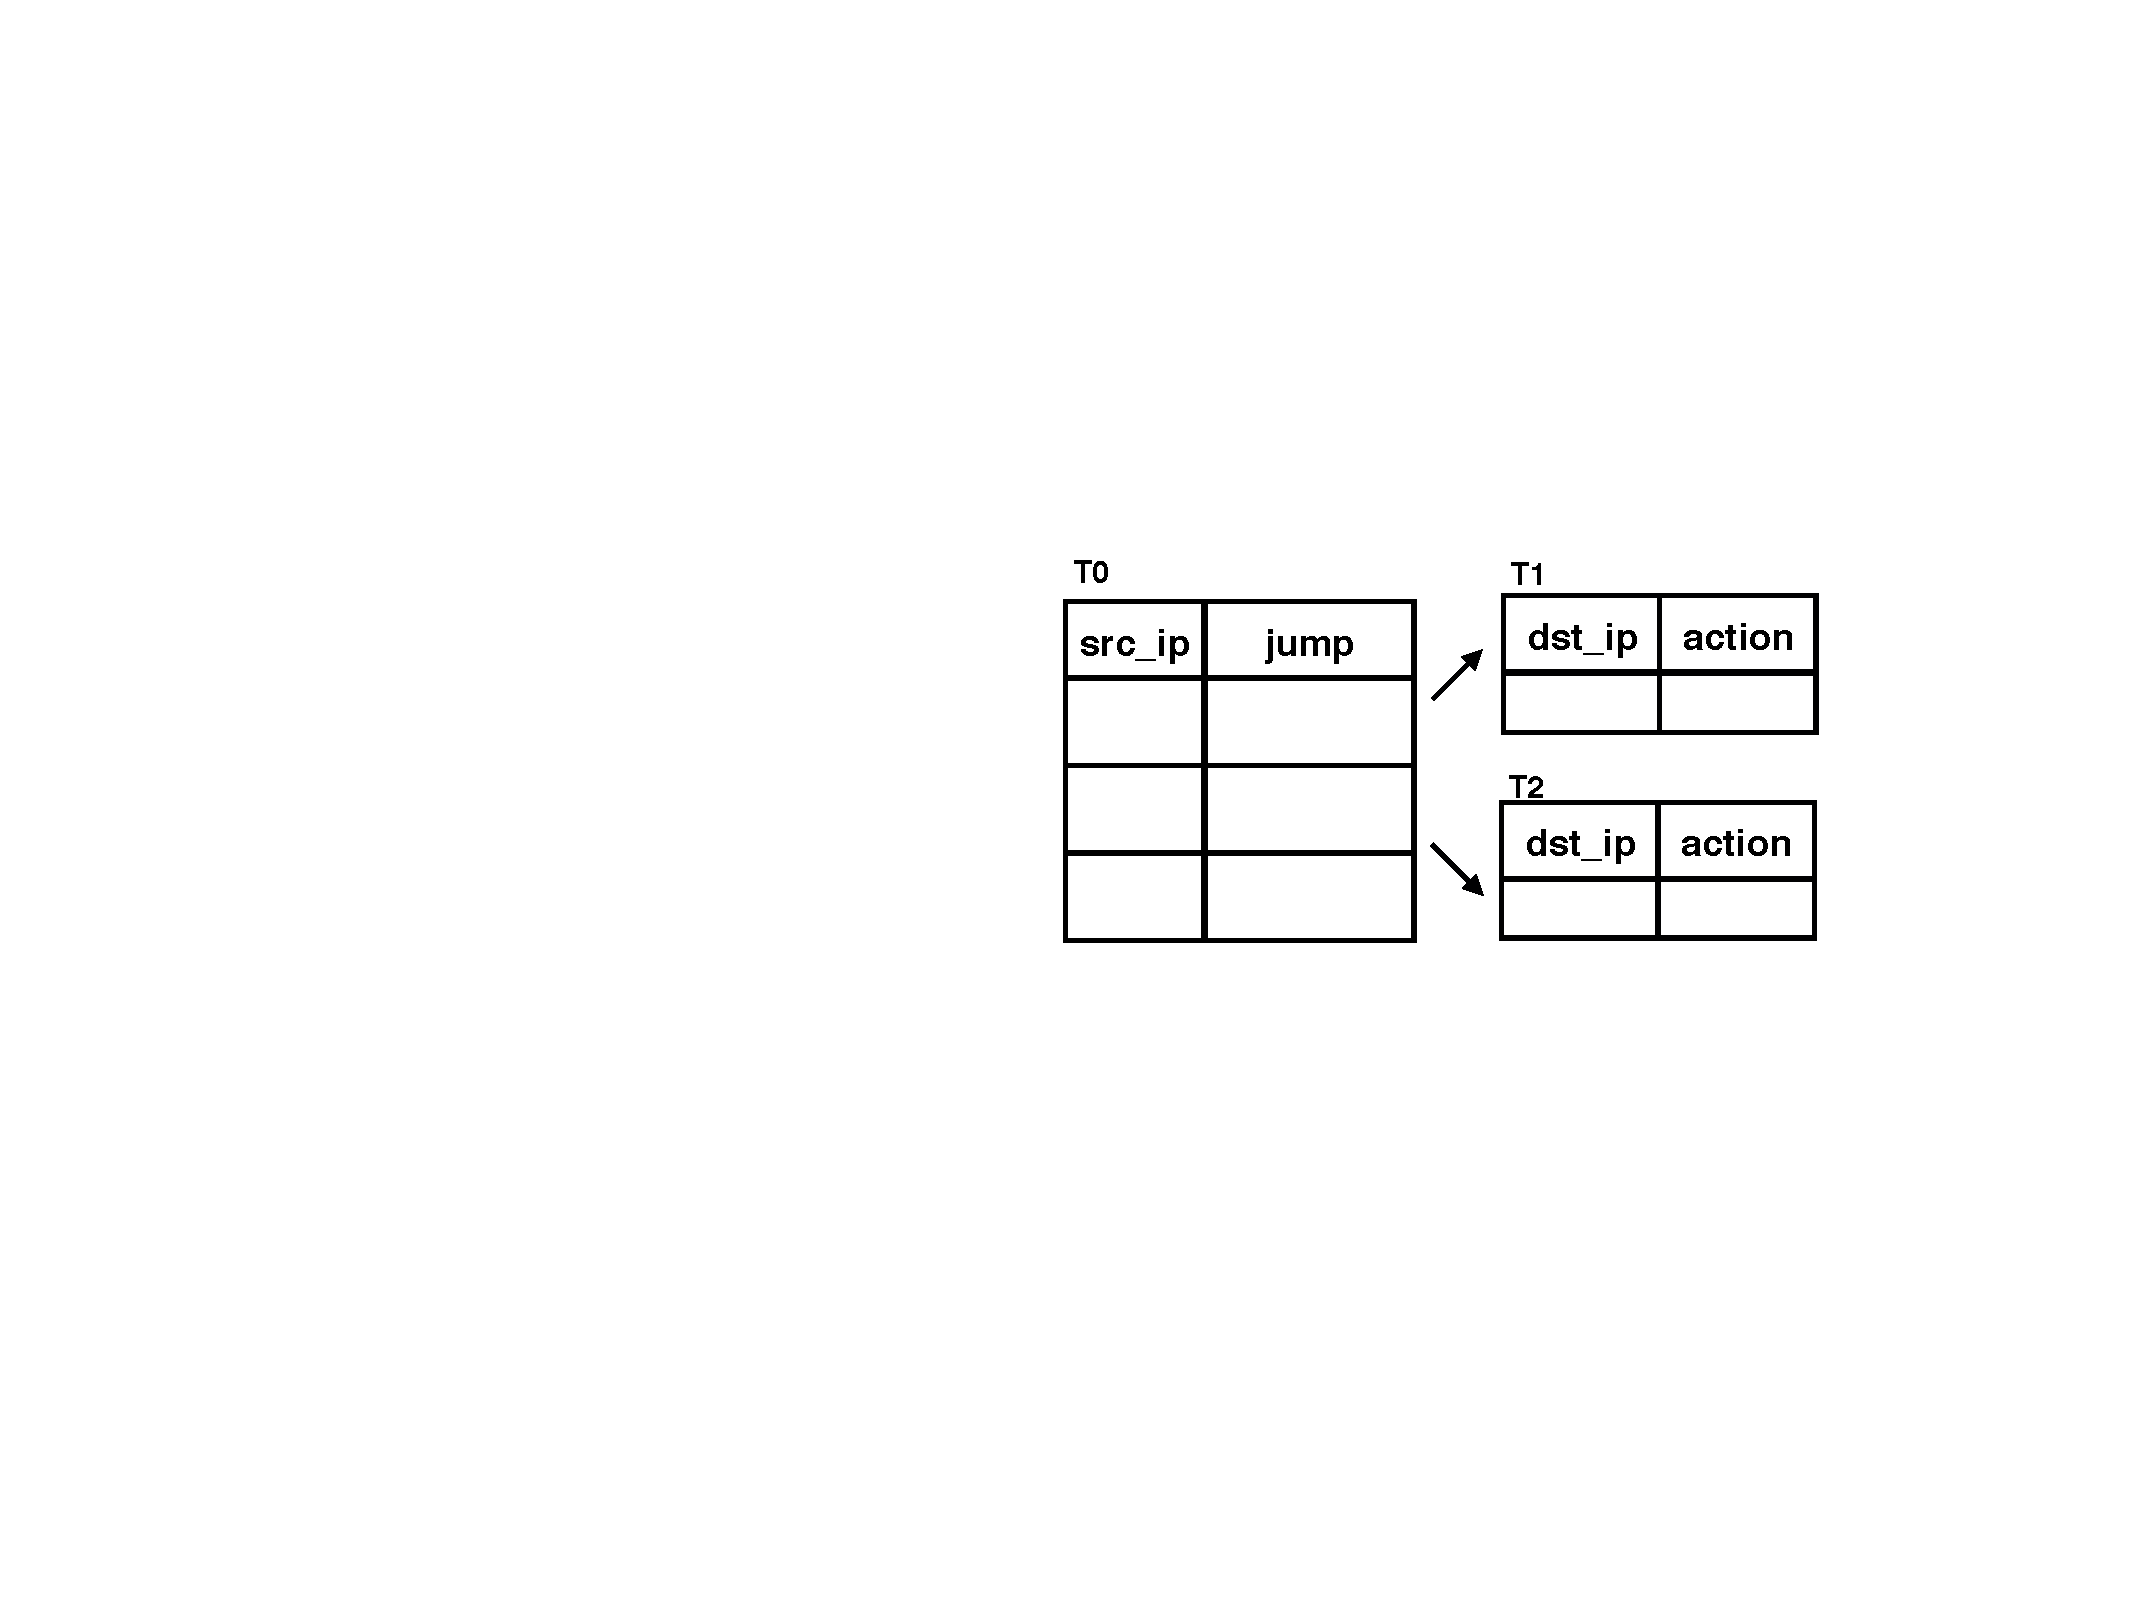
\includegraphics[width=3.25in]{figures/fig1-update.pdf}
%%    \vspace{-0.3in}
%    \caption{Example datapath.}
%    \label{fig:fig1-update}
%\end{figure}

% Solving the datapath programming capacity problem, however, is not trivial. Consider a high-level program \texttt{onPkt} shown in Sec.~\ref{sec:model-and-main-results}. The if statements in the program make the structure complex and the flexibility of table design makes the formalization of program hard. It is not desirable to make much restriction on programmers when they are writing high-level programs. Also, from the other side, consider a pipeline \texttt{swP} shown in Sec.~\ref{sec:model-and-main-results} Though the pipeline \texttt{swP} also defines a set tables, the layout might be different with the program \texttt{onPkt}, which including the pipeline structure and table matching fields. For example, the program \texttt{onPkt} requires a table matching both $dstAddr$ and $dstPort$ which does not exist in the pipeline \texttt{swP}. It is not obvious to see whether the program can be realized on the pipeline. 




%Fig.~\ref{fig:fig1-update}, which shows a simple datapath, named Example-DP, which consists of two-tables forming a pipeline. 
%Consider two simple high-level SDN programs [revise]. An interested reader can try to verify that the first program can be realized by Example-DP, but the second cannot. 
%{\small
%\begin{verbatim}
%// Program: L3-Route
%
%   onPacket(p):
%1.   s = p.srcIP
%2.   d = p.dstIP
%3.   if (s == "10.0.0.1"):
%4.     egress = myPolicyOne(d)
%5.   else
%6.     egress = myPolicyTwo(d)
%8.   return egress
%\end{verbatim}
%}
%
%{\small
%\begin{verbatim}
%// Program: L3-Route-Changed
%...
%4.   if (s == "10.0.0.1"):
%5.     egress = myPolicyOne(d)
%6.   else if (s == "10.0.0.2"):
%7.     egress = my PolicyThree(d)
%...
%\end{verbatim}
%}

%Consider a high-level program \texttt{onPkt} shown in Sec.~\ref{sec:model-and-main-results}. The if statements in the program make the structure complex and the flexibility of table design makes the formalization of program hard. It is not desirable to make much restriction on programmers when they are writing high-level programs. Also, from the other side, consider a pipeline \texttt{swP} shown in Sec.~\ref{sec:model-and-main-results} Though the pipeline \texttt{swP} also defines a set tables, the layout might be different with the program \texttt{onPkt}, which including the pipeline structure and table matching fields. For example, the program \texttt{onPkt} requires a table matching both $dstAddr$ and $dstPort$ which does not exist in the pipeline \texttt{swP}. It is not obvious to see whether the program can be realized on the pipeline. 



Solving the datapath capacity problem, however, is not trivial. 
Consider a simple datapath, named Simple-DP, shown in Fig.~\ref{fig:fig1-update}. It is among the simplest datapaths, consisting of three tables forming a pipeline, where the first table (\texttt{t1}) matches on source IP and may jump to one of the two following tables, which both match on destination IP.
\begin{figure}[h!]
    \centering
    \vspace{-0.1in}
    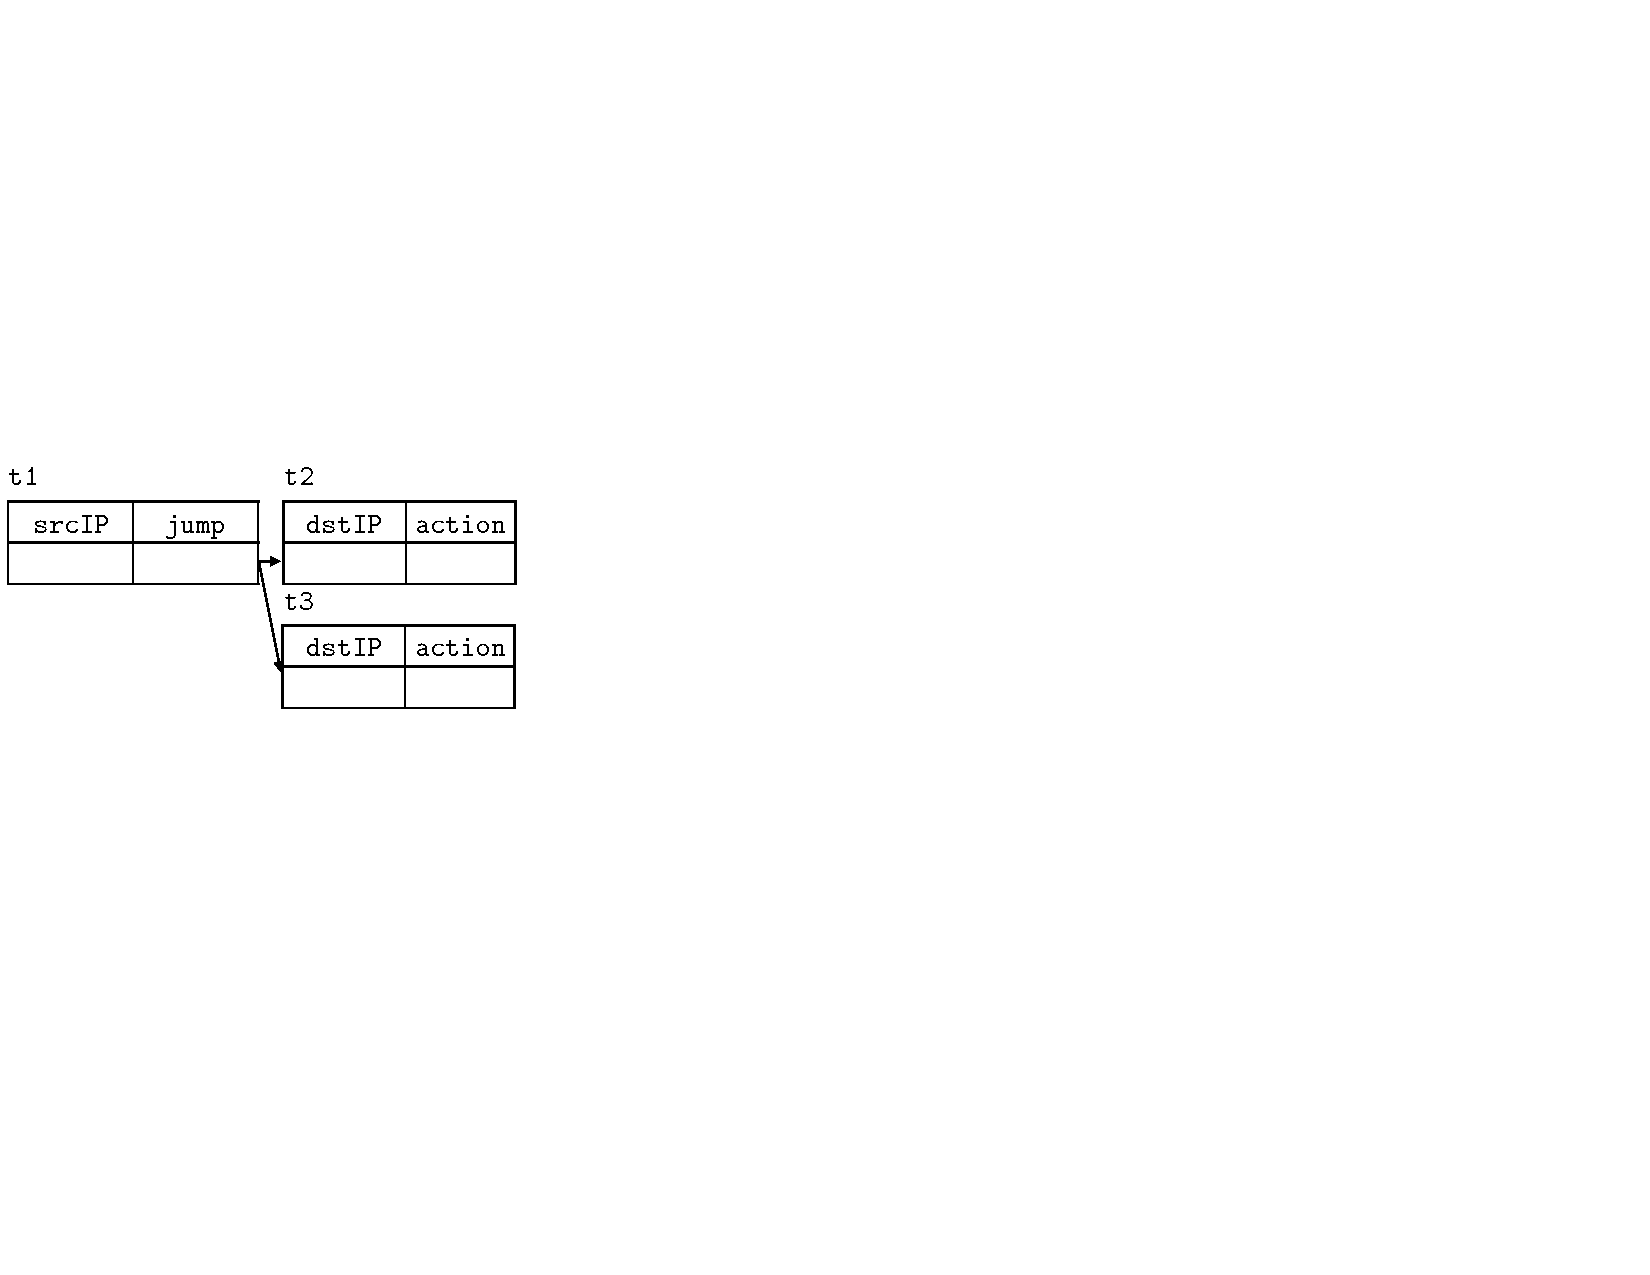
\includegraphics[scale = 0.7]{figures/figure1.pdf}
    \vspace{-0.1in}
    \caption{A simple example datapath: Simple-DP.}
    \vspace{-0.1in}
    \label{fig:fig1-update}
\end{figure}

Consider two simple high-level SDN programs below, both specified in the algorithmic, event-driven programming style to handle packet misses; see Sec. II for more details on the programming model. An interested reader can try to verify that the first program can be realized by Simple-DP, but the second cannot. 
{\small
\begin{verbatim}
//  Routing Function: secureL3Route
L0: secureL3Route(Addr srcIP, Addr dstIP):
L1:   if srcIP == 10.0.0.1:
L2:     return Forward(port=shortestPath(dstIP))
L3:   else:
L4:     return Drop();
\end{verbatim}
}

{\small
\begin{verbatim}
//  Program: twoHostL3Route
L0: def twoHostL3Route(Addr srcIP, Addr dstIP):
L1:   if srcIP == 10.0.0.1:
L2:     return Forward(port=shortestPath(dstIP)) 
L3:   elif srcIP == 10.0.0.2:
L4:     return Forward(port=securePath(dstIP))
L5:   else:
L6:     return Drop();
\end{verbatim}}

Although the preceding datapath and high-level programs are among the simplest, they may already appear to be non-trivial for a reader to analyze. General datapath and high-level programs can be much more complex as multiple services need to be implemented and hence they can pose severe challenges in analysis. The goal of this paper is to develop the first systematic methodology to solve the SDN datapath programming capacity problem. 

The contributions of this paper can be summarized as follows. First, we  propose a unifying characteristic functional space to unify and extract the essence of programs and pipelines, removing complexities such as program structures and pipeline layouts. Second, we define a comparator in this functional space, which can be used to check whether a high-level program can be realized on a given pipeline.

The rest of the paper is organized as follows. We define our model precisely in Sec.~\ref{sec:model-and-main-results}. The main results are given in Sec.~\ref{sec:main-results} and the proofs are shown in Sec.~\ref{sec:proofs}. Sec.~\ref{sec:evaluation} shows our evaluation results. Finally, related work is provided in Sec.~\ref{sec:related-work}.

\title{PC Model}

\date{\today}

\documentclass[12pt]{article}
\usepackage{sectsty}
\usepackage{graphicx}
\usepackage{etoolbox}
\usepackage{amsmath}
\usepackage{amssymb}
\usepackage{mathabx}

\sectionfont{\fontsize{12}{15}\selectfont}
\subsectionfont{\fontsize{12}{15}\selectfont}

\makeatletter
\patchcmd{\@verbatim}
  {\verbatim@font}
  {\verbatim@font\fontsize{8}{10}\selectfont}
  {}{}
\makeatother

\begin{document}
\maketitle

\section{Functions}
\begin{itemize}
  \item Routing function: $f$
  \item Set of $\forall$ routing functions: $\mathcal{F}$
  \item Packet match fields read by $f$: $\langle m_1, ..., m_n \rangle$
  \item Set of $\forall$ packet match fields read by $f$: $\mathcal{M}$
  \item Subset of $\mathcal{M}$: $M_i$
  \item Values of packet match fields $M_i$ in a call to $f$: $v_i(M_i)$
  \item Domain of valid packet match field values of M: $dom(M_i)$
  \item Set of $\forall$ routing actions: $\mathcal{R}$
\end{itemize}

\begin{equation} 
 f : dom(\mathcal{M}) \rightarrow \mathcal{R}
\end{equation}

\section{Pipelines}
\begin{itemize}
  \item Pipeline: $p$
  \item Set of $\forall$ pipelines: $\mathcal{P}$\
  \item $p$ is a singly rooted dag of tables $t_i$ \textit{s.t.} an edge $(t_i, t_j)$, indicates control flow may pass from $t_i$ to $t_j$.
  \item We assume the set of packet match fields $p$ reads is the same as the set $f$ reads, and carry terminology over (\textit{e.g.} $\mathcal{M}$, $M_i$, $dom(M_i)$).
  \item We denote `$f$ is embeddable into $p$' as: $f \rightrightharpoons p$.
\end{itemize}

\section{Tables}

\subsection{Table outputs}
\begin{itemize}
  \item A $t_i$'s outputs may be some combination of:
  \begin{itemize}
      \item Pipeline egress actions
      \item Writes to $t_i$'s output register, $r(t_i)$
      \item Transfer of control to a subsequent table $t_j$
  \end{itemize}
  \item Register $r(t_i)$ has size $|r(t_i)|$.
  \item If $t_i$ may output to a pipeline egress, we say $t_i$ is an egress table.
\end{itemize}


\subsection{Table inputs}
\begin{itemize}
  \item A $t_j$'s inputs $I(t_j)$ may be some combination of:
  \begin{itemize}
      \item Packet match fields read by $p$, $m_i \in \mathcal{M}$
      \item A $t_i$'s output register $r(t_i)$
  \end{itemize}
\end{itemize}

\subsection{Table rules}
\begin{itemize}
  \item The maximum number of rules a $t_i$ can contain is: $maxrules(t_i)$
\end{itemize}
\end{document}
\section{Main Results}
\label{sec:main-results}

%\yry{search realize and change to realize; introduce the realize symbol in main text.}
Given the function and pipeline models, we now present our main results, on whether a function $f$ can be realized by a pipeline $p$.

To simplify the reading of our results, we put only the definitions and main results in the main text. The proofs of the results are in the appendix. To make it easier to follow the symbols, we collect key symbols in Table I for reference.

\begin{table}
\centering
\begin{tabular}{| l | l |}
  \hline
  \textbf{Symbol} & \textbf{Definition}\\
  \hline
  \hline
  \multicolumn{2}{|l|}{\textbf{Routing function symbols}} \\
  \hline
  $f$ & Routing function\\
  $\mathcal{F}$ & Routing function space\\
  $m_i$ & Packet match field\\
  $\mathcal{M}$ & Set of $\forall\ m_i$\\
  $dom(M)$ & Domain of valid values of $M$\\
  $\mathcal{R}$ & Set of $\forall$ valid routing actions\\ 
  \hline
  \hline
  \multicolumn{2}{|l|}{\textbf{Pipeline symbols}} \\
  \hline
  $p$ & Pipeline\\
  $\mathcal{P}$ & Pipeline function space\\
  $t_i$ & Pipeline table\\
  $r(t_i)$ & $t_i$'s output register\\
  $bits(r(t_i))$ & $t_i$'s output register bit length\\
  $I(t_i)$ & $t_i$'s table inputs\\
  $maxrules(t_i)$ & Maximum $\#$ of rules $t_i$ can contain\\
  \hline
\end{tabular}
\vspace{2mm}
\label{tbl:sym-table}
\caption{Symbol table listing notation in our main results.}
\end{table}

\subsection{Overview}
%---\yry{we denote xxx when f can be realized by p}--
A main challenge in developing a systemic method to verify whether a routing function $f$ can be realized by a pipeline $p$, which we denote as $f \rightrightharpoons p$, is that routing functions and pipelines are represented differently and both types of representations can have substantial complexities and variations. Consider each routing function $f$ as a point in a functional space $\mathcal{F}$, and each pipeline $p$ as a point in functional space $\mathcal{P}$. 

Our main contribution is the introduction of a novel, unifying, normalization functional space $\mathcal{C}$ called the characteristic functions space. Each routing function $f$ is mapped by the mapping $\tau$ to a characteristic function $\tau(f) \in \mathcal{C}$, characterizing the computational load of $f$. Each pipeline $p$, on the other hand, is mapped to a set $\kappa(p) \subset \mathcal{C}$ of characteristic functions, representing the set of computational capabilities of the pipeline. 
Fig~\ref{fig:function-spaces} illustrates the mapping structure.

%The main structure of our main result is that we can then define a third, ordered space , the space of $\forall\ c$ and produce mappings from $\mathcal{F}$ and $\mathcal{P}$ to $\mathcal{C}$ and $2^\mathcal{C}$ which we denote $\tau$ and $\kappa$ respectively. These three spaces $\mathcal{F}$, $\mathcal{P}$ and $\mathcal{C}$ and the mappings between them in are shown in Fig~\ref{fig:function-spaces}.

\begin{figure}[tbh]
    \centering
    \vspace{-1mm}
    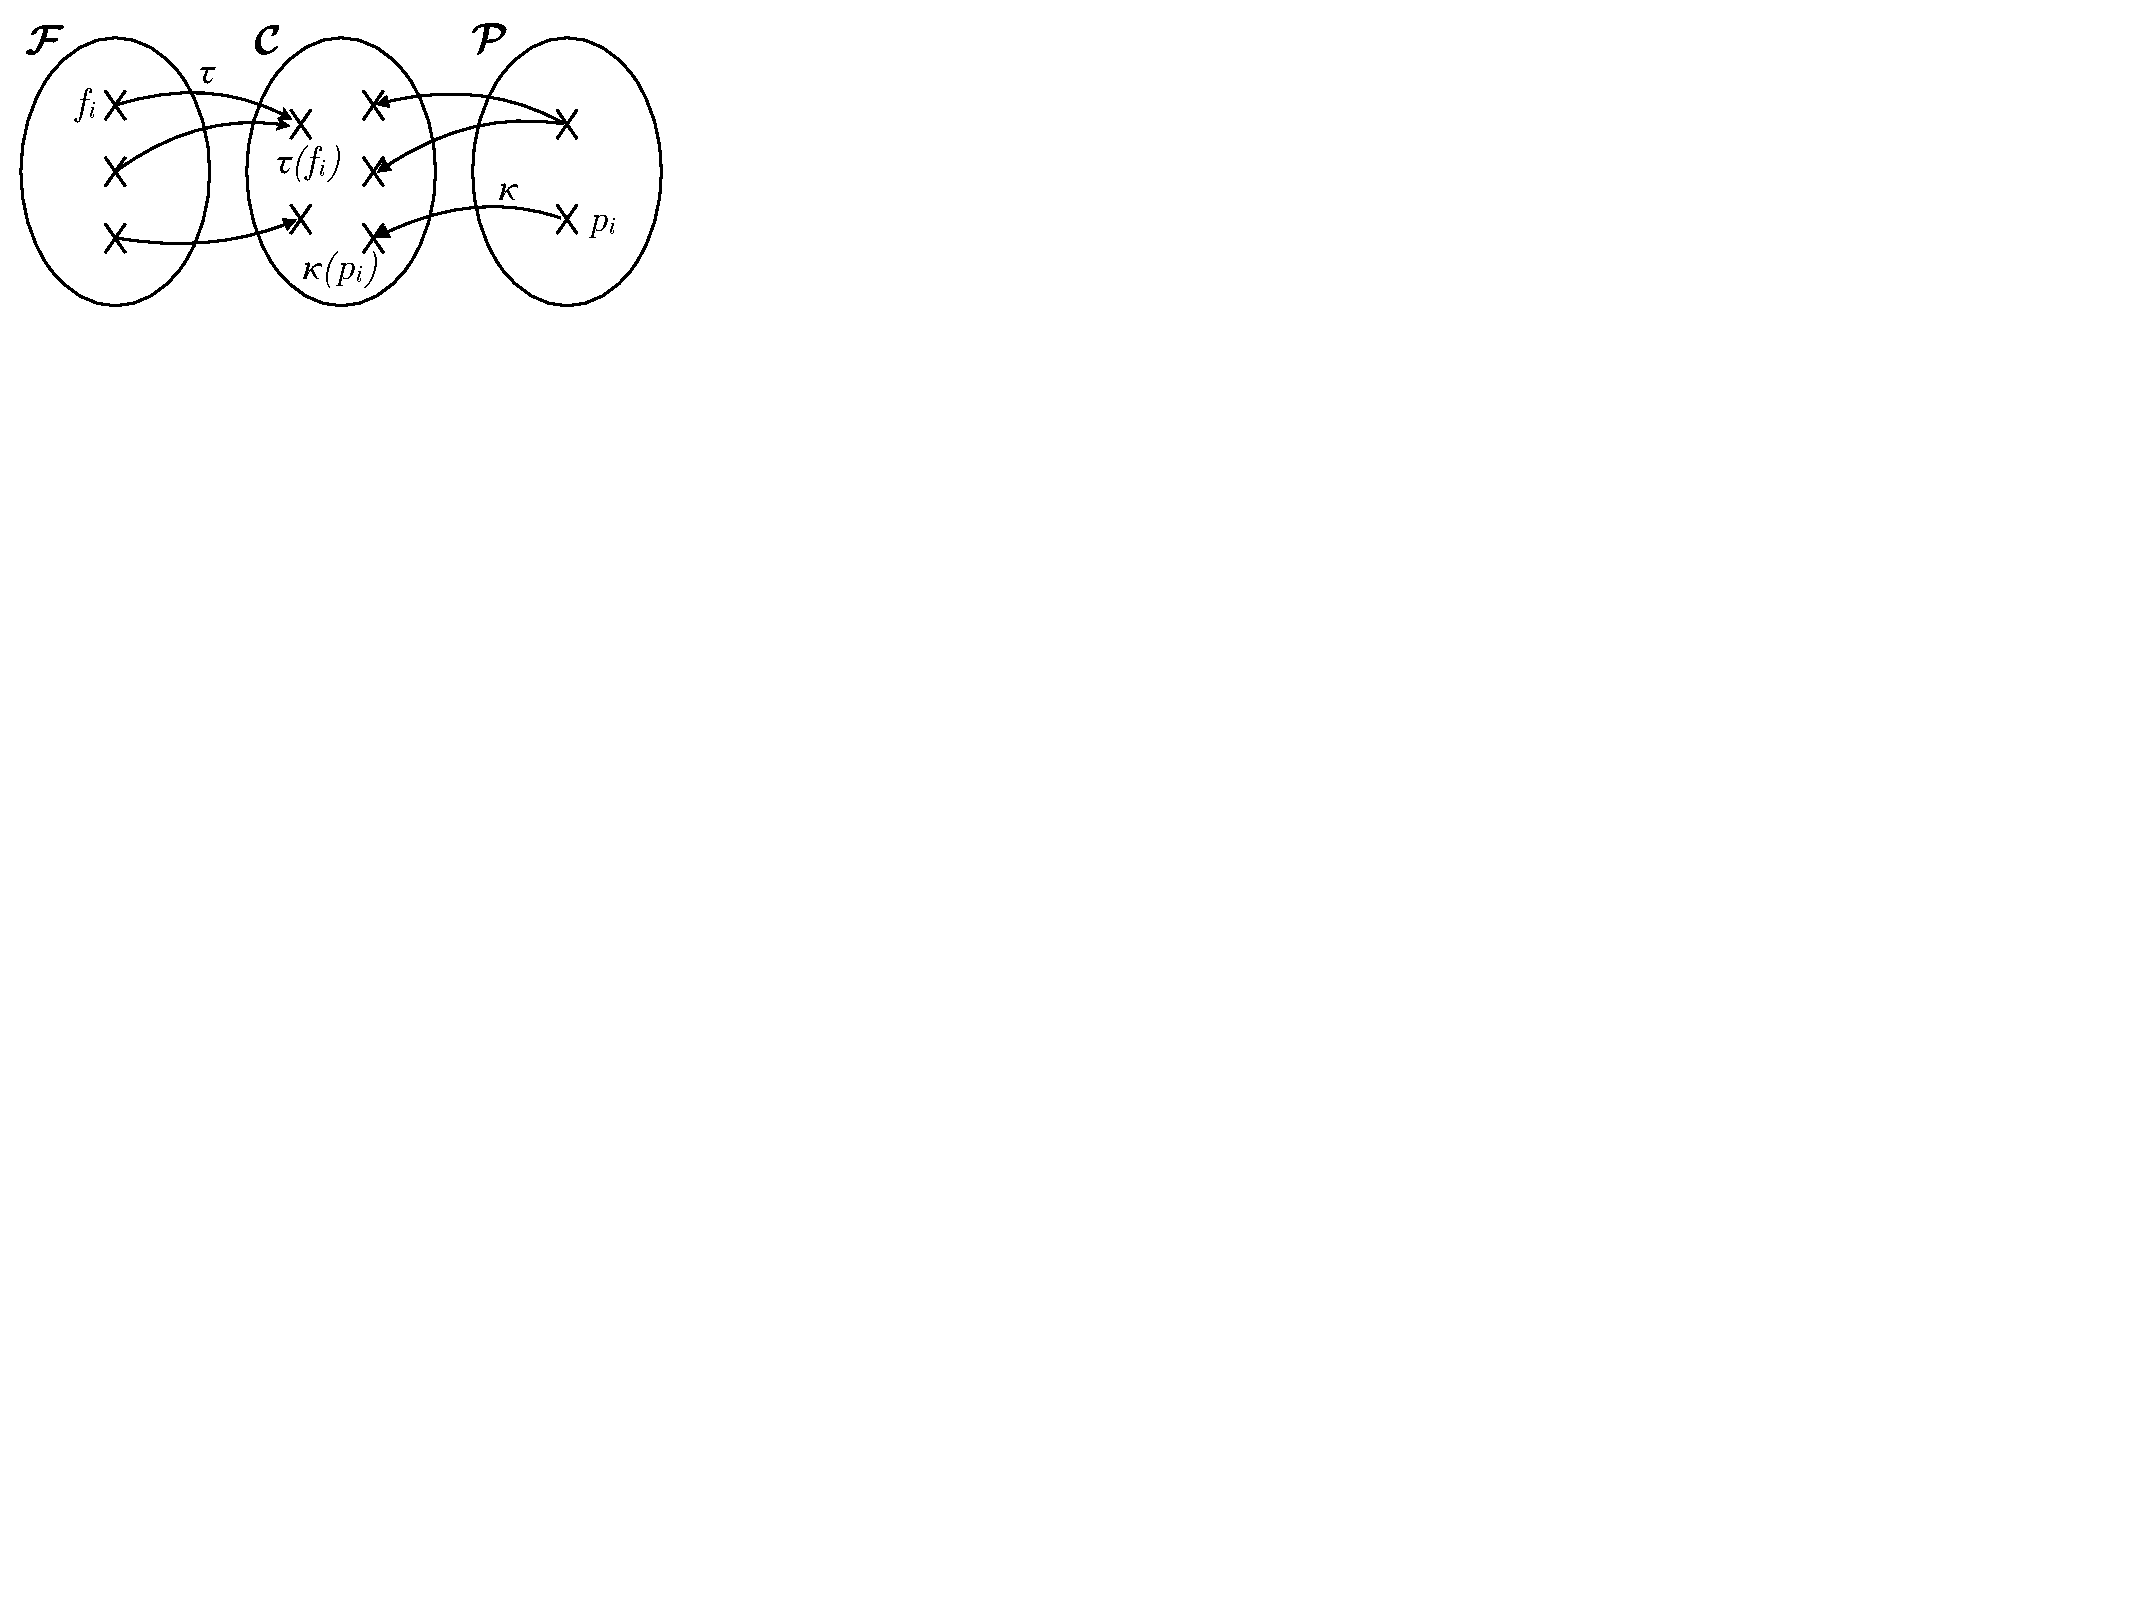
\includegraphics[clip, trim=0in 8.5in 9.8in 0in, width=2in]{figures/function-spaces.pdf}
    \vspace{-2mm}
    \caption{The spaces $\mathcal{F}$, $\mathcal{P}$ and $\mathcal{C}$ and the mappings between them.}
    \label{fig:function-spaces}
    \vspace{-2mm}
\end{figure}

Since $\tau(f)$ and $\kappa(p)$ are defined in the the same space $\mathcal{C}$, as a point and as a set of points respectively, one can compare $\tau(f)$ with each element in $\kappa(p)$, to see if the load can be "covered" by a capability, resulting in our basic capacity theorem: that if $\exists\ c \in \kappa(p) \geq \tau(f), f \rightrightharpoons p$.

%Finally, we define a set of operators which act on $\mathcal{C}$ that calculate the joint characteristic functions of composed functions and networks of pipelines from their constituent functions and pipelines' characteristic functions, extending our embedding theorem to multi-pipeline networks and multi-function programs.

\subsection{Characteristic Functions}
% To determine if an $f$ is embeddable into a $p$, we require a way of comparing $f$ and $p$. XX $f$ and $p$, however, have very different formats, making side by side comparison highly unintuitive. The key insight that makes such comparison possible is that we can ...

%is that both $f$ and $p$ represent computations. The main contribution of this paper is that we can find a common characterization for these computations, which we define using the notion of characterization functions.

% Our characterization function extracts the key properties of a computation (routing functions) or computational capacity (pipelines) in a form that permits comparison. Surprisingly, these properties are simply the domain $dom(M)$ and range $range(M)$ for every subset $M$ of the set of match fields. 

% \begin{definition}
% The {\em domain $dom(M)$} of a subset $M$ of match fields is the set of values ... can take.
% \end{definition}

% \begin{definition}
% The {\em range $range(M)$} of ... is the set of values of a subset $M$ of match fields that can be distinguished.
% \end{definition}

% Domain and range can take any positive integer or a special value, $\intercal$, treated as positive infinity, which denotes a field whose value can be ignored. 

We begin by defining a generic characteristic function $c$.
\begin{definition} A {\em characteristic function $c$} is a mapping from each subset $M$ of a packet's match fields to a vector consisting of two components: 
\begin{equation*}
c(M) \overset{\Delta}{=} <scope(M),\ ec(M)>.
\end{equation*}
\end{definition}

%\yry{fix} 
We refer to the two components of $c(M)$'s vector as $c(M)[scope]$ and $c(M)[ec]$ respectively.


%Suprisingly, these properties are simply the domain and a property we denote \textit{f-equivalence class number} of every subset of a computation's inputs $M \in 2^\mathcal{M}$. 

%We will offer intuition into the behavior of these properties when we define mappings from $\mathcal{F}$ and $\mathcal{P}$ to $\mathcal{C}$. For now it suffices to state that these properties' values can be positive integers or a special value, $\top$, which we interpret as positive infinity, and thus our characteristic function is simply the mapping:

%\begin{equation}
%c : 2^\mathcal{M} \rightarrow (\mathbb{N} + \{\top \})^2\\
%\end{equation}

%We use our mapping to define a partial order over $\mathcal{C}$ by equipping $\mathcal{C}$ with the comparator:

%, we define a comparator over $\mathcal{C}$. Our comparator equips $\mathcal{C}$ with a partial order. 
Given two characteristic functions, one can compare them. 

\begin{definition}We define {\em $c_i$ dominates $c_j$}, denoted as $c_i \geq c_j$ as follows:
\begin{equation*}
\begin{split}
c_i \geq c_j \overset{\Delta}{=}\ \forall\ n \in\ &\{scope, ec\},\\
&\forall\ M \in 2^\mathcal{M},\ c_i(M)[n] \geq c_j(M)[n].
\end{split}
\end{equation*}
\end{definition}

To verify our capacity theorem, we need to compare a set of characteristic functions with a single characteristic function.

%Below we need ..., we define a comparator $\trianglerighteq$ between a $C \in 2^\mathcal{C}$ and a $c \in \mathcal{C}$ from Definition~\ref{def:comparator}.

\begin{definition}
A set of characteristic functions $C_i$ {\em dominates} a characteristic function $c_j$, denoted as $C_i \trianglerighteq c_j$, if a $c_i \in C_i$ dominates $c_j$:

\begin{equation*}
C_i \trianglerighteq c_j \overset{\Delta}{=} \exists\ c_i \in C_i : c_i \geq c_j.
\end{equation*}
\end{definition}
 
\subsection{Characterization of a Routing Function} 
Given the concept of characteristic functions, we now derive the characteristic function, denoted as $\tau(f)$, of a routing function $f$. 

\begin{definition}
\label{def:set-comparator}
The {\em scope} of the characteristic function of a routing function for a subset of packet match fields $M$ is the size of the domain of valid values of $M$:
\begin{equation*}
\tau(f)(M)[scope] \overset{\Delta}{=} dom(M)
\end{equation*}
\end{definition}

$\tau(f)(M)[ec]$ is a property that we build from the concept of f-equivalence: 
%We define f-equivalence $\sim_f$ as a binary property between values of $M$ which denotes that these values cannot be distinguished by $f$. We formalize it as follows:
\begin{definition} We define {\em f-equivalence}, denoted as $\sim_f$, as a relationship between two values of $M$, which we write as $v_i(M)$ and $v_j(M)$, which denotes that these values cannot be distinguished by $f$:
\begin{equation*}
\begin{split}
&v_i(M) \sim_f v_j(M) \overset{\Delta}{=} \forall\ v_k(\mathcal{M} - M) \in dom(\mathcal{M} - M),\\
&\qquad f(v_i(M), v_k(\mathcal{M} - M)) = f(v_j(M), v_k(\mathcal{M} - M)). 
\end{split}
\end{equation*}
\end{definition}

%A characteristic function maps each $M$ to xxx. For a routing function, compute the mapping in x way.  ...the proceed to define our mapping, denoted $\tau_e$, from a routing $f \in \mathcal{F}$ to its characteristic function $c \in \mathcal{C}$. We start by defining the properties, domain and equivalence class number, that a $c$ maps $\forall\ M \in 2^M$ to in the context of an $f$.

%The domain of a f's $M$ $dom(M)$, as we defined in our model of $f$, is simply the set of values of $M$ permitted by $f$. 

%The f-equivalence class number of an $f$'s $M$ is rooted in our concept of f-equivalence, $\sim_f$. f-equivalance is a binary property of values of $M$, $v_i(M) \sim_f v_j(M)$, and intuitively means that $v_i(M)$ and $v_j(M)$ are not distinguished by $f$, or more formally: 

%\begin{equation}
%\begin{split}
%v_i(&M) \sim_f v_j(M) \triangleq f(v_i(M), v_k(\mathcal{M} - M)) = \\ 
%&f(v_j(M), v_k(\mathcal{M} - M))\ \forall\ v_k(\mathcal{M} - M) \in dom(%\mathcal{M} - M)
%\end{split}
%\end{equation}

Our definition of f-equivalence leads naturally to our definition of an f-equivalence class. 
\begin{definition} An {\em f-equivalence class}, denoted as $[v_i(M)]_f$, is the set of all values f-equivalent to a given $M$'s value $v_i(M)$:
\begin{equation*}
[v_i(M)]_f \overset{\Delta}{=} \{v_j(M) \in dom(M) : v_i(M) \sim_f v_j(M)\}.
\end{equation*}
\end{definition}

Counting equivalence classes gives us the concept of f-equivalence class number.
 
\begin{definition}
The {\em f-equivalence class number} of $M$, denoted as $|dom(M)/\sim_f|$, is the cardinality of $M$'s set of f-equivalence classes. 
\end{definition}

We now arrive at our definition of $\tau(f)(M)[ec]$.

\begin{definition} The {\em ec} of a routing function's characteristic function for an $M$ is the cardinality of $M$'s set of f-equivalence classes: 
\begin{equation*}
\tau(f)(M)[ec] \overset{\Delta}{=} |dom(M)/\sim_f|
\end{equation*}
\end{definition}
%Given these definitions, we define the characteristic function $\tau(f)$ of an $f \in \mathcal{F}$ as:

% to its characteristic function $c \in \mathcal{C}$.

\begin{definition} {\em The characteristic function $\tau(f)$ of a routing function} characterizes $f$'s computational load:
\begin{equation*}
\tau(f)(M) \overset{\Delta}{=} (dom(M),\ |dom(M)/\sim_f|).
\end{equation*}
\end{definition}


%of $M$ is therefore simply the cardinality of the set of its f-equivalence classes, $|dom(M)/\sim_f|$.

%Our mapping from $f \in \mathcal{F}$ to their characteristic functions $\tau_e$ proceeds straightforwardsly from our definitions of domain and f-equivalence class number:

%\begin{equation}
%\begin{split}
%&\tau_e : \mathcal{F} \rightarrow \mathcal{C}\\
%&f \mapsto c : c(M) =(dom(M),|dom(M)/\sim_f|)\ \forall\ M \in 2^M
%\end{split}                   
%\end{equation}

While $\tau(f)$ is powerful it is impractical because f-equivalence class number is costly to directly calculate. We therefore bound a $\tau(f)$ by defining the bounding characteristic function of a routing function $\tau_G(f)$ which is easily derivable from $f$'s DFG. This function characterizes an upper bound on $f$'s computation load: $\tau_G(f)$ dominates $\tau(f)$.

We find $\tau_G(f)[scope]$ as before. Instead of calculating $\tau_G(f)[ec]$, however, we determine an upper bound for with the value of specific vertex cut in $G_f$, $f$'s DFG. We now construct this cut.

%Before we transform a routing function into a DFG we apply two key transformations. First, we enforce single state assignment, by breaking up and renaming multiply-assigned variables. Second, we replace if statements with guard variables, transforming control dependencies into data dependencies. For example, \texttt{L3} and \texttt{L4} of \texttt{onPkt} would be transformed from:
%\begin{verbatim}
%L3: if (verify(srcPort, srcIP)):
%L4:   dstCond = condTbl[dstIP, dstPort]
%\end{verbatim}

%to:
%\begin{verbatim}
%L3: g0 = verify(srcPort, srcIP)):
%L4: if g0: dstCond = condTbl[dstIP, dstPort]
%\end{verbatim}

%Given these transformations, we now define the concept of a DFG.

%\begin{definition}
%A DFG $G_f = (V_f, E_f)$ of a $f$ is a vertex weighted dag corresponding to a function such that: $V_f$ is the set of variables in a SSA $f$, the weights of a variable in $V_f$ is its domain size, and $E_f$ is a set of directed edges such that there is a directed edge between two variables if the source variable appears in the target variable's assignment.
%\end{definition}

%We now define a particular type of min-cut in a function's DFG.

%Specifically, we calculate $\tau_G(f)[ec]$ using a vertex min-cut we define below:
\begin{definition} Let $V_f(M)$ be the vertices of $m_i \in M$ in $G_f$, and $D_f(M)$ be the vertices in $G_f$ descended from $V_f(M)$. 
\vspace{2mm}

The {\em vertex-min-cut of $M$}, $G_f.vertexMinCut(M)$, is the product of the weights of the vertices in the minimum weight vertex cut severing $V_f(M)$ from $D_f(\mathcal{M} -M)$.
\end{definition}

%We have arrived at our definition of $\tau(f)[ec]$.

%\begin{definition} $\tau(f)(M)[ec] \overset{\Delta}{=} G_f.vertexMinCut(M)$ is the minimum weight set of vertices severing $V_f(M)$ from $D_f(M)$, and is a bound on $\tau_e(f)(M)[ec]$
%\end{definition}

Given this cut, we define $\tau_G(f)$ follows:

%Let $V_f(M)$ be the set of vertices in $G_f$ that represent $m_i \in M$ and $D_f(M)$ be the set of vertices in $G_f$ descended from $V_f(M)$. Then the range of an $f$'s characteristic function is $G_f.vertexMinCut(V_f(M),\ D_f(M))$.

%Given this concept, $\tau$, our second mapping from a routing function to its characteristic function is:

\begin{definition} {\em The characteristic function $\tau_G(f)$ of a routing function} characterizes an upper bound on $f$'s computational load; $\tau_G(f)$ dominates $\tau(f)$:
\begin{equation*}
\tau_G(f)(M) \overset{\Delta}{=} (dom(M),\ G_f.vertexMinCut(M)).
\end{equation*}
\end{definition}

\para{Example:} We illustrate these concepts with our example routing function \texttt{onPkt}.

Consider \texttt{onPkt}'s match fields \texttt{srcIP} and \texttt{srcPort}. Each are only read once: on \texttt{L3}, by the boolean function \texttt{isVerified}. Thus, while \texttt{srcIP} and \texttt{srcPort} may have many f-equivalence classes individually, (\texttt{srcIP}, \texttt{srcPort}) only has two: values that \texttt{isVerified} evaluates to $0$, and values it evaluates as $1$.

Suppose \texttt{onPkt} is a routing function for a small commercial network fronted by a NAT with $50$ hosts each running a limited set of applications that only use $200$ standard ports. Given this, $dom(\texttt{srcIP}, \texttt{srcPort}) = 10000$, and thus $\tau(\texttt{onPkt})(\texttt{srcIP}, \texttt{srcPort}) = (10000, 2)$. 

While the equivalence class number of (\texttt{srcIP}, \texttt{srcPort}) was straightforwards, the equivalence class number of most other subsets of \texttt{onPkt}'s inputs is not so obvious. We therefore bound $\tau(\texttt{onPkt})$ with $\tau_G(\texttt{onPkt})$, which we calculate using \texttt{onPkt}'s DFG $G_{\texttt{onPkt}}$, shown in Fig.~\ref{fig:onpkt-dfg}.

%While finding the equivalence class number of (\texttt{srcIP}, \texttt{srcPort}) is straightforwards, the number of equivalence classes of other subsets of \texttt{onPkt}'s inputs such as (\texttt{srcIP}, \texttt{srcPort}, \texttt{dstIP}) is less obvious, making it difficult to calculate $c_{e,\texttt{onPkt}}$. Fortunately, we can calculate $c_{\texttt{onPkt}}$ more simply by generating \texttt{onPkt}'s DFG $G_{\texttt{onPkt}}$, shown in Fig.~\ref{fig:onpkt-dfg}.

\begin{figure}[tbh]
    \centering
    \vspace{-1mm}
    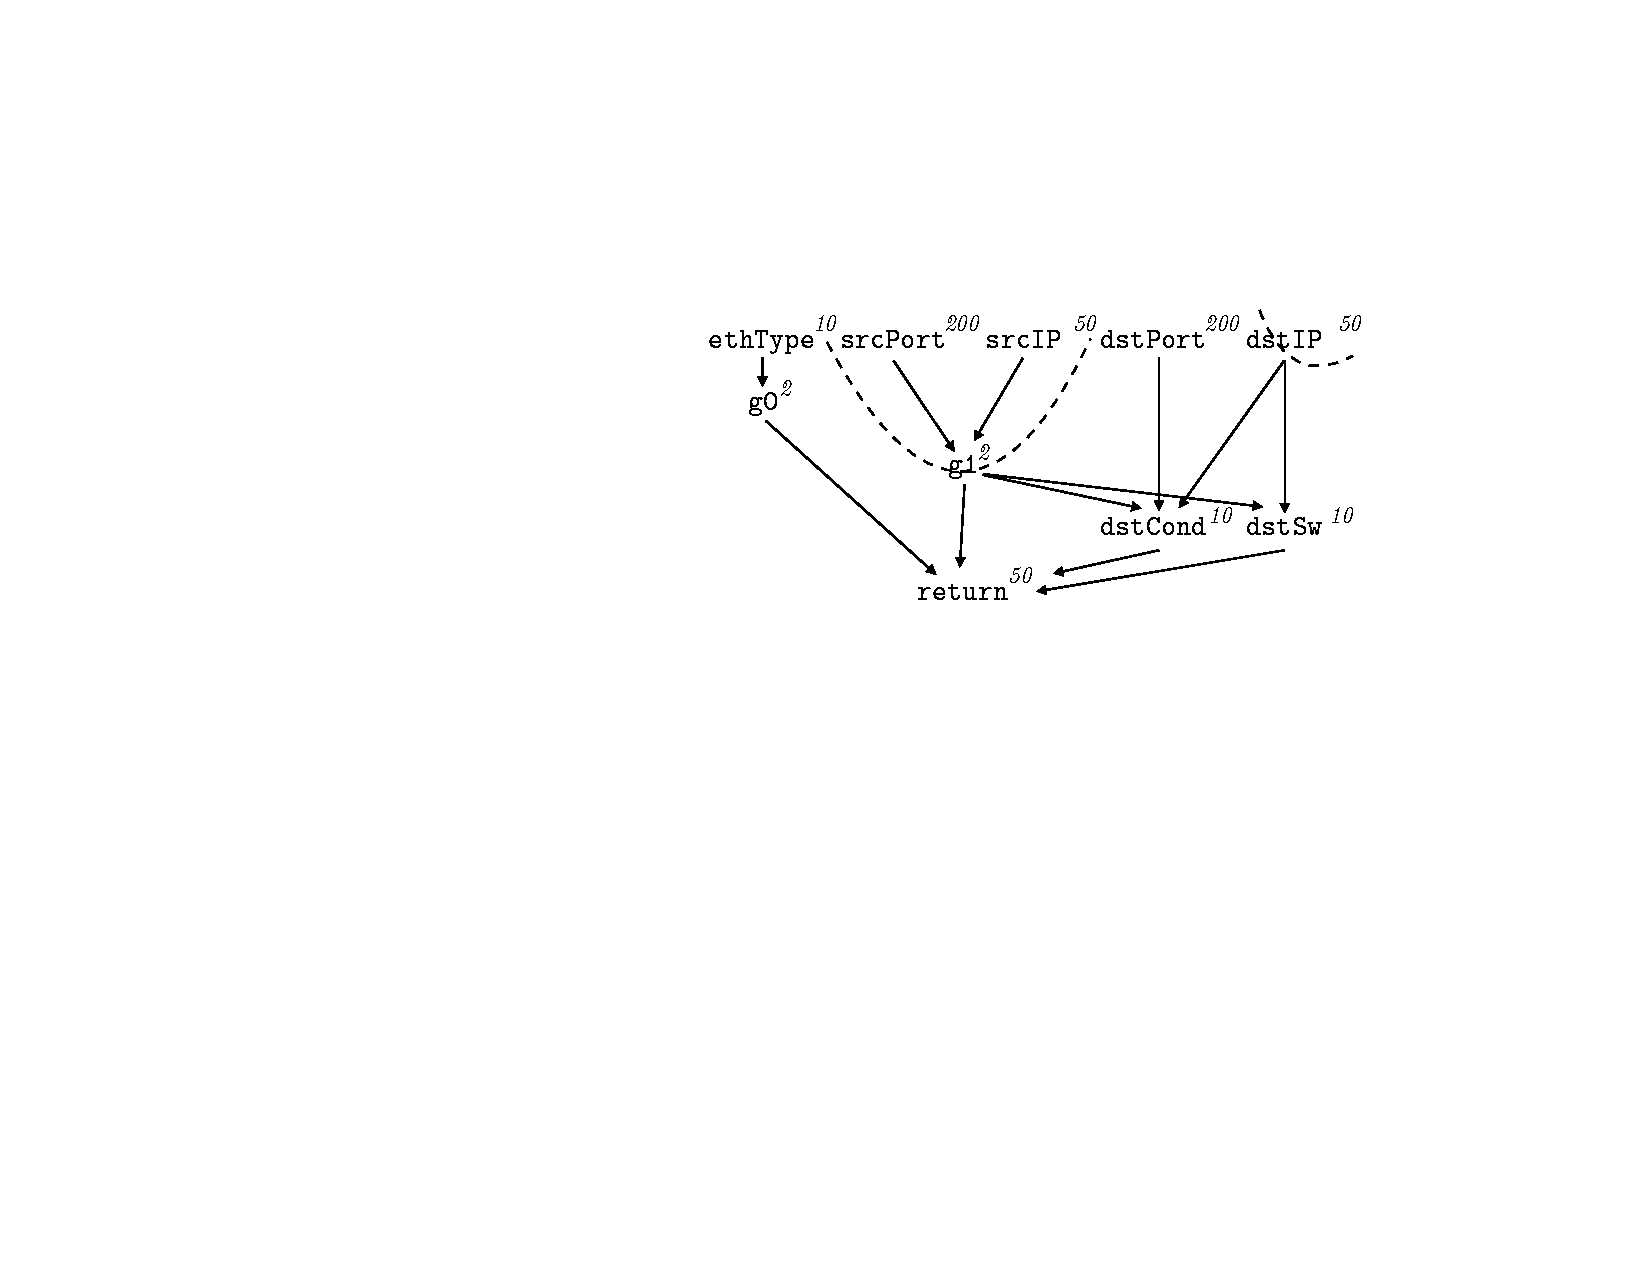
\includegraphics[scale = 0.6]{figures/figure5.pdf}
    \vspace{-2mm}
    \caption{The routing function \texttt{onPkt}'s DFG $G_{\texttt{onPkt}}$ and the cut $(\texttt{srcIP}, \texttt{srcPort}, \texttt{dstPort})$.}
    \label{fig:onpkt-dfg}
    \vspace{-2mm}
\end{figure}

%In $G_{\texttt{onPkt}}$, vertices such as \texttt{dstSw} correspond to \texttt{onPkt}'s variables, edges such as (\texttt{dstIP}, \texttt{dstSw}) imply that the source vertex \texttt{dstIP} is used in the target vertex \texttt{dstSw}'s assignment, and vertex weights such as $w(\texttt{srcIP}) = 50$ indicate their vertices' domain.

To bound, for example, the equivalence class number of \texttt{onPkt}'s inputs (\texttt{srcIP}, \texttt{srcPort}, \texttt{dstIP}) we take the vertex-min-cut in $G_\texttt{onPkt}$ between their vertices and every vertex descended from \texttt{onPkt}'s other inputs: (\texttt{ethType}, \texttt{dstPort},\texttt{g0}, \texttt{dstCond}, \texttt{return}). This vertex-min-cut is indicated in Fig.~\ref{fig:onpkt-dfg} by a dotted line.

%In $G_{\texttt{onPkt}}$, $G_{\texttt{onPkt}}.vertexMinCut(($\texttt{srcIP}, \texttt{srcPort}, \texttt{dstIP}$))$ is the product of vertex min cut weights between (\texttt{srcIP}, \texttt{srcPort}, \texttt{dstIP}) and the set of vertices descended from the remainder of \texttt{onPkt}'s inputs (\texttt{ethType}, \texttt{dstPort}): (\texttt{ethType}, \texttt{dstPort}, \texttt{g0}, \texttt{dstCond}, \texttt{return}), indicated by the dotted line in Fig.~\ref{fig:onpkt-dfg}. 

The vertices in this cut, (\texttt{g1}, \texttt{dstIP}) have weight $50$ and $2$, and thus $\tau_G(\texttt{srcIP}, \texttt{srcPort}, \texttt{dstIP}) = (50000,\ 100)$.


%The vertices in (\texttt{srcIP}, \texttt{srcPort}, \texttt{dstIP})'s vertex-min-cut are: (\texttt{g1}, \texttt{dstIP}) which have weight $50$ and $2$ respectively, and thus we find $100$ as an bound on this subset's number of equivalence classes. This implies that $c_\texttt{onPkt}(\texttt{srcIP}, \texttt{srcPort}, \texttt{dstIP}) = (50000,\ 100)$.

%he set of verticies in $G_f$ that represent $m_i \in M$ be $V_f(M)$

%Unfortunately, while $\tau_e$ is powerful, f-equivalence class number is costly to directly calculate and difficult to work with. Thus, in practice, we approximate $\tau_e$ with a second mapping from $\mathcal{F}$ to $\mathcal{C}$, $\tau$.

%The key insight underlying $\tau$ is that we can approximate f-equivalence class number using an $f$'s DFG, $G_f = (V_f, E_f)$. An $f$'s DFG is... \cleet{TODO: Define DFG}

%Given our description of an $f$'s DFG, our approximation for f-equivalence class number quickly follows. If the set of vertices in $V_f$ that represent a given $M$ is $V_f(M)$ and the set of vertices in $V_f$ descended from $V_f(M)$ is $D_f(M)$, we can approximate $|dom(M)/\sim_f|$ as the vertex min-cut separating $D_f(M)$ from $V_f(M)$ (which may include vertices in $V_f(M)$), which we denote as: $G_f.vertexMinCut(V_f(M),\ D_f(M))$. Substituting this approximation for $M$'s equivalence class number into $\tau_e$ yields $\tau$:

%\begin{equation}
%\begin{split}
%&\tau : \mathcal{F} \rightarrow \mathcal{C}\\
%&f \mapsto c : c(M) = (dom(M),\\
%&\qquad G_f.vertexMinCut(V_f(M),\ D_f(M))\ \forall\ M \in 2^M
%\end{split}                   
%\end{equation}

%\para{Example:} \cleet{TODO: Add example}

%....The first component of We begin by noting that routing functions can be very complex. Such functions may employ arbitrary computation to generate arbitrary mappings between the space of all packet header values and the space of all routing actions. Such spaces, furthermore, may be large. An IPv6 header alone, for example, contains 40 bytes of information, and typical routing functions increasingly read multiple headers spanning multiple layers of the internet stack. Our main result collapses this complexity, distilling routing functions down to their essential information transmission requirements.


%We begin by introducing the notion of f-equivalence, which we will use to parameterize $f$ transmission requirements.
%\vspace{1mm}

%\noindent \textsc{Definition 1 - f-equivalence:} An $S \in 2^M$'s values $u$ and $v$ are f-equivalent iff $f(S = u, M-S) = f(S = v, M-S)\ \forall$ values of $ M-S$.
%\vspace{1mm}

%Our definition of f-equivalence leads naturally to the definition of a f-equivalence class:
%\vspace{1mm}

%\noindent \textsc{Definition 2 - f-equivalence classes:} A set of mutually f-equivalence values of an $S$.
%\vspace{1mm}

%Before continuing, we provide the reader with some intuition into how f-equivalence classes behave. Consider the $f$ \texttt{onPkt}, below:

%\begin{verbatim}
%def onPkt(Addr dstIP, Port dstPort):
%  if dstPort <= 1024:
%    egress = stdHostTbl[dstIP]
%  elif dstPort == 1025:
%    egress = usrHostTbl[dstIP]
%  else:
%    return Drop();
%  return Forward(egress);
%\end{verbatim}

%The domain of \texttt{onPkt}'s input \texttt{dstPort} is $2^{16}$, since the TCP protocol allows TCP sockets to take any port number between $0$ and $65535$. However, \texttt{onPkt} only depends very particularly on where \texttt{dstPort}'s value falls within this domain, specifically on whether \texttt{dstPort} is $\leq 1024$, $1025$, or $> 1025$. Regardless of the value of \texttt{dstIP}, \texttt{onPkt} will always output the same result for any values of \texttt{dstPort} in the same set. Thus, we say that values within these sets are equivalent, and that the sets themselves comprise \texttt{onPkt}'s equivalence classes.

%We use our definition of f-equivalence classes to define the central abstraction of our theorem: the header set equivalence class function $h$, which associates every $S \in 2^M$ with a number of f-equivalence classes.
%\vspace{1mm}

%\yry{Move to early}
%\noindent \textsc{Definition 3 - Header f-equivalence class function:} A mapping $h$ from $\forall\ S \in 2^M$ to a number of f-equivalence classes, $2^M \rightarrow \mathbb{N}$.
%\vspace{1mm}

%\noindent \textsc{Definition 4 - Header f-equivalence class function space:} The space of $\forall\ h$, $H$.
%\vspace{1mm}

%The space $H$ is a powerful space to consider because we can define a mapping from $\forall\ f \in F$ to exactly one $h \in H$, $\tau$, which we illustrate in Fig.~\ref{fig:function-spaces}. and define below:
%\vspace{1mm}


%\noindent \textsc{Definition 5 - Function header f-equivalence class map, $\tau$:} $\tau$ is a mapping $f \rightarrow h$, \textit{s.t.} $h(S)$ is $S$'s number of f-equivalence classes $\in f$.
%\vspace{1mm}

\subsection{Characterization of a Pipeline}
We now define $\kappa(p)$, the set of characteristic functions of a pipeline $p$. We start by defining a path $\rho$ through a pipeline $p$.

%\noindent{\em Overview}:??

\begin{definition}
A path, $\rho$, in a $p$ is a path through $p$'s dag $\langle t_1, ..., t_n \rangle$ such that $t_1$ is a root table and $t_n$ an egress table in the $p$.
\end{definition}

As an example, \exampledp\ contains two paths: $\langle \texttt{t1}, \texttt{t2}, \texttt{t3}, \texttt{t4}, \texttt{t5} \rangle$, and $\langle \texttt{t1}, \texttt{t6} \rangle$, which we denote as $\rho_{L2}$ and $\rho_{L3}$ respectively. 

We define, $\forall\ \rho \in p,\ \kappa_\rho(p)$ as the characteristic function of the a path through a pipeline. 

\begin{definition} {\em The characteristic function set $\kappa(p)$} of a $p$ is the union of $\forall\ \rho \in p$'s characteristic functions:
\begin{equation*}
\kappa(p)(M) \overset{\Delta}{=} \{c \in \mathcal{C} : c = \kappa_\rho(\rho)\ \forall\ \rho \in p\}.
\end{equation*}
\end{definition}

We now construct the characteristic function of a path $\rho$ by introducing the following definitions:

%Given these definitions, we arrive at $\kappa_\rho(\rho)$, the characteristic function of a $\rho$.

%Each $\rho$ has a characteristic function where $dom(M)$ is the maximum number of values of $M$ that $\rho$ can read and $range(M)$ is the maximum number of equivalence classes of $M$ $\rho$ can distinguish. We determine the values of $dom(M)$ and $range(M)$ by introducing the following definitions:

%First, we define the input closure $\bar{M}_\rho(t_i)$ of a $t_i$ in $\rho$ as:

\begin{definition} The {\em input closure $\bar{M}_\rho(t_i)$} of a table $t_i \in \rho$ is the set of inputs that $t_i$ can obtain information about:
\begin{equation*}
\begin{split}
\bar{M}_\rho(t_i) \overset{\Delta}{=} \{m_i \in \mathcal{M} :\ &m_i \in I(t_i)\ \vee\\ &m_i \in \bar{M}_\rho(t_j)\ s.t.\ r(t_j) \in I(t_i)\}.
\end{split}
\end{equation*}
\end{definition}

%Next, we define the closure set, $\bar{\bar{M}}_\rho(M)$ of a $\rho$ as:
\begin{definition} The {\em closure set, $\bar{\bar{M}}_\rho(M)$} of a $\rho$'s $M$ is the set of $t_i \in \rho$ with input closure $M$.
\begin{equation*}
\bar{\bar{M}}_\rho(M) \overset{\Delta}{=} \{t_i \in \rho : \bar{M}_\rho(t_i) = M\}. 
\end{equation*}
\end{definition}

Using these definitions, we define the characteristic function of a $\rho$ as:
\begin{definition} {\em The characteristic function $\kappa_\rho(\rho)$ of a $\rho$} characterizes the computational capacity of a $\rho$. 

$\kappa_\rho(\rho)[scope]$ is the maximum number of values of $M$ that $\rho$ can read and $\kappa_\rho(\rho)[ec]$ is the maximum number of equivalence classes of $M$ that $\rho$ can distinguish.

\begin{equation*}
\begin{split}
&\kappa_\rho(\rho)(M) \overset{\Delta}{=}\\
&\begin{cases}
\bar{\bar{M}}_\rho(M) \neq \emptyset \quad \quad (min[maxrules(t_i) : t_i \in \bar{\bar{M}}_\rho(M)],\\
\quad \quad \quad \quad \quad \quad \quad \quad  min[2^{bits(r(t_i))} : t_i \in \bar{\bar{M}}_\rho(M)])\\
\bar{\bar{M}}_\rho(M) = \emptyset \wedge \exists\ m_i \in M :\\
m_i \notin \bigcup_{t_i \in \rho} \bar{M}(t_i, \rho)\  \quad \quad \quad \quad \quad (1, 1)\\
otherwise, \quad \quad \quad \quad \quad \quad \quad \ \ \ \ \, \, \,  (\intercal, \intercal).
\end{cases}
\end{split}
\end{equation*}
\end{definition}

\para{Example:} As before, we provide intuition into the characteristic functions of pipelines using our example pipeline \exampledp.

Recall from our model that \exampledp{} contains two $\rho$: $\rho_{\texttt{L2}}$ and $\rho_{\texttt{L3}}$. Consider the table \texttt{t4}, only contained by $\rho_{\texttt{L3}}$. The input closure $\bar{M}_{\rho_{\texttt{L3}}}(\texttt{t4})$ is (\texttt{srcIP}, \texttt{srcPort}, \texttt{dstIP}) since \texttt{t4} reads \texttt{dstIP} and \texttt{r(t2)}, and \texttt{t2} in turn reads \texttt{srcIP} and \texttt{srcPort}. The closure set, $\bar{\bar{M}}_{\rho_\texttt{L3}}(\texttt{srcIP}, \texttt{srcPort}, \texttt{dstIP})$, of \texttt{t4}'s inputs in $\rho_{\texttt{L3}}$ is $\{\texttt{t4}\}$: \texttt{t4}'s input closure is unique.

Thus, $\kappa_{\rho_{\texttt{L3}}}(\bar{M}_{\rho_{\texttt{L3}}})$ $=$ $\kappa_{\rho_{\texttt{L3}}}(\texttt{srcIP}, \texttt{srcPort}, \texttt{dstIP})$ $=$ $(maxRules(\texttt{t4}),$ $2^{bits(r(\texttt{t4}))})$. In the case that \texttt{t4} has $2^{20}$ rules and a $16$ bit output register, $\kappa_{\rho_{\texttt{L3}}}(\bar{M}_{\rho_{\texttt{L3}}}) = (2^{20}, 2^{16})$.

Further, consider the subset of \exampledp's match fields $(\texttt{srcMac},\ \texttt{dstMac})$. $\rho_{\texttt{L3}}$ does not contain the inputs \texttt{srcMac} or \texttt{dstMac} and thus it can only realize functions that contain them in the unlikely event that all are constants.  Constants have domain $1$ and $1$ equivalence class. Thus the value of $\kappa_{\rho_{\texttt{L3}}}$ for any set of outputs containing \texttt{srcMac} is $(1, 1)$.

Finally, consider the subset of \exampledp's match fields $(\texttt{srcIP},\ \texttt{srcPort})$. \texttt{srcIP} and \texttt{srcPort} are both read by $\rho_{\texttt{L3}}$, but $(\texttt{srcIP},\ \texttt{srcPort})$ is not an input closure of any $t_i \in \rho_{\texttt{L3}}$. In this case, it is not necessary to consider $(\texttt{srcIP},\ \texttt{srcPort})$ to verify realizability, and thus $\kappa_{\rho_{\texttt{L3}}}(\texttt{srcIP},\ \texttt{srcPort}) = (\intercal, \intercal)$, indicating that we can skip this field during comparison with a routing funciton's $\tau$.

%\qquad min[\{2^{r(t_i)} : t_i \in T_j\}]\\


%Specifically, we define a path $\rho$ in a $p$ as a path through $p$'s dag $\langle t_1, ..., t_n \rangle$ such that $t_1$ is $p$'s root and $t_n$ is an egress table. To define the char functions for $\rho$, we introduce a few definitions.

%Define the input closure of a table ti in $\rho$: 
%\begin{definition}[Input closure]

%\end{definition}

%Define the matched tables of $\rho$: 
%\begin{definition}[Matched tables]

%\end{definition}


%With the defi
% and we denote the mapping from each $\rho \in p$ to its characteristic function as $k_\rho$.

%[..., define the concept of the char function for each path]. A pipeline is chara. by the function of a routing funtion $f$.  We now define our mapping from $p \in \mathcal{P}$ to $C \in 2^{\mathcal{C}}$, $\kappa$. 

%We begin by characterizing the set of $c$ that $\kappa$ maps a given $p$ to. The key insight underlying this set is that $p$ may contain multiple branches which match on different $M \in \mathcal{M}$ and thus embed different functions. For example, one of \texttt{swPipeline}'s branches matches on L3 match fields and can therefore embed L3 routing functions, while the other matches on L2 match fields and can embed L2 routing functions. We therefore characterize each path through a $p$'s branches separately.

% We define the characteristic function set a $p$ is mapped to as the set of characteristic functions of $\forall\ \rho \in p$, and therefore $\kappa$ as:

%\begin{equation}
%\begin{split}
%&\kappa : \mathcal{P} \rightarrow  2^\mathcal{C}\\
%&p \mapsto \{c \in \mathcal{C} : c = \kappa_\rho(\rho)\ \forall\ \rho \in p\}
%\end{split}
%\end{equation}

%We now proceed to define the mapping from individual $\rho$ to their characteristic functions, $\kappa_\rho$. As before, we define the properties domain and f-equivalence class number in the context of a $\rho$.

%The domain of a $\rho$'s $M$ is simply the maximum number of values of $M$ that $\rho$ can read. The equivalence class number of $\rho$'s $M$, similarly, is the maximum number of equivalence classes of $M$ $\rho$ can distinguish. 

%These two values are distinct when the $t_i \in \rho$ that read $M$'s output registers are not large enough to contain every equivalence class they can read. For example, if \texttt{swPipeline}'s $t_2$ can contain $2^{16}$ rules but $r(t_2)$ is only $8$ bits, $t_2$ can read $2^{16}$ values of $($\texttt{srcIP}, \texttt{srcPort}$)$, but can only distinguish $2^8$ of their equivalence classes in its output.

%\vspace{1mm}
%\cleet{TODO: Define match field closure}
%\vspace{1mm}

%Given our definitions of domain, equivalence class number and match field closer, we present $\kappa_\rho$ and offer intuition into its mapping.

%\begin{equation}
%\begin{split}
%&\kappa_\rho : \varrho \rightarrow \mathcal{C}\\
%&\rho \mapsto c :\\ 
%&\begin{cases}
%T_j = \{t_i \in \rho : \bar{M}(t_i, \rho) = M\}\\
%T_j \neq \emptyset, c(M) = (min[\{maxRules(t_i) : t_i \in T_j\}],\\
%\qquad min[\{2^{r(t_i)} : t_i \in T_j\}]\\
%\exists\ m_i \in M : m_i \notin \bigcup_{t_i \in \rho} \bar{M}(t_i, \rho),\ c(M) = (1, 1)\\
%otherwise,\ c(m_i) = (\top, \top)
%\end{cases}\\ 
%&\forall\ M \in 2^M
%\end{split}
%\end{equation}

%\cleet{TODO: Offer intuition}

%\begin{equation}
%\bar{M}(t_i, \rho) \triangleq match\ field\ closure\ of\ t_i\ over\ \rho
%\end{equation}

%\begin{equation}
%\bigcup_{t_i \in \rho} \bar{M}(t_i, \rho) \triangleq match\ field\ closure\ of\ \rho
%\end{equation}


%Pipelines can also be very complex. Limiting ourselves to a set of $p$ which read a fixed set of packet fields, $M$, yields an infinite number of $p$ to consider. Even further reducing our scope to $p$ whose number of tables is also fixed still requires us to consider an exponential number of $p$ varying on their control flow links between tables. 

%Surprisingly and beautifully, we can also generate a meaningful mapping between $p \in P$ and a set of $h \in H$, $\kappa$, which too distills $p$ to their essence: the amount of information such a $p$ can carry about its packet fields, which we illustrate in Fig.~\ref{fig:function-spaces}. and define below:
%\vspace{1mm}

%\noindent \textsc{Definition 5 - Pipeline header f-equivalence class map, $\kappa$:} $\kappa$ is a mapping $p \rightarrow $\{h: $h \in H\}$ \textit{s.t.} each $h(S)$ equals  the maximum number of f-equivalence classes of an $f$ that $p$ can compute.
%\vspace{1mm}
%
%Now that we can characterize both $f$ and $p$ with functions $h$ from a unified function space $H$, we define comparators for $h \in H$ to compare $f$ and $p$'s characteristic functions directly.
%\vspace{1mm}
%
%\noindent \textsc{Definition 6 - $h \rightarrow h$ comparator, $>$:} $h_1 > h_2$ iff $h_1(S) > h_2(S)\ \forall\ S$.
%\vspace{1mm}
%
%\noindent \textsc{Definition 7 - $\{h:h \in H\} \rightarrow h$ comparator, $\triangleright$:} $H_1 \triangleright h_2$ iff $\exists\ h_1 \in H_1$ \textit{s.t.} $h_1(S) > h_2(S)\ \forall\ S$.
%\vspace{1mm}%
%
\subsection{Datapath Programming Capacity Theorems}
Combining the preceding definitions to characterize both routing functions and pipelines, we finally arrive at our central result: a sufficient condition for whether a given $f$ can be realized in a given $p$.

\begin{theorem}[Pipeline Realization Theorem] A routing function $f$ can be realized by a pipeline $p$ if $\kappa(p)$, the set of characteristic functions of $p$ dominates $\tau(f)$, the characteristic function of $f$. Formally, we have:
\begin{equation*}
\kappa(p) \trianglerighteq \tau(f) \Rightarrow f \rightrightharpoons p.
\end{equation*}
\end{theorem}

As a corollary, because $\tau_G(f) > \tau(f)$, the Pipeline Realization Theorem extends to $\tau_G(f)$.

\para{Example:} We illustrate our Pipeline Realization Theorem using \texttt{onPkt} and \exampledp. Specifically, our Pipeline Realization Theorem states that $\kappa(\exampledp) \trianglerighteq \tau(\texttt{onPkt}) \Rightarrow \exampledp \rightrightharpoons \texttt{onPkt}$.

Further, $\kappa(\exampledp) \trianglerighteq \tau(\texttt{onPkt})$ is true if $\kappa_\rho(\rho_{\texttt{L2}}) > \tau_G(\texttt{onPkt})$ or $\kappa_\rho(\rho_{\texttt{L3}}) > \tau_G(\texttt{onPkt})$ We verify each conditional by comparing each component of each vector given by each pair of characteristic functions. For example, $\tau(\texttt{onPkt})(\texttt{srcIP},$ $\texttt{srcPort},$ $\texttt{dstIP}$) $ = (50000,\ 100)$,  $\kappa_\rho(\rho_{\texttt{L3}})(\texttt{srcIP},$ $\texttt{srcPort},$ $\texttt{dstIP}$) $ = (2^{20}, 2^{16})$, and thus the input set (\texttt{srcIP}, \texttt{srcPort}, \texttt{dstIP}) does not prevent \texttt{onPkt} from being realized in $\rho_{\texttt{L3}}$.


%By definition~\ref{def:set-comparator}, $c_{\exampledp} \trianglerighteq c_{\texttt{onPkt}} \Leftrightarrow c_{\rho_\texttt{L3}} \trianglerighteq c_{\texttt{onPkt}} \vee c_{\rho_\texttt{L2}} \trianglerighteq c_{\texttt{onPkt}}$. 

%Consider the comparison $c_{\rho_\texttt{L3}} \trianglerighteq c_{\texttt{onPkt}}$. This comparison is true if for each subset of $c_{\rho_\texttt{L3}}$ and $c_{\texttt{onPkt}}$'s inputs $(\texttt{ethType},\ \texttt{srcIP},\ \texttt{srcPort},\ \texttt{dstIP},\ \texttt{dstPort})$ both of $c_{\rho_\texttt{L3}}$'s values are great than $c_{\texttt{onPkt}}$'s.

%For example, recall wthat $c_{\rho_\texttt{L3}}(\texttt{srcIP},$ $\texttt{srcPort},$ $\texttt{dstIP})$ $= (2^{20},\ 2^{16})$ and $c_{\texttt{onPkt}}(\texttt{srcIP},$ $\texttt{srcPort},$ $\texttt{dstIP})$ $=\ (50000,\ 100)$. \yry{rule: do not start a sentence by non-words} $2^{20}$ $>$ $50000$, $2^{16} > 100$, and thus $c_{\rho_\texttt{L3}} > c_{\texttt{onPkt}}$ over this match field subset.

\para{Tightness:} Though the theorem provides only a sufficient condition, tighter results, in particular sufficient and necessary conditions, can be established in multiple settings. In particular, we have the following result:

\begin{definition} A branchless pipeline $p$ is a $p$ whose dag is a path from its root to its output node.
\end{definition}

\begin{theorem} If $p$ is a branchless pipeline, $p$'s table size is large, and each match field $m_i \in \mathcal{M}$ appears in exactly one of $p$'s tables, $\kappa(p) \trianglerighteq \tau_G(f) \Leftrightarrow f \rightrightharpoons p$.
\end{theorem}

%For example, recall that $c_{\rho_\texttt{L3}}(\texttt{srcIP},$ $\texttt{srcPort},$ $\texttt{dstIP})$ $= (2^{20},\ 2^{16})$ and $c_{\texttt{onPkt}}(\texttt{srcIP},$ $\texttt{srcPort},$ $\texttt{dstIP})$ $=\ (50000,\ 100)$. $2^{20}$ $>$ $50000$, $2^{16} > 100$, and thus $c_{\rho_\texttt{L3}} > c_{\texttt{onPkt}}$ over this match field subset.


 In Sec.~\ref{sec:eval1}, we evaluate our realization theorem's tightness on more general pipelines through experiments.

%\para{Multi-function programs:} We now extend our characterization of routing functions to programs of composed functions. We define a binary operator on $\mathcal{C}$, $\bullet_f$, which takes the characteristic functions of two $f$, $\tau(f_i)\ \bullet_f \tau(f_j)$, and computes the characteristic function of their composition $\tau(f_i \bullet f_j)$. The behavior of $\bullet_f$ is undefined on characteristic functions not associated with routing functions. We give $\bullet_f$ below:

%\begin{theorem}
%\begin{equation*}
%\begin{split}
%&\bullet_f :\ \mathcal{C},\ \mathcal{C} \rightarrow \mathcal{C}\\
%&\tau(f_i),\ \tau(f_j) \mapsto c \in \mathcal{C} : c(M) = \\
%&\qquad min[\tau(f_i)(M) + \tau(f_j)(M),\ \tau(f_j)(M \cup \{m_c\})]\\
%&\qquad \forall\ M \in 2^\mathcal{M}
%\end{split}
%\end{equation*}
%\end{theorem}

%\para{Multi-pipeline networks:} Similarly, we extend our characterization of pipelines to networks of multiple composed pipelines by binary operators on $\mathcal{C}$, $+_p$ and $\bullet_p$ which compute the characteristic function sets of two pipelines $p_i$ and $p_j$ composed in parallel and serial respectively. As before, their behavior is undefined on characteristic functions not associated with pipelines.

%\begin{theorem}
%\begin{equation*}
%\begin{split}
%&+_p : \mathcal{C}, \mathcal{C} \rightarrow \mathcal{C} \\
%&\kappa(p_1), \kappa(p_2) \mapsto \kappa(p_1) \cup \kappa(p_2)
%\end{split}
%\end{equation*}
%\end{theorem}

%\begin{theorem}
%\begin{equation*}
%\begin{split}
%&\bullet_p :\ \mathcal{C},\ \mathcal{C} \rightarrow \mathcal{C}\\
%&\kappa(p_i),\ \kappa(p_j) \mapsto c \in \mathcal{C} : c(M) = \\
%&\qquad min[\kappa(p_i)(M) + \kappa(p_j)(M),\\
%&\qquad \qquad \kappa(p_i)(M) + 2^w,\ \kappa(p_j)(M \cup \{m_c\})]\\
%&\qquad \forall\ M \in 2^\mathcal{M}
%\end{split} 
%\end{equation*}
%\end{theorem}

%\subsection{Pipeline embedding algebra}
%In the preceding subsections, we gave our embedding theorems for unlimited and limited size pipelines. In this subsection, we extend these results to multi-pipeline networks and sets of composed functions by defining a capacity algebra to calculate the joint $h$ of composed $f$ and $p$.


%\section{Transmission and capacity vector calculation}
\label{sec:v-calculation}

\subsection{Transmission vector calculation}
\label{subsec:tv-calculation}
In section~\ref{subsec:function-transmission}, we defined the notion of a tv. In this section, we show how it can be computed. This computation, at a high level, is a three step process:
\begin{itemize}
  \item First, we convert a given $f$ from its HLL source code to an intermediate representation (IR).

  \item Second, we convert this IR to a data flow graph (dfg).

  \item Finally, we generate $f$'s tv from this dfg by finding min-vertex-cuts in $G$ separating each $S \in M$ from $f$'s outputs.
\end{itemize}

\para{Intermediate representation}

\para{Data flow graph}

\para{Transmission vector generation:} Now that we have defined the notion of a dfg and shown how a dfg can be calculated from a $f$, we present our \textsc{Transmission Vector Generation Theorem} (TVGT), which describes how a dfg can be used to calculate the value of $f$'s tv for a given $S$.

\vspace{2mm}
\noindent \textsc{Transmission Vector Generation Theorem:} If $f$'s dfg is $G$, then $\forall\ S \in M$: $tv[S] = G.\textit{min-vertex-cut}(V_S, D_{NS})$, where $V_S$ is the set of $G$'s roots corresponding to $S$ and $D_{NS}$ is the set of $G$'s vertices not solely descended from roots $\in V_S$ (Fig~\ref{fig:x}).
\vspace{2mm}

\noindent \textit{Proof:} We prove our TVGT using the following lemmas:

\vspace{2mm}
\noindent \textsc{Lemma 4:} Given a vertex cut disconnecting $D_{NS}$ from $V_S$ (that may cut $v \in V_S$), we can calculate $f$ without knowing $S$ if we know the bindings for the cut's vertices $C$.
\vspace{2mm}

\noindent \textit{Proof:}  We can calculate a dfg $G$'s output given bindings for G's roots because every vertex's variable in G must be descended from some subset of these roots. 

Consider the sub-graph of $G$, $G_s$ generated by removing every vertex separated from $D_{NS}$ by our vertex cut. Each of $G_s$'s roots is either a vertex corresponding to some $m_j \in M - S$ or $v \in C$. Therefore, given bindings for every vertex in $C$ and $m_j \in M - S$, we can calculate $G_s$'s output, and therefore $G$'s output. By the definition of a dfg $G$'s output is $f$'s output, and therefore we have shown that we can calculate $f$ given bindings for $C$ in lieu of bindings for $S$.

\vspace{2mm}
\noindent \textsc{Lemma 5:} If we can calculate $f$ by transmitting bindings for a set of variables $v \in V$ calculated using $S$ in lieu of bindings for $S$, $S$ has no more equivalence classes than $C$.
\vspace{2mm}

\noindent \textit{Proof:} Suppose, by way of contradiction, that a given $S$ had more equivalence classes than some $C$ calculated from it. Each of $S$'s equivalence classes' bindings must generate a binding from at least one of $C$'s equivalence classes. Therefore, by the pigeonhole principle, if $S$ has more equivalence classes than $C$, two bindings in different equivalence classes in $S$ must generate bindings from the same equivalence class in $C$. However, given that $f$'s output is agnostic to which binding in an equivalence class $C$ takes, the two bindings of $S$ must be in the same equivalence class which is a contradiction.
\vspace{2mm}

\noindent Given these lemmas, we prove TVGT as follows:
\vspace{2mm}

\noindent \textit{Proof:}
By \textsc{Lemma 4}, we can transmit a binding for the set of vertices in the cut $G.\textit{min-vertex-cut}(V_S, D_{NS})$ $C$ in lieu of a binding for $S$ to an executor and still calculate $f$. By, \textsc{Lemma 5}, $S$ can have no more vertices than $C$. We can put an upper bound on $C$'s number of equivalence classes by assuming that each of $C$'s bindings is a unique equivalence class. Since $C$  has $\sum_{v \in V}(|v.domain|)$ possible bindings, $S$ has at most $\sum_{v \in V}(|v.domain|)$ equivalence classes.

\subsection{Capacity vector calculation}
\label{subsec:tv-calculation}
In the previous sub-section we showed how a function tv could be computed. In this sub-section we proceed to show how a pipeline path cv can be computed. As before, this computation consists of three high level steps.

\begin{itemize}
  \item First, we enumerate all possible paths through a given $p$.

  \item Second, we convert each path into a pipeline dfg $G$.

  \item Finally, we generate $p$'s paths' cv from $G$ by counting the equivalence classes that can reach subgraphs of $G$.
\end{itemize}

\para{Enumerating pipeline paths}

\para{Pipeline path dfgs:} Now that we have developed a mechanism to enumerate a given $p$'s paths, we describe how we convert each of these paths $r_p$ into a dfg $G$.

Before converting $r_p$ into a $G$, we transform $r_p$ into a path $r_s$ which computes exactly the same set of functions as $r_p$ by applying our \textsc{Table Split Transformation}.

\vspace{2mm}
\textsc{Table Split Transformation:} For each table $t_p \in r_p$, if $t_p$ has multiple outputs (registers or pipeline outputs) we split $t$ into a set of tables$T_s$ that write each of $t_p$'s outputs separately and share $t_p$'s inputs, which $r_s$ visits in arbitrary order.
\vspace{2mm}

To see that splitting a $t_p$ preserves the set of $f$ that it can execute, observe that  we can represent any given $t_p$'s contents in $t_s \in T_s$ by adding each of $t_p$'s rules whose outputs include a given $t_s$'s output to that $t_s$ and vice versa, and that we can traverse $T_s$ in arbitrary order because every $t_s$ shares $t_p$'s inputs, eliminating read-write conflicts.

Given our transformation of each $r_p \in p$, we now describe how we convert each transformed path $r_s$ into a pipeline dfg. We begin by describing our dfg, below:

\vspace{2mm}
\noindent \textsc{Pipeline dfg:} A pipeline dfg is a connected dag $G = (V, E)$ with exactly one leaf in which each $v \in V$ either represents a pipeline input, a register and its $t \in r_s$, or a pipeline output and its $t \in r_s$, distinguished by $v$'s field $v.type$ taking the values $M$, $R$, and $O$ respectively, where:
\begin{itemize}

 \item Pipeline input verticies ($v.type = M$) have a $v.name$ field which stores the pipeline input that $v$ represents. Iff a $v \in V$ is a pipeline input, it is a root of $G$.

 \item Register verticies ($v.type = R$) have fields $v.name$, $v.size$, and $v.S$, which store the register's name, its bit length, and the input verticies $v$ is descended from.

 \item Pipeline output verticies ($v.type = O$) have the field $v.S$, like register verticies, and are $G$'s only leaf.

\end{itemize}

\noindent Each edge $e$ in $G$ denotes that $e$'s target $v$'s table takes $e$'s source $v$'s pipeline input or register as an input.
\vspace{2mm}

\noindent \textit{Pipeline dfg generation:} To generate a pipeline dfg $G$ from a $r_s$, we simply step through $\forall\ t \in r_s$ in packet traversal order, adding $M$ verticies to $G$ for each unseen pipeline input $\in t$'s inputs, and a $R$ or $O$ vertex to $G$ for each $t$'s output, and edges between each $t$'s vertex and the verticies $t$ reads.

After generating $G$, we enumerate each $M$ vertex $v_m$'s descendents $d \in D$, and add $v_m.name$ to $d.S$.

\para{Capacity vector generation:} Now that we have defined our pipeline path dfg and shown how such a dfg $G$ can be computed, we present our \textsc{Capacity Vector Generation Theorem}, which describes how $G$ is used to find a path's cv.


\vspace{2mm}
\noindent \textsc{Capacity Vector Generation Theorem:} $\forall$ vertex $v \in G$, if $v.type = R$ or $O$, we add $cv[v.S] = v.size$ to our cv. If $cv[v.S]$ already exists, we update its value if $cv[v.S] > v.size$.
\vspace{2mm}

\noindent \textit{Proof:} We prove our CVGT using the following lemma:
\vspace{2mm}

\noindent \textsc{Lemma 6:} Given a $v \in G$ with parents $p \in P$, if $v.type \neq M$, $v$'s table $t$ can compute any $f$ with inputs $m_f \in M_f$ which:
\begin{itemize}
 \item Only takes inputs that appear in at least one $p.S$. 
 \item $f$ only has $2^{p.size}$ equivalence classes $\forall\ p.S \cap M_f$.
\end{itemize}
\vspace{2mm}

\noindent \textit{Proof:} A table $t$ is an executor capable of running arbitrary computation on its inputs. Any $t$, therefore, can execute any $f$ if $t$ receives sufficient information about each $m_f \in M_f$.

A $t$ can only receive such information from its parents $p \in P$, each of which is capable of transmiting any combination of information about the pipeline inputs $p.S$ that $p$ is descended from. By \textsc{Lemma 1}, if $f$ has less than $2^{p.size}$ equivalence classes for a given $p.S$, $t$ requires at most $p.size$ bits about $p.S$ to execute $f$, and therefore $t$ is capable of receiving sufficient information from $p$ about $p.S$ to execute $f$.

Therefore, if every $m_f \in M_f$ appears in at least one $p.S$, and $f$ has less than $2^{p.size}$ equivalence classes for every $p.S$, $t$ can receive sufficient information about every $m_f \in M_f$ to execute $f$ from at least one $p$, and thus $t$ can execute $f$.

\vspace{5mm}

We can parameterize a path through a pipeline as follows:
outputs = table[inputs]

We can view a table, in a vaccuum, as follows.

A table has a set of input in inputs.

Each input in a table's inputs has two properties
- the pipeline inputs it can carry information about
- the number of bits of information it carries

Tables have two types of input: registers, and pipeline inputs.

Pipeline inputs mp carry information about a single input, mp, but can carry an arbitrary amount of information about those inputs. 

Registers can carry information about any input they are descended form in the pipeline dfg, and can carry their bit length bits about these inputs.

Note, importantly, that we do not assume any specific structure in the information that a register can carry about an input - if a k-bit register is descended from inputs (mi, mj, mk), we assume that this register can carry k bits of information about mi, or mj, or mk, or any combination of these inputs. Depending on the nature of the pipeline previously, this, of course, may not be true, but we assume that it is.

Our capacity vector is simply:
- for each unique S in Mp, if RS, the set of all registers carrying S, is non-zero, we add the term cv[S] = rs.size.

The pipeline capacity theorem: Given an f with inputs mf in Mf and rs with inputs mr in Mr, if Mf is a subset of Mp and tv[S] < cv[S] for all S in Mf, then we can execute f in rs.

We prove our theorem by induction. First, we will show that our theorem is true for the last table in rs, and then we will inductively prove that if our theorem is true for the last k tables in rs, it is true for the last k+1 tables in rs.

Base case:
- Consider the last table in rs, l.
- We can think of l as an executor which can compute an arbitrary output from its inputs i.
- By Lemma 2, therefore, if l receives tv[S] bits of information from its i about a set of S in Mf such that each mf in Mf appears in at least one S, l can compute f.
- For each i in I, if i is a pipeline input it can carry arbitrary information about 


- the inductive step must show that each i that is a register can transmit arbitrary information about I. 


- l has two types of inputs, registers and pipeline inputs.
- if 



Base case:
- Consider a  consisting only of a pipeline's output table, o.


Base case:
- Consider a dfg consisting only of a pipeline's output table, o. 
- The cv of this table is cv[p.S] = p.size for all p in P, o's inputs.
- By lemma 2, any f can be computed by an executor that receives tv[S] bits
  about a set of S such that all mf in Mf are in at least 1 S.
- By the definition of a cv, o receives cv[p.S] bits about every p.S.
- Therefore, if tv[S] < cv[p.S] for all p, and all mf in Mf are in at least one p.S, o can calculate f, which is our inductive hypothesis.

Inductive case:
- Suppose we have a dfg consisting of an arbitrary set of tables  


- By Lemma 2, f can be computed by any executor receives tv[S] bits of data about a set of Ss such that all mf in Mf are in at least 1 S.



For example, in t2,

Example:
r1 = t1[m1, m2]
r2 = t2[r1, m3]
r3 = t3[r1, m4]
eg = t4[r2, r3]

Each table



%\section{Pipeline capacity algebra}\label{sec:pipeline-capacity-algebra}
\noindent The preceding section defines the notions of the capacity and transmission vector sets for single pipelines and functions respectively. This section will extend these notions to multi-pipeline networks and functions by defining a capacity algebra to calculate the joint capacity and transmission vector sets of composed pipelines and functions.

\para{Problem definition:} We define the problem of composing capacity and transmission vector sets as the vector set composition (VSC) problem: given a set of pipelines $P$ or functions $F$ and their associated vector sets $cvs(P)$ and $tvs(F)$, what is the $cvs$/$tvs$ of some composition of elements in that set?

\subsection{Pipeline capacity vector set algebra}
\para{Serial and parallel pipeline composition:} We begin developing our algebra by examining pipeline capacity vector set (cvs) composition. To start, we define two pipeline composition operations, which we term serial and parallel composition.

\vspace{3mm}
\noindent \textsc{Definition 1 - Serial composition:} Under serial composition, a given pipeline $p_1$ can transmit limited computation results to the following pipeline $p_2$ by writing a $w$ bit \textit{composition header} to outgoing packets at egress for $p_2$ to read.

\vspace{3mm}
\noindent \textsc{Definition 2 - Parallel composition:} Under parallel composition, a given pipeline $p_1$ can choose a destination pipeline from a set of possibilities $P$ to forwards a packet to for additional processing. We say that the pipelines $p_i$ in $P$ are composed in parallel, and that $p_1$ is composed in serial with $P$.

\para{Pipeline cvs composition operators:} We formalize our pipeline cvs algebra by introducing the notation $\times$ and $+$ to represent the cvs serial and parallel composition operators respectively. The $\times$ and $+$ operators take the cvs of two pipelines and return the cvs of the pipeline formed by composing the two original pipelines in serial and parallel respectively.

For example, serially composing the two pipelines $p_1$ and $p_2$ (\ie\ allowing $p_1$ to send traffic to $p_2$ for further processing), where pipeline $p_i$ has cvs $cvs_i$, produces a pipeline with cvs $cvs_1 \times cvs_2$ (Fig~\ref{fig:serial-and-parallel-composition}a.) Serially composing $p_1$ with the parallel composition of $p_2$ and $p_3$ (\ie\ allowing $p_1$ to send traffic to either $p_2$ or $p_3$ for further processing) produces a pipeline with cvs $cvs_1 \times (cvs_2 + cvs_3)$ (Fig~\ref{fig:serial-and-parallel-composition}b.).

\begin{figure}[tbh]
    \centering
    \vspace{-1mm}
    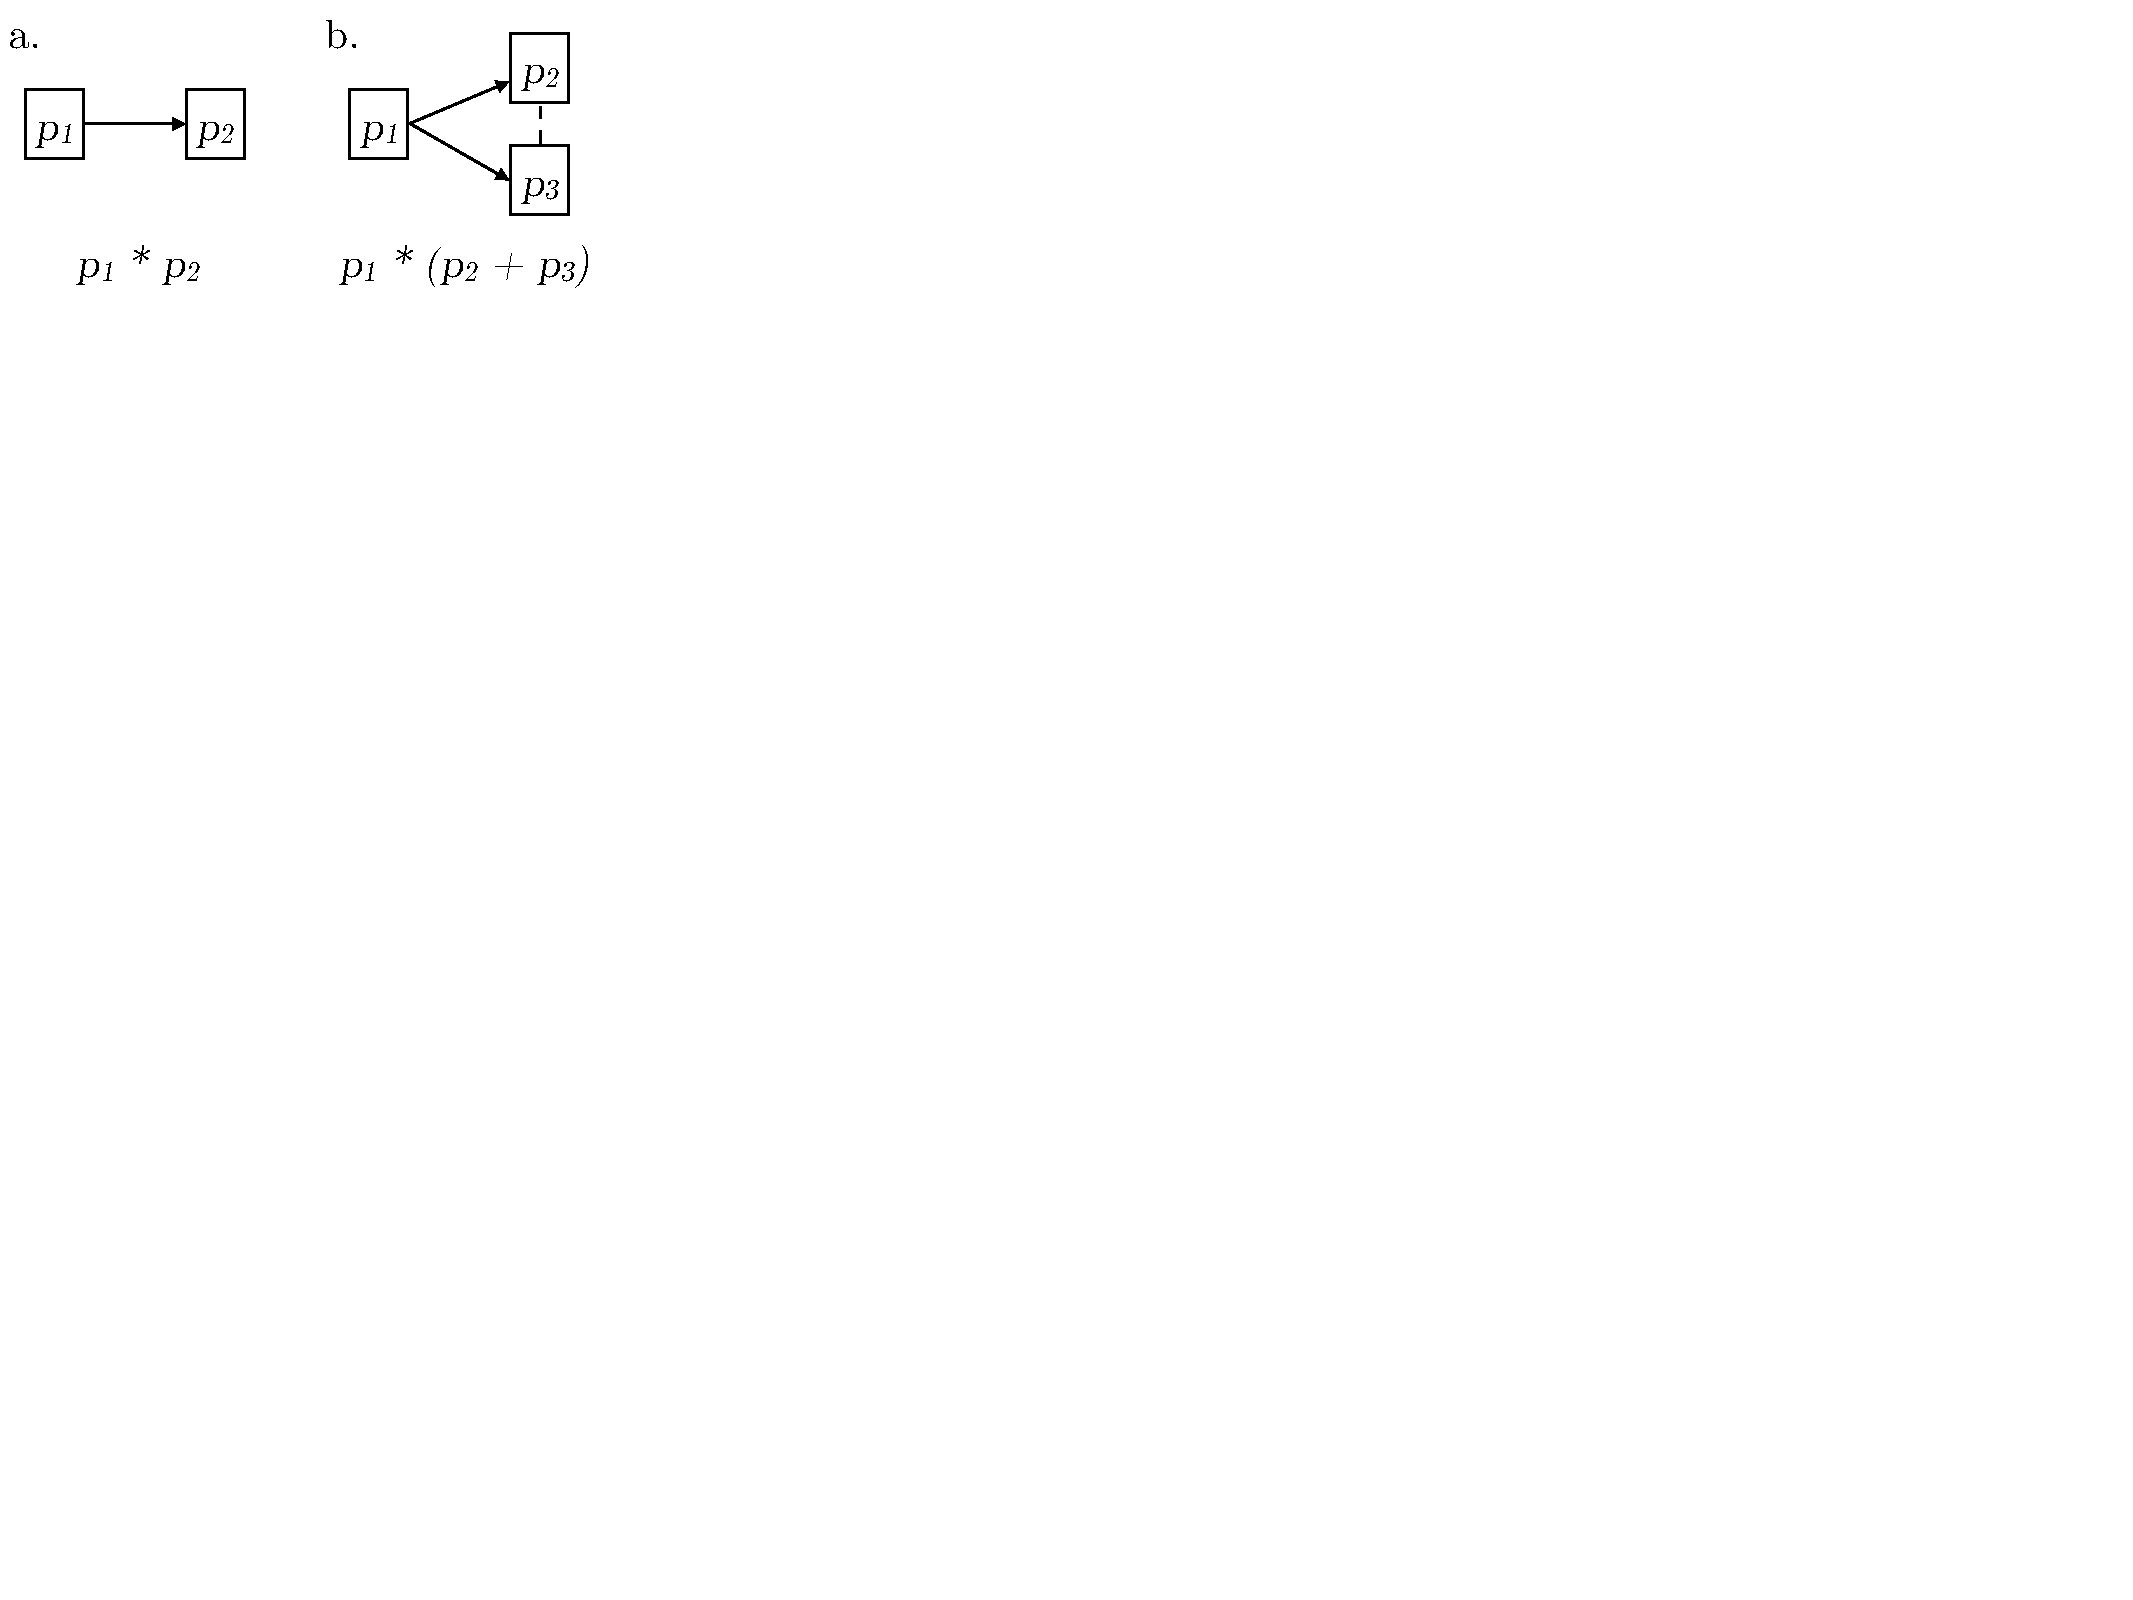
\includegraphics[clip, trim=0in 9.2in 10.25in 0in, width=1.75in]{figures/serial-and-parallel-composition.pdf}
    \vspace{-2mm}
    \caption{a. $p_1$ and $p_2$ composed in serial. b. $p_2$ and $p_3$ composed in parallel.}
    \label{fig:serial-and-parallel-composition}
    \vspace{-2mm}
\end{figure}

\para{The cvs serial composition operator:} Suppose we compose two pipelines $p_1$ and $p_2$ in serial to form the pipeline $p_{12}$, where pipeline $p_i$ has cvs $cvs_i$, inputs $m_{ij} \in M_i$, and where $p_2$'s $w$ bit composition header input is given the special label $c$.

The cvs $cvs_{12}$ contains a cv $cv_{12}$ for each pair of cv $(cv_1, cv_2)$ in $cvs_1$ and $cvs_2$'s cross product. The value of cv $cv_{12}$ for a given subset of inputs $S_{12} \subseteq M_{12}$, where $S_1 = M_1 \cap S_{12}$ and $S_2 = M_2 \cap S_{12}$ is:

\begin{center}
$min[cv_1[S_1] + cv_2[S_2], w + cv_2[S_2], cv_2[S_2, c]]$
\end{center}

\vspace{3mm}
\textit{Proof:} First, we prove that there is a cv $cv_{12}$ for every $(cv_1, cv_2)$ pair. Each cv in a pipeline's cvs represents a path through that pipeline. When $p_1$ and $p_2$ are composed in serial, any path through $p_1$ followed by a path through $p_2$ constitutes a valid path through $p_{12}$ which requires a unique cv.

Next, we prove that the value of $cv_{12}$ for a given $S_{12}$ presented above is correct. Happily, we can prove this very simply by considering $p_{12}$'s paths' dfgs.

Let us label the path that a given $cv_{i}$ measures $path_i$, $path_i$'s dfg $G_i$, and $G_i$'s output node $out_i$. When we compose $path_1$ and $path_2$ to form $path_{12}$, we conceptually link $out_1$ to $path_2$'s composition header $c$. We can therefore build $G_{12}$ from $G_1$ and $G_2$ by adding an edge between $out_1$ and $c$ with capacity $w$ (Figure~\ref{fig:min-cuts-in-composed-pipeline}).

\begin{figure}[tbh]
    \centering
    \vspace{-1mm}
    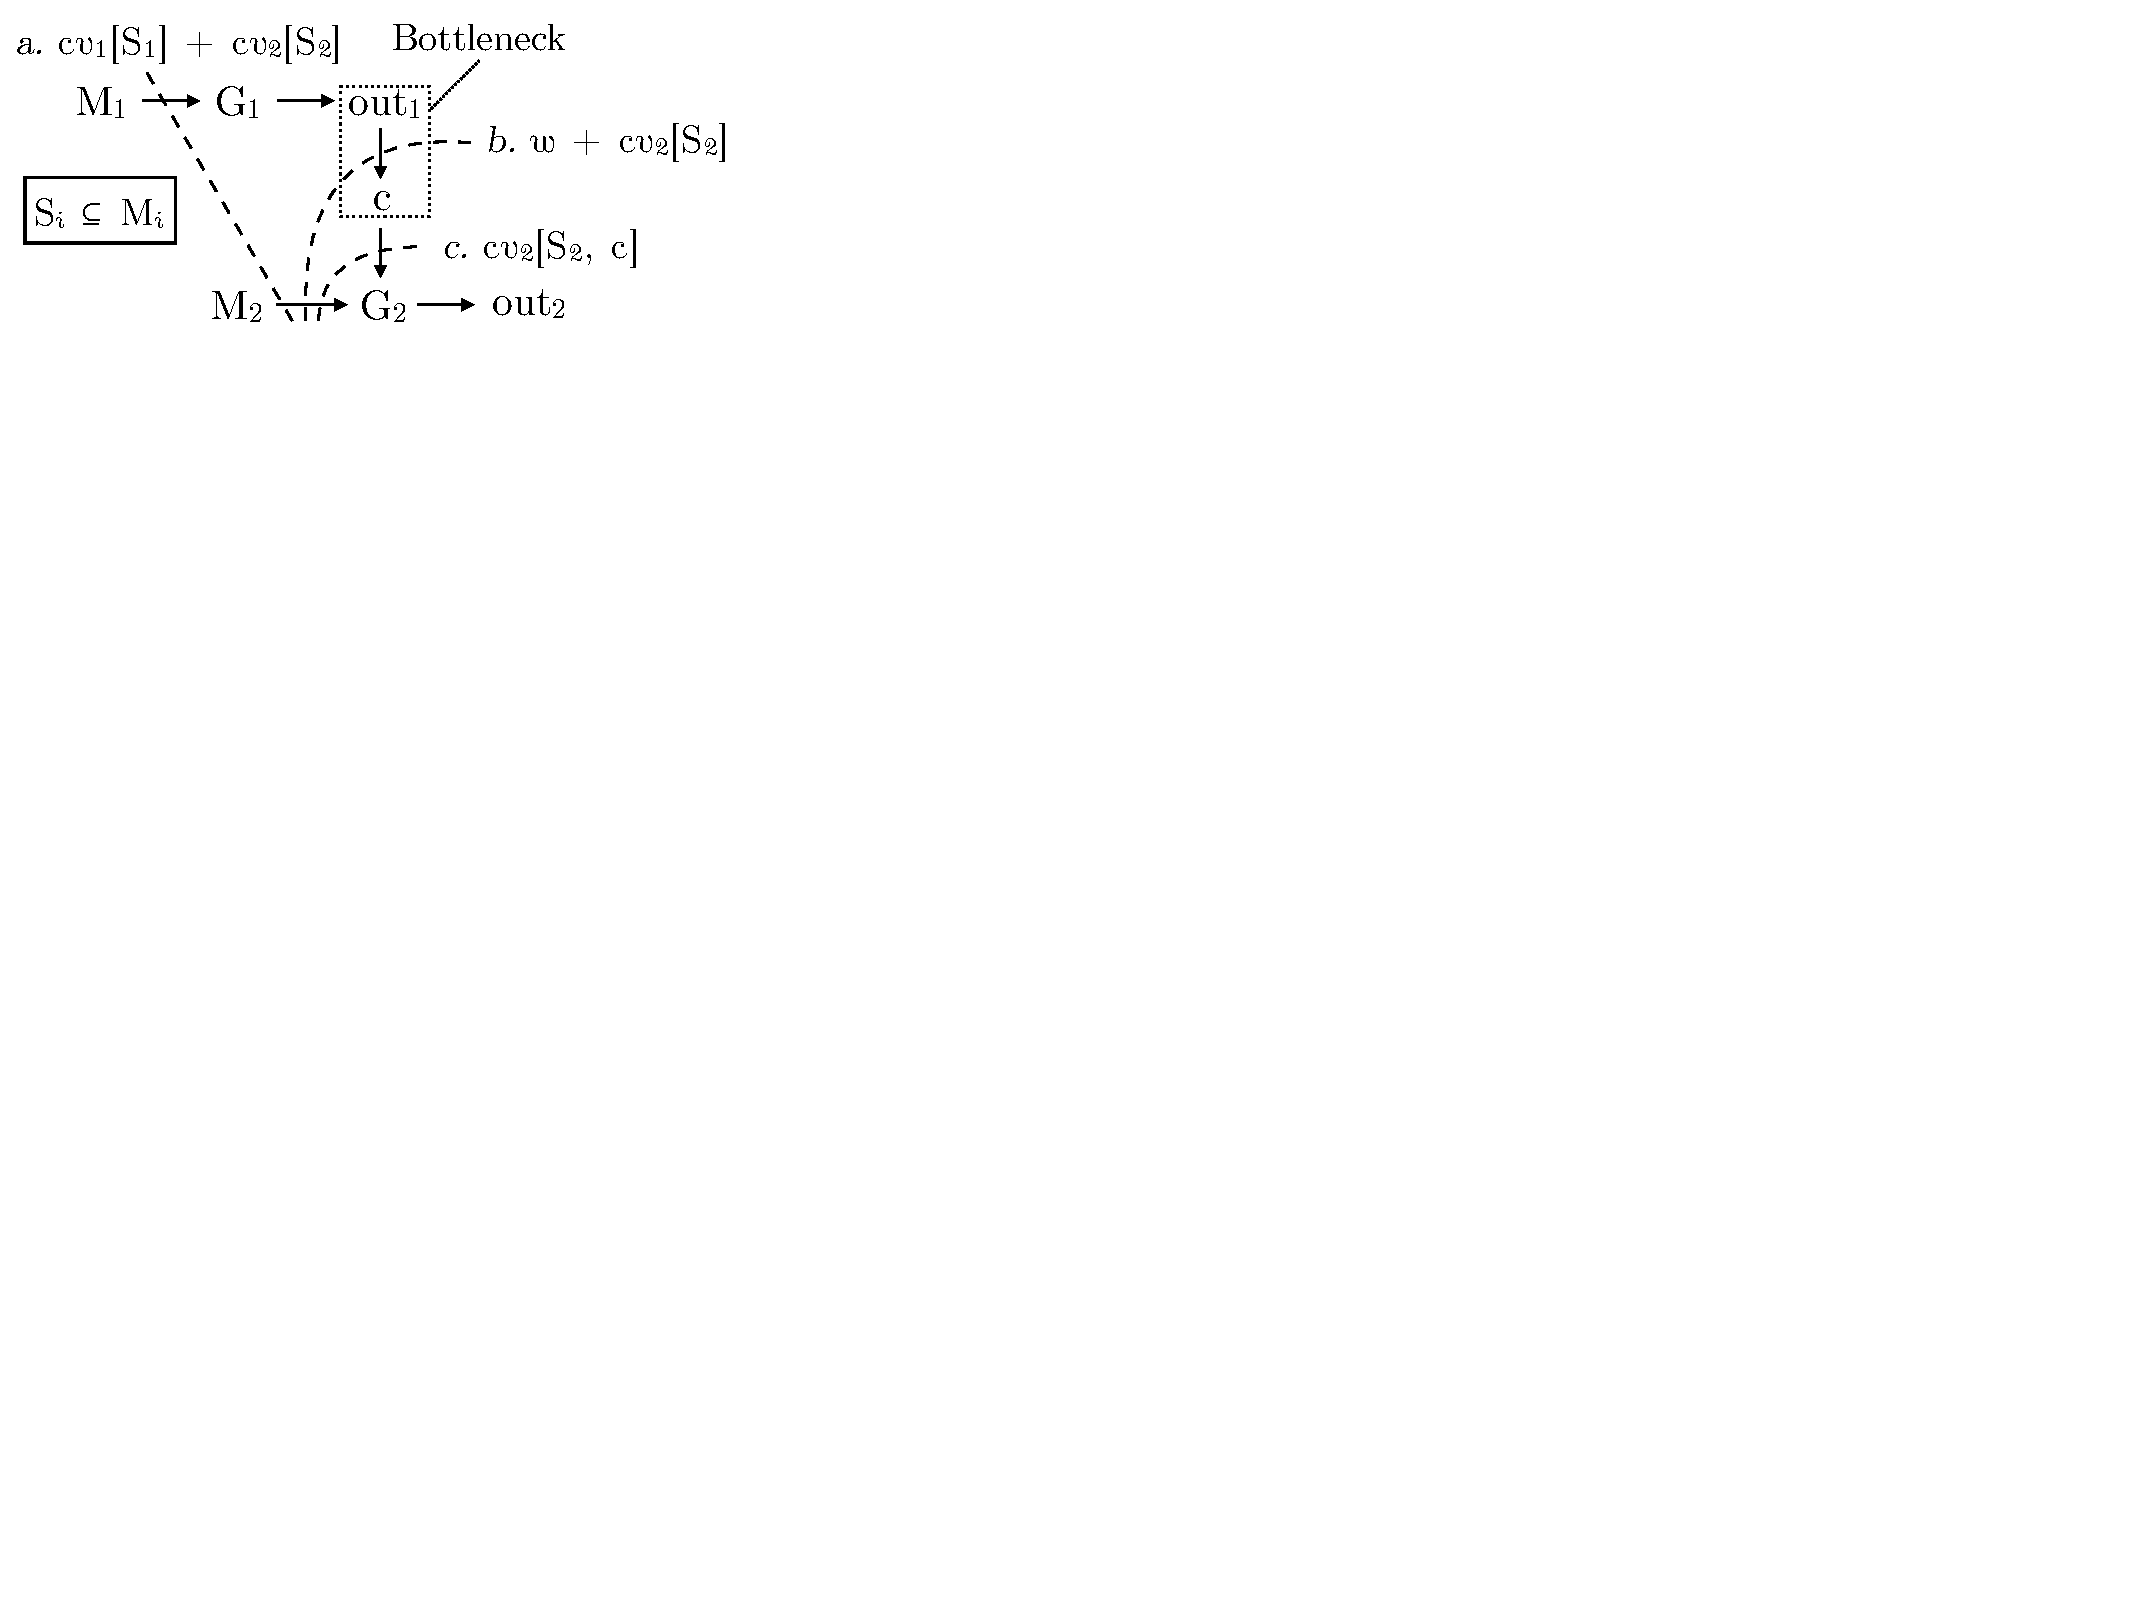
\includegraphics[clip, trim=0in 8.5in 9in 0in, width=2.5in]{figures/min-cuts-in-composed-pipeline.pdf}
    \vspace{-2mm}
    \caption{Min-cuts of $G_{12}$ a. before, b. through and c. after $G_{12}$'s bottleneck and their values.}
    \label{fig:min-cuts-in-composed-pipeline}
    \vspace{-2mm}
\end{figure}


Recall from Section~\ref{sec:pipeline-capacity-theorem} that a given $path_i$'s capacity for a given subset of inputs $cv_i[S_i]$ is the value of the min-cut separating $S_i$ from $out_i$ in $G_i$, and thus that $cv_{12}[S_{12}] = G_{12}.min-cut(S_{12}, out_2)$. The key to finding $S_{12}$'s min-cut is noticing that the edge $(out_1, c)$ forms a bottleneck in $G_{12}$ between $G_1$ and $G_2$, that this min-cut must thus either pass before, through or after this edge, and treating these three cases separately.

\vspace{3mm}
\textit{Case a. min-cut cuts before bottleneck:} The key to finding $S_{12}$'s min-cut in the case that it cuts before $G_{12}$'s bottleneck is noticing that such a min-cut must fully sever $S_1 = S_{12} \cap M_1$ from $out_1$. To see this, consider a min-cut that cuts before $out_1$ which does leave $S_1$ and $out_1$ partially connected. This min-cut must separate $out_1$ from $out_2$, but if $out_1$ and $out_2$ are separated we can decrease the value of the min-cut by leaving every edge between $S_1$ and $out_1$ uncut - a contradiction.

Given the above, in \textit{case a} the min-cut cuts through $G_1$ to sever $S_1$ from $out_1$ and then cuts through $G_2$ to sever any inputs in $S_{12}$ that $G_2$ contains - $S_2$ from $out_2$ (Fig~\ref{fig:min-cuts-in-composed-pipeline}a.) The value of this cut is simply $cv_1[S_1] + cv_2[S_2]$.

\vspace{3mm}
\textit{Case b. min-cut cuts through bottleneck:} In \textit{case b}, the min-cut cuts $(out_1, c)$ to separate $S_1$ from $out_2$, and then cuts through $G_2$ to sever $S_2$ from $out_2$ (Fig~\ref{fig:min-cuts-in-composed-pipeline}b.) The value of this cut is $w + cv_2[S_2]$.

\vspace{3mm}
\textit{Case c. min-cut cuts after bottleneck:} In \textit{case c} the min-cut only cuts $G_2$. To separate $S_1$ from $out_2$, the min-cut must sever both $c$ and $S_2$ from $out_2$. (Fig~\ref{fig:min-cuts-in-composed-pipeline}c.) The value of this cut is $cv_2[c, S_2]$.

\vspace{3mm}
Since the min-cut must either cut before, through or after the bottleneck the min-cut must take one of these three values, and thus we can find $cv_{12}[S_{12}]$ by finding $min[cv_1[S_1] + cv_2[S_2], w + cv_2[S_2], cv_2[S_2, c]]$ as above.

\para{The cvs parallel composition operator:} Suppose we compose two pipelines $p_1$ and $p_2$ in parallel to form the pipeline $p_{12}$, where pipeline $p_i$ has cvs $cvs_i$. $cvs_{12} = cvs_1 \cup cvs_2$

\vspace{3mm}
\textit{Proof:} When $p_1$ and $p_2$ are composed in parallel, incoming packets can take any path through either pipeline and thus every cv in $cv_1$ and $cv_2$ appears in $cv_{12}$.

\para{Pipeline capacity algebra properties:} Now that we have defined our composition operators and their actions on cvs, we show that these operators have certain useful properties: specifically, that they are associative and that $\times$ is distributive over $+$.

\vspace{3mm}
\textit{Distributivity of $\times$ over $+$:} The $\times$ operator can be characterized as a cross-product followed by an element-wise application of our $min[...]$ function, and the $+$ operator can be characterized as a simple union operation. Given these characterizations, $\times$ must be distributive over $+$ because both the cross product operator and any element-wise function are distributive over the union operator.

\vspace{3mm}
\textit{Associativity of $\times$:} Both the cross product of two sets and our $min[...]$ function are associative (proof omitted).

\vspace{3mm}
\textit{Associativity of $+$:} Trivially, the union of two sets is associative.

\subsection{Function transmission vector composition}
In the preceding section, we defined an algebra to calculate the joint cvs of composed pipelines. In this section, we turn our attention to calculating the joint tvs of composed functions. As before, we begin by defining function composition.

\vspace{3mm}
\textsc{Function composition:} Under function composition, one function's output is passed to another as an argument.

\para{Function tvs composition:} We now describe how we calculate the joint tvs of a composed function $f_{cmp}$ from the tvs of an initial function $f_1$ and a mapping from each of $f_1$'s parameters to the function $f_2$, ..., $f_n$, passed as an argument to that parameter (if applicable.)

\cleet{This is precisely the same as serial cvs composition - need to discuss how to merge the two.}
%\section{Compression of Capacity Vectors}

In this section, we first show the necessities of a set of capacity vectors for a pipeline by using a DAG to represent the pipeline. Each node in the DAG represents a table in the pipeline. If a table $t_i$ can jump to a table $t_j$ in the pipeline, then there is an edge between two nodes $n_i$ and $n_j$ which represents tables $t_i$ and $t_j$ respectively. Then, by the definition of capacity vector of a path in Section XXX, each path $p_i$ in the DAG should have a capacity vector $cv(p_i)$ to represent the capability for function computation.

Before diving into the compression of capacity vectors, we will give an analysis for capacity vectors for a pipeline. Specifically, we propose the following question: is it possible to only use a single capacity vector for a pipeline? In some cases, it is possible to use a single capacity vector since there are redundancies in capacity vectors. For example, TODO: two examples for merging and  inclusion.

Here, we define a concept of dominant table content $c_x$ as ...

\begin{lemma}
For a single table, there exists a dominant $c_x$ that dominates any other $c_i$.
\end{lemma}

Proof: ...

\begin{lemma}
For a path, there exists a dominant $c_x$ that dominates any other $c_i$.
\end{lemma}

Proof: ...

We can find that the definition of capacity vector of a path in Section XXX follows the proof of two lemmas. For a single table, it generates a single value $v$ for a set of matches $S$, and then it combines all these <$S$, $v$> entries for a path.

\begin{lemma}
For a pipeline with branches, there does not always exist a dominant $c_x$.
\end{lemma}
 
Proof: ...

Though the Lemma 3 answers the preceding question that it is not possible to only use a single capacity vector for a pipeline, as the example in Figure XXX, it is possible to do compression for a set of capacity vectors.

There are two kinds of compressions a set of capacity vectors: 1. Considering an unlimited size of tables, if a capacity vector $cv_i$ dominates another capacity vector $cv_j$, then we can only keep $cv_i$; 2. If two capacity vectors can be merged into one capacity vectors, then we can only keep the merged one. Since case 1 is very easy to identify, here we give an analysis for case 2. The difficulties of case 2 is that it is highly related to the structure of pipeline.

First, we have an obvious observation: If two paths have the same structure (including matches) after the branching point, then they can merge by doubling the value of equivalent class of matches in the branching point. For example, ...

Then, we extend the observation as the following: If two branch paths have the same capacity vector (including which register each entry uses) after the branching point, then they can merge by doubling the value of equivalent class of matches in the branching point. For example, ...

Using the extended observation, we give a recursive algorithm to compute and then compress capacity vectors for a pipeline as shown in Algorithm XXX. The algorithm ...

\begin{algorithm}
\If {$n.status$ = white}{
  \If {$n.nc$ = 0}{
    $n.nc$ $\gets$ ComputeCV($n$, null) \;
  }
  \ElseIf {$n.nc$ = 1}{
    $CV$ $\gets$ ComputeCV($n$, dfs($n.child$)) \;
    \If {$n.ta$ = false}{
      $n.nc$ $\gets$ $CV$ \;
    }
    \Else{
      $n.nc$ $\gets$ Merge(ComputeCV($n$, null), $CV$) \;
    }
  }
  \ElseIf {$n.nc$ $>$ 1}{
    New $CV$ \;
    \ForEach {node $c$ $\in$ $n.childs$}{
      $CV$ $\gets$ Merge($CV$, dfs($c$)) \;
    }
    $CV$ = ComputeCV(n, $CV$) \;
    \If {$n.ta$ = false}{
      $n.cv$ $\gets$ $CV$ \;
    }
    \Else{
      $n.nc$ $\gets$ Merge(ComputeCV($n$, null), $CV$) \;
    }
  }
  $n.status$ = black \;
}
\Return $n.cv$ \;
\end{algorithm}


\section{Performance Evaluation}
\label{sec:eval}

%Dynamic Datapath Configuration (DDC)
In this section, we will first demonstrate the benefits of \concept{} from two aspects: latency and total throughput, and then give the evaluation for the waypoints constraints computation part. All evaluations are run on an 3.5 GHz Intel i7 processor with 16 GB of RAM running Mac OSX 10.13.

\para{Methodology}: First we generate a random topology with 25 nodes and 50 edges. For every edge, we set two random values as its latency (5 - 10 ms) and bandwidth (5 - 10 Mbps). To model a flow in the topology, we randomly choose two nodes from the topology as the source and destination nodes of the flow. And a flow can have a sequence of nodes (other than its source and destination nodes) in the topology as its required ordered middleboxes for packet processing. (We add a constraint to the selection for these middlebox nodes that the number of neighbors of a middlebox node must equal to two as typically a middlebox does not have route selection capability, \ie, for any packet, it only has one output interface.) As a comparison of \concept{}, the traditional approach does not distinguish whether a middlebox is stateful or stateless. Therefore, when computing a path for a flow in the tradition way (\ie, do not apply \concept{}), it requires the path must pass through all the middleboxes in a correct order. And when computing a path for a flow in the \concept{} approach, we random choose a subset of its required middlebox nodes as stateful middleboxes since for \concept{} approach, stateful and stateless middleboxes are handled in different ways.

\para{Latency}: To show the benefits for the latency aspect, we consider a single flow and differentiate its number of required middleboxes. And the target is to find the optimal path to minimize the latency for the flow. Then, we compare the results (\ie, the minimal latency) between applying \concept{} and not.

\para{Total throughput}: To show the benefits for the total throughput aspect, we consider multiple flows and all flows have the same required middleboxes. We also differentiate the number of middleboxes. And the target is to find optimal paths that have maximum total throughput. Then, we compare the results (\ie, the maximum total throughput) between applying \concept{} and not.

\para{Execution time}: To evaluate the performance of \concept{}, we compare the execution time of the path computation to maximize total throughput for both approaches (\ie, applying \concept{} and not).

\para{Waypoints constraints computation}: To show the benefits of the waypoints constraints computation, we set a sequence of nodes in the topology as a flow's waypoints constraint. Then, we consider the minimal latency as system's objective and compare the results between applying the waypoints constraints computation and not (\ie, leading to excessive constraints). In the excessive constraints, all the middlebox nodes should be passed through before flow's waypoints.



\para{Results}: The results in Fig.~\ref{fig:eval12}(a) demonstrate that by using \concept{}, the latency can be reduced. Specifically, $F$ specifies the number of flows; $M$ specifies the number of required middleboxes for flows; $S$ specifies the number of stateful middleboxes for flows. As minimizing latency for a flow does not affect the results of other flows, the experiment only considers one flow scenario. From the results, we can see that without \concept{}, the latency of the flow grows up when the number of stateless middleboxes increases but if \concept{} is applied, the latency grows up only when the number of stateful middleboxes increases.

The results in Fig.~\ref{fig:eval12}(b) demonstrate that by using \concept{}, the total throughput can be increased. Specifically, when there are 5 flows and 3 middleboxes, the total throughput with \concept{} is around 3 times compared with that without \concept{}.

\begin{figure}[!htbp]
%\vspace{-2mm}
\centering
\begin{subfigure}{0.48\linewidth}
      \centering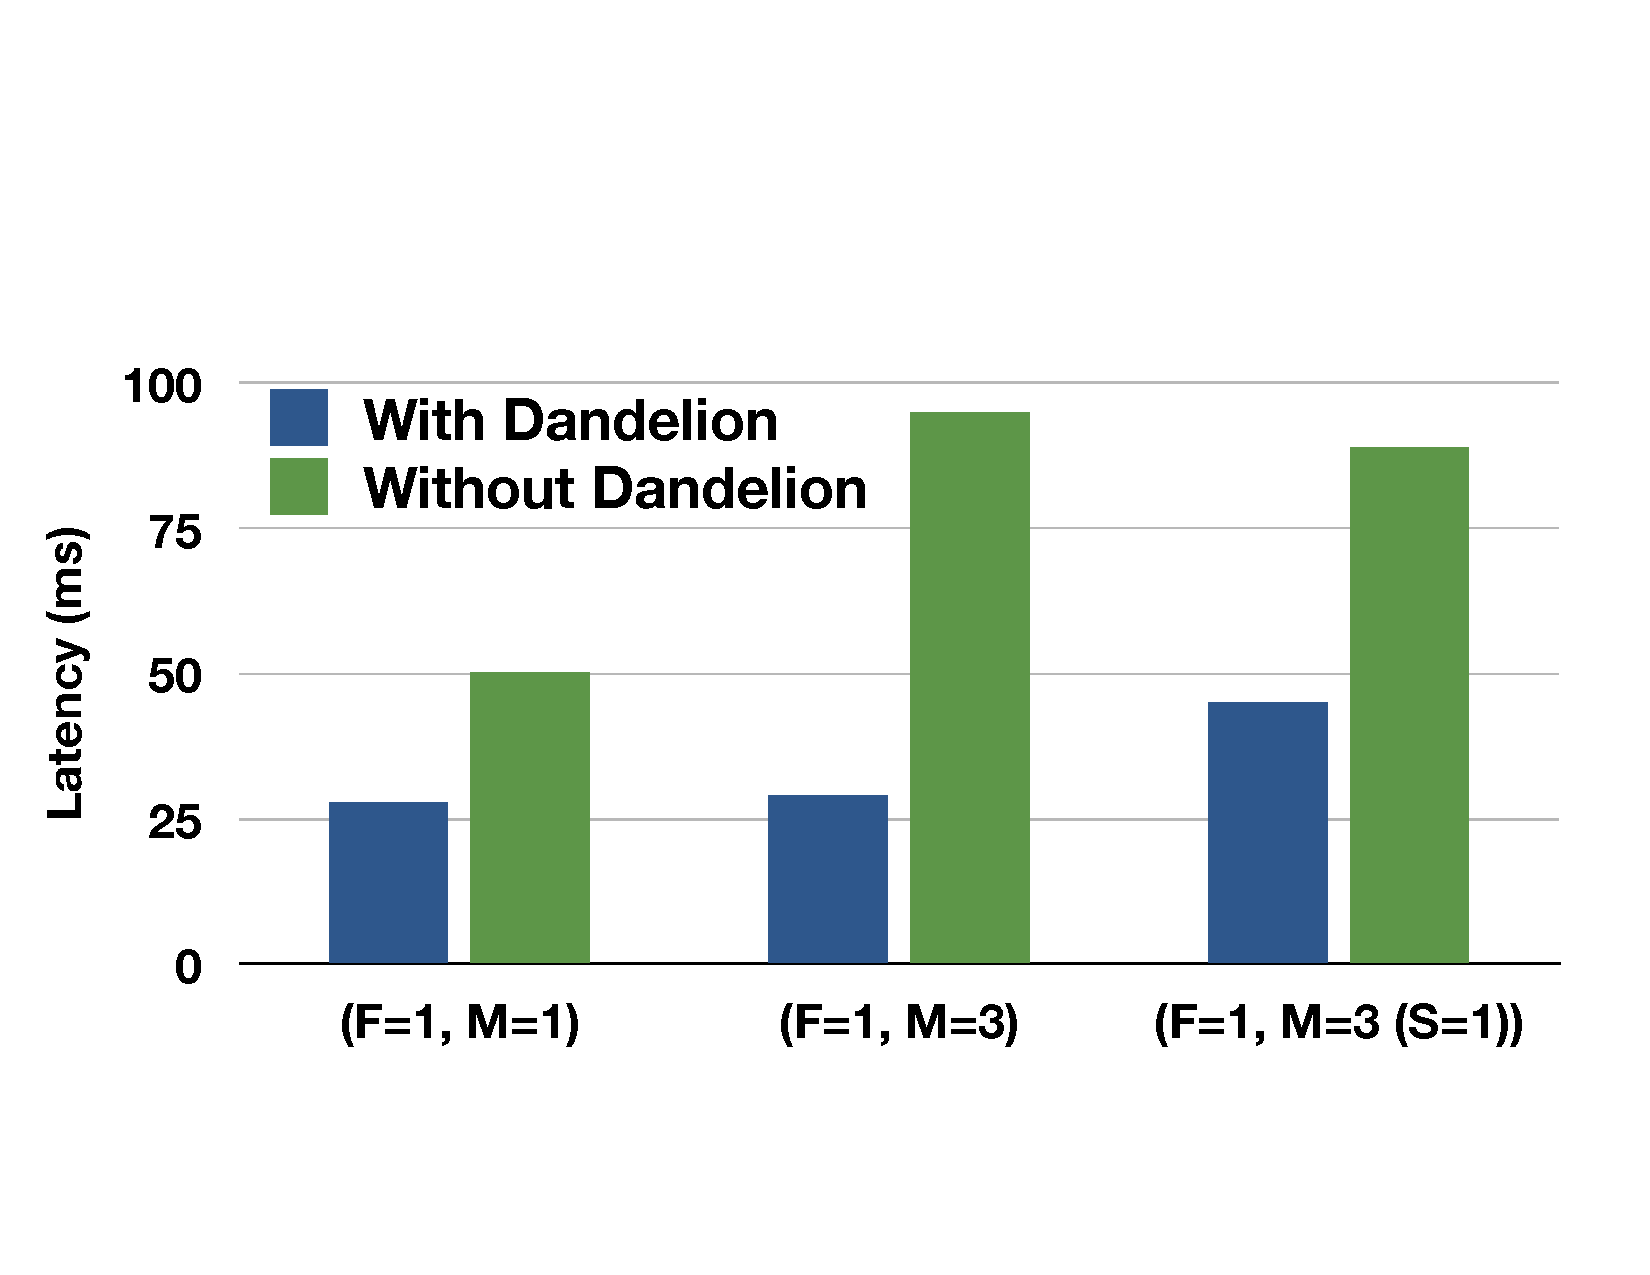
\includegraphics[width=\linewidth]{figures/ss-eval1.pdf}
      \caption{\label{fig:eval1} \small The latency for different scenarios.}
\end{subfigure}
%\hspace{0.03\linewidth}
\begin{subfigure}{0.48\linewidth}
      \centering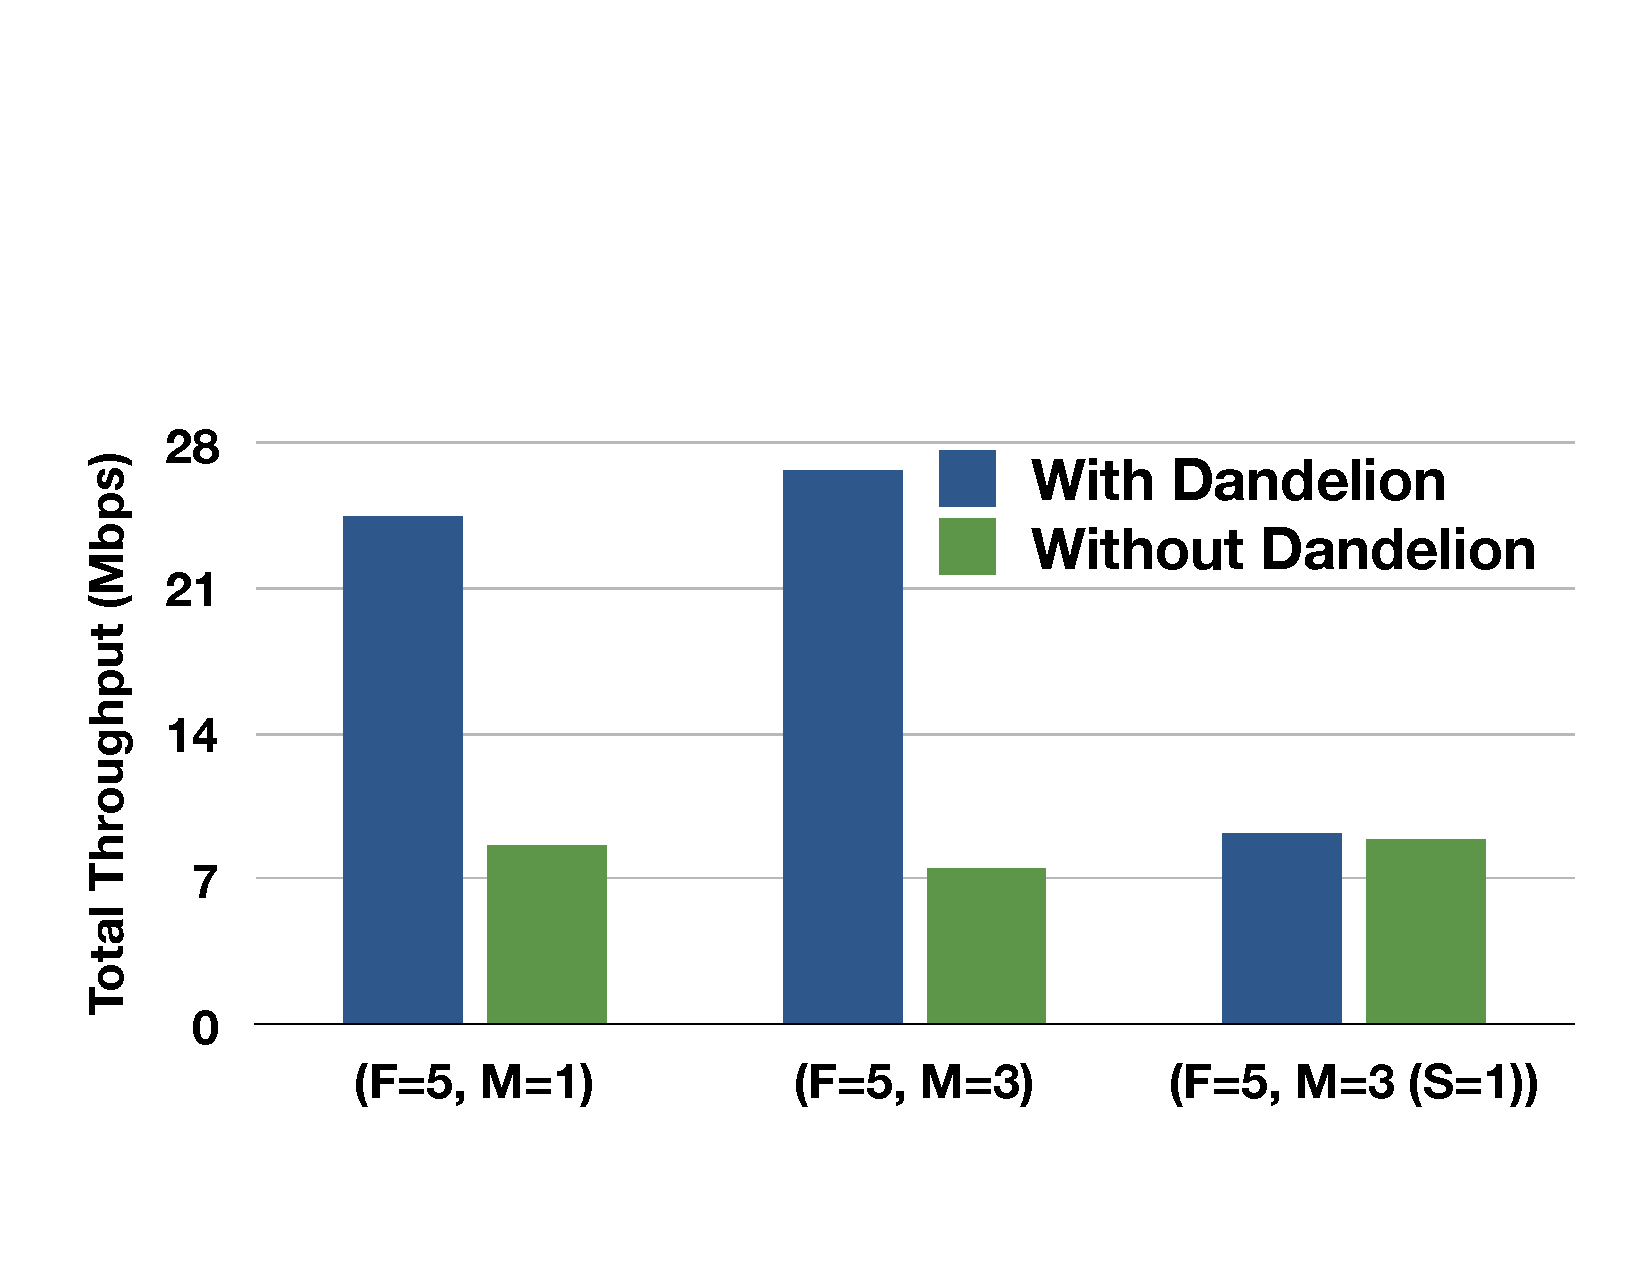
\includegraphics[width=\linewidth]{figures/ss-eval2.pdf}
      \caption{\label{fig:eval2} \small The total throughput for different scenarios.}
\end{subfigure}
\vspace{-2mm}
\caption{\small The benefits of \concept{} for latency and total throughput.}
%\vspace{-2mm}
\label{fig:eval12}
\end{figure}




%\begin{figure}[!htbp]
%%\vspace{-2mm}
%\centering
%\begin{subfigure}{0.8\linewidth}
%      \centering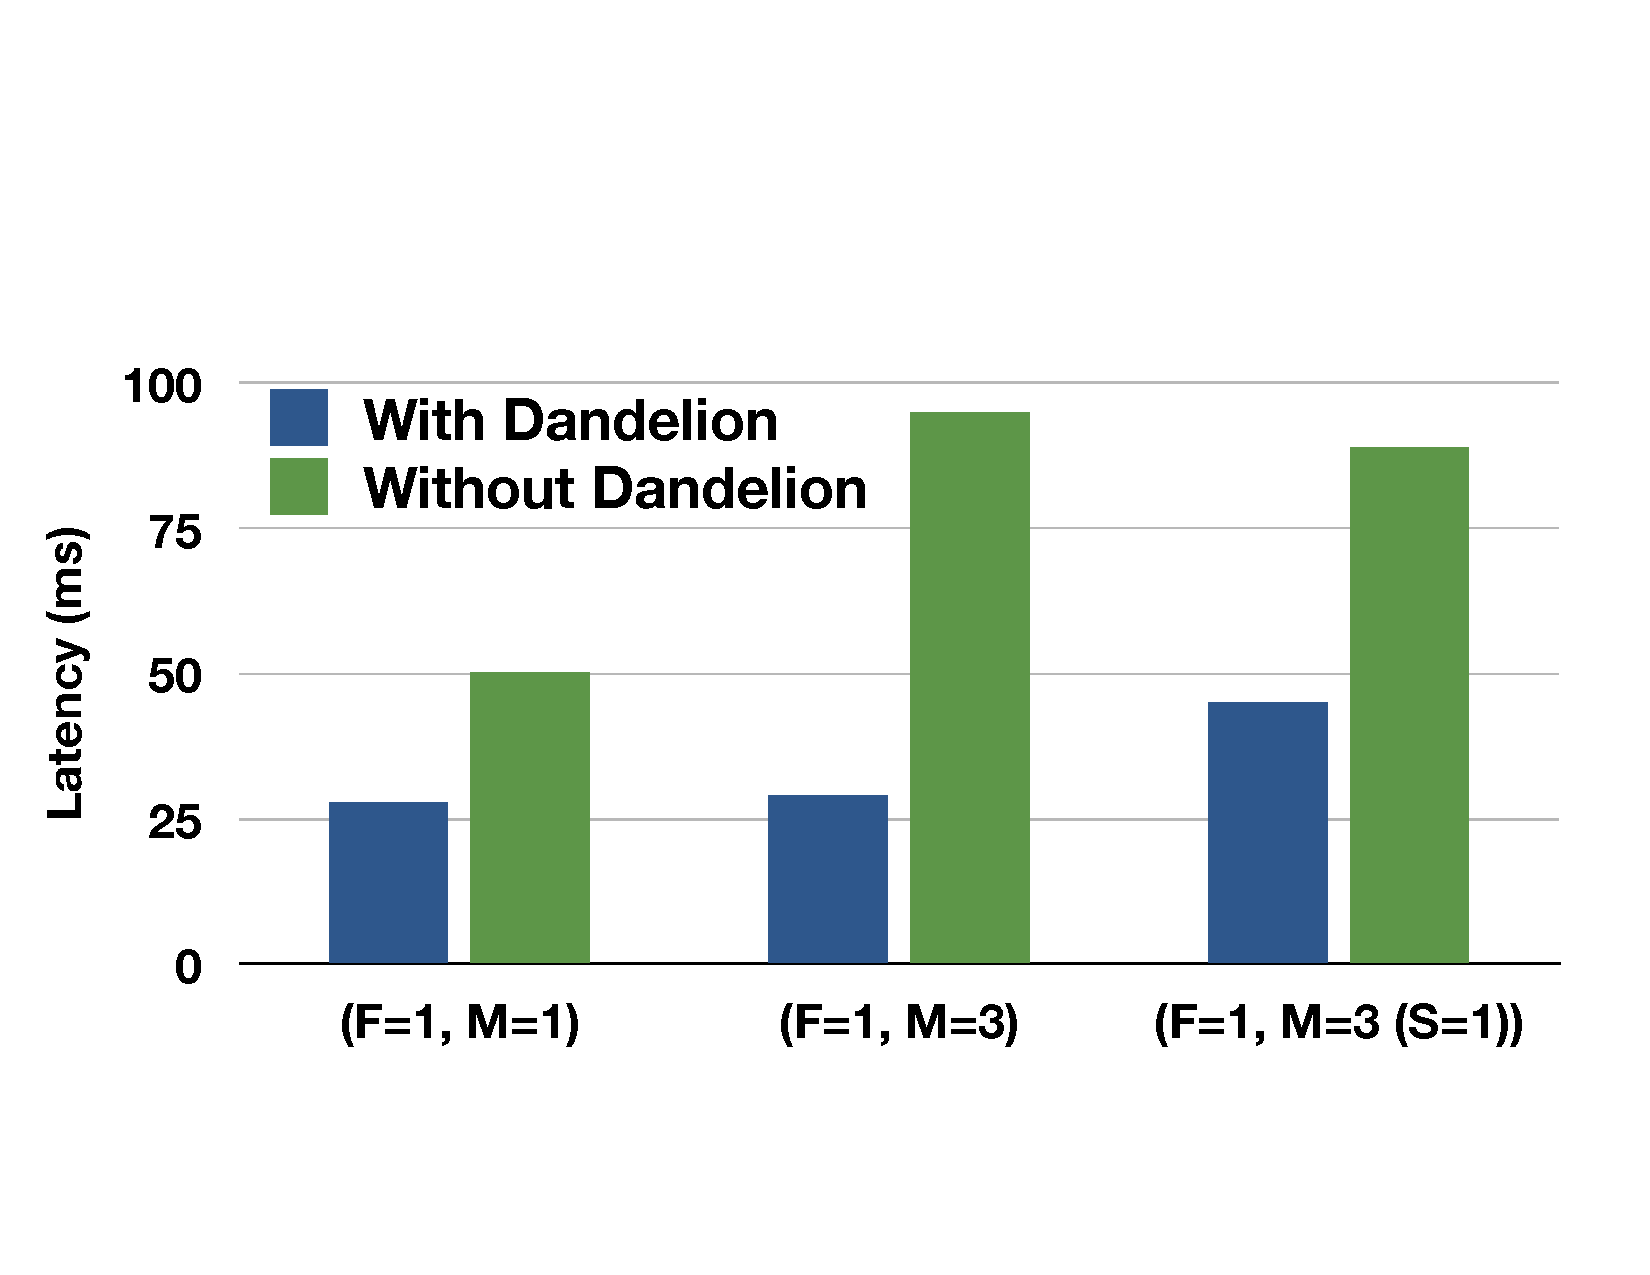
\includegraphics[width=\linewidth]{figures/ss-eval1.pdf}
%\end{subfigure}
%\hspace{0.03\linewidth}
%%\vspace{-2mm}
%%\caption{\footnotesize{The CDF of job latency local and remote jobs.}}
%\caption{\small The latency for different scenarios.}
%%\vspace{-2mm}
%\label{fig:eval1}
%\end{figure}




%\begin{figure}[!htbp]
%%\vspace{-2mm}
%\centering
%\begin{subfigure}{0.8\linewidth}
%      \centering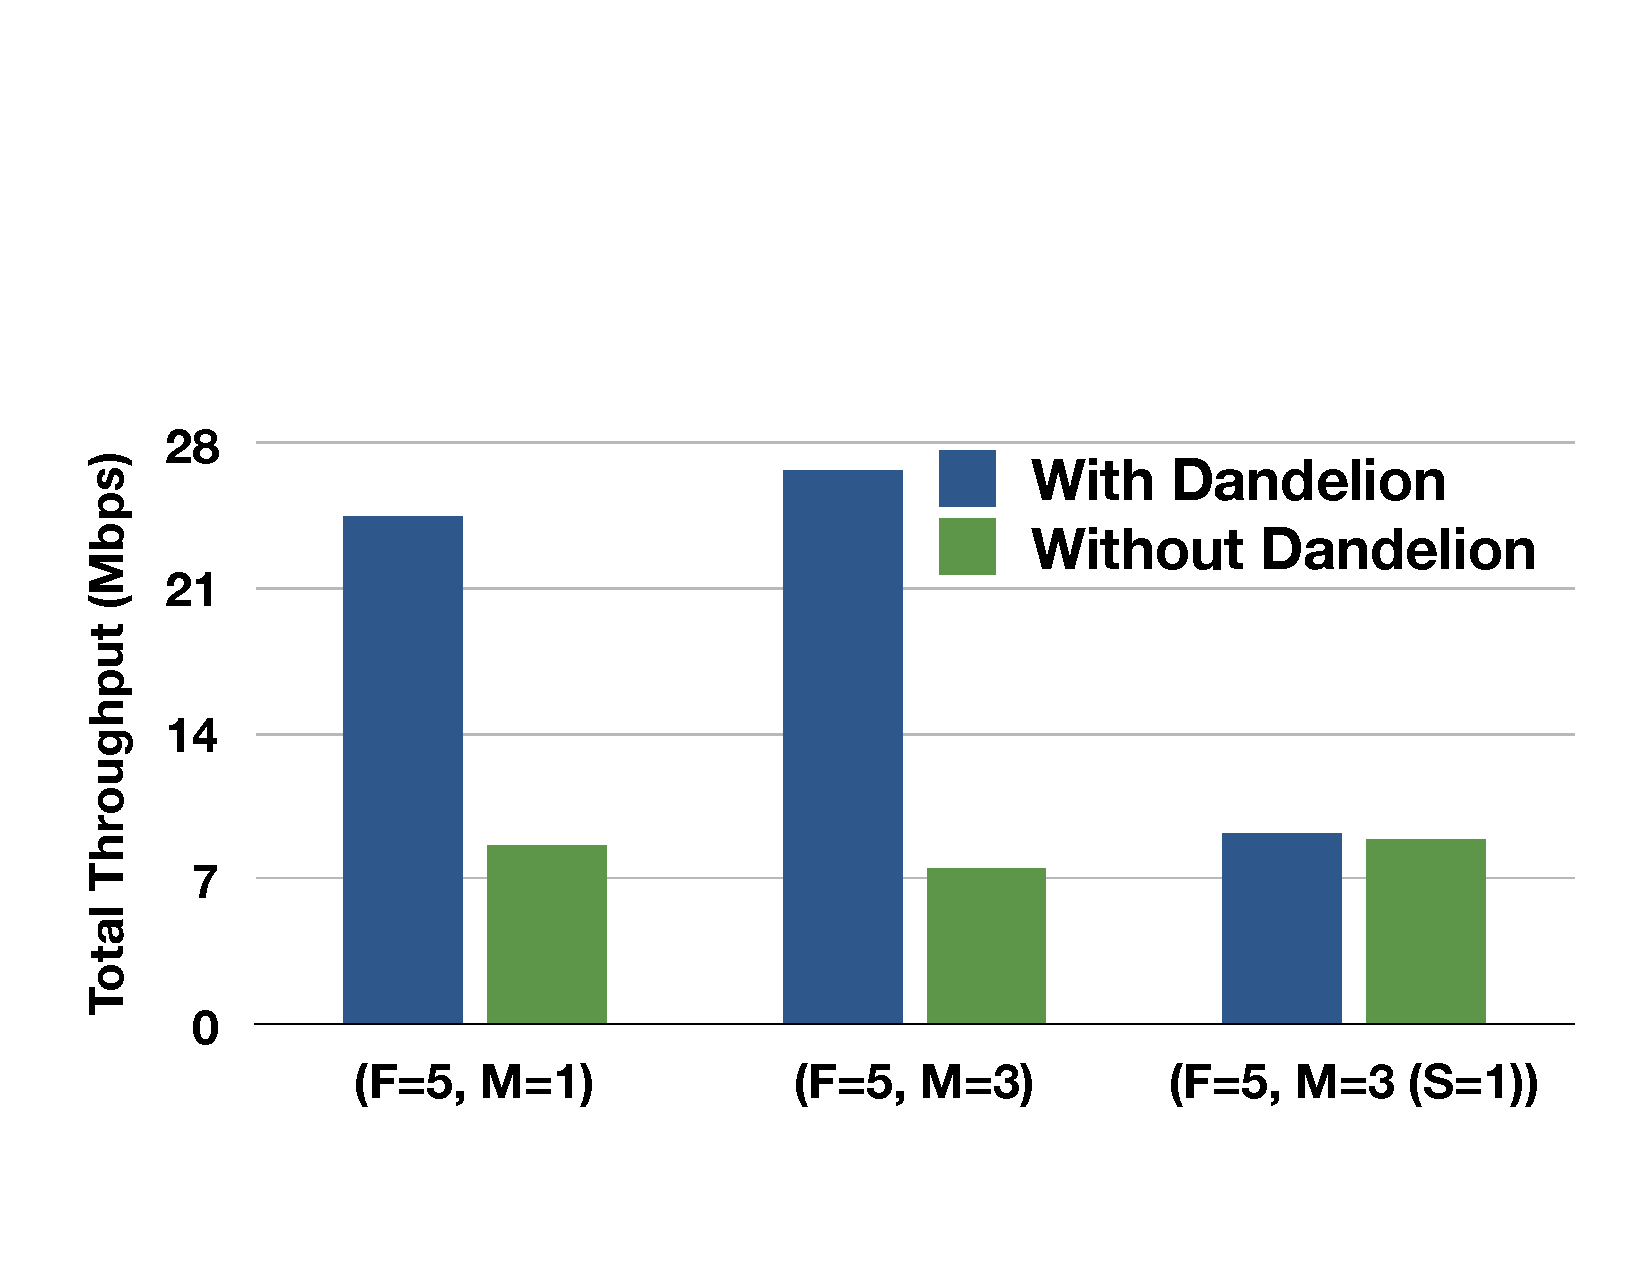
\includegraphics[width=\linewidth]{figures/ss-eval2.pdf}
%\end{subfigure}
%\hspace{0.03\linewidth}
%%\vspace{-2mm}
%%\caption{\footnotesize{The CDF of job latency local and remote jobs.}}
%\caption{\small The total throughput for different scenarios.}
%%\vspace{-2mm}
%\label{fig:eval2}
%\end{figure}

The results in Table~\ref{table:eval1} show the execution time of the path computation part to maximize total throughput. Since with \concept{}, the number of constraints is smaller than that without \concept{}, the execution time is also reduced (from 10.8 to 1.4 seconds when F=5 and M=3). 


\begin{table}[]
\footnotesize
\begin{tabular}{|l|l|l|l|}
\hline
             & \footnotesize(F=5, M=1) & \footnotesize (F=5, M=3) & \footnotesize (F=5, M=3 (S=1)) \\ \hline
With \concept{}    & 1.3 (s)    & 1.4 (s)    & 4.2 (s)          \\ \hline
Without \concept{} & 4.5 (s)    & 10.8 (s)   & 11.5 (s)         \\ \hline
\end{tabular}
\caption{\small The execution time of path computation to maximize total throughput for different scenarios.}
\label{table:eval1}
\end{table}


Fig.~\ref{fig:eval34} shows the latency with correct constraints (\ie, by
applying waypoints constraints computation) and with excessive constraints.
Specifically, the results in Fig.~\ref{fig:eval34}(a) consider that the
waypoints only have one node while Fig.~\ref{fig:eval34}(b) are for three nodes.
From the results, we can see the excessive constraints increase the latency,
\ie, lead to non-optimal path computation result. As the number of nodes
increases in the waypoints constraint, the latency with excessive constraints becomes larger.

\begin{figure}[!htbp]
%\vspace{-2mm}
\centering
\begin{subfigure}{0.48\linewidth}
      \centering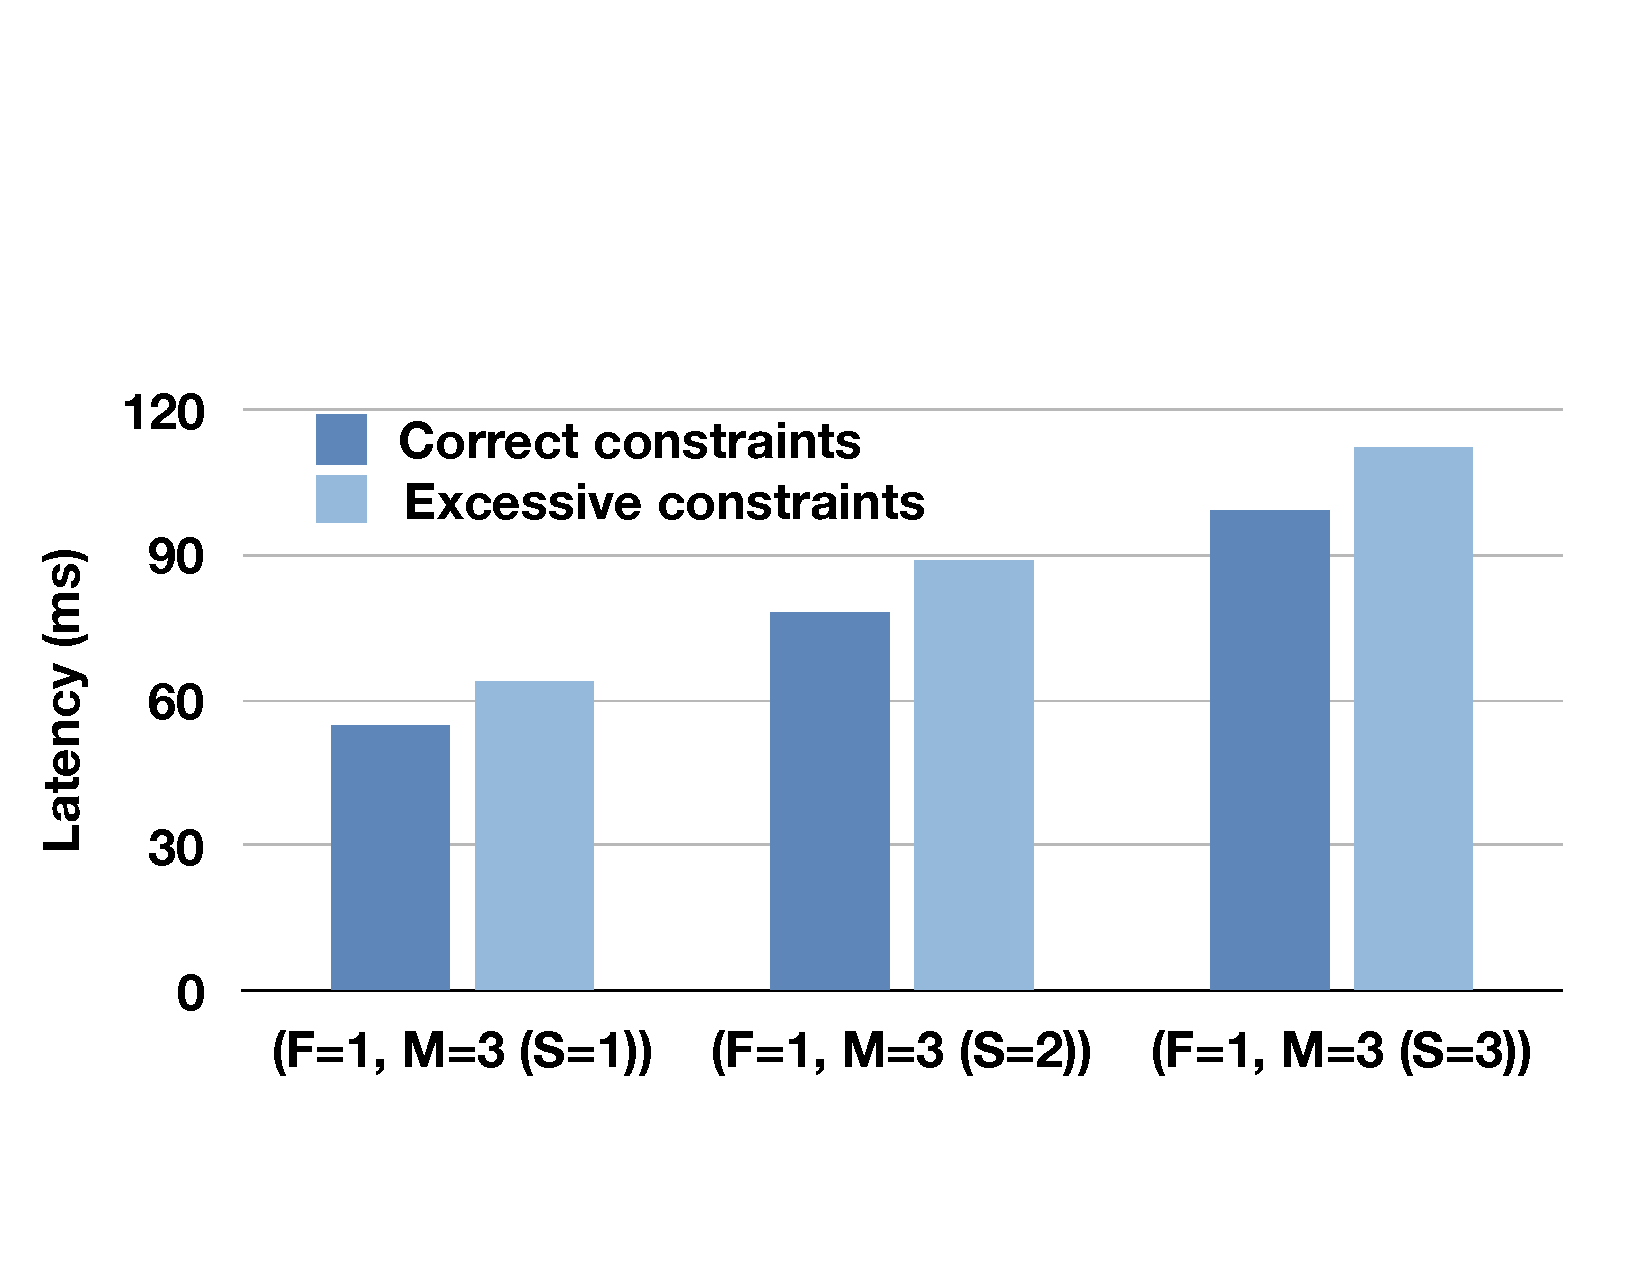
\includegraphics[width=\linewidth]{figures/ss-eval3.pdf}
      \caption{\label{fig:eval3} \small One node in waypoints constraint.}
\end{subfigure}
%\hspace{0.03\linewidth}
\begin{subfigure}{0.48\linewidth}
      \centering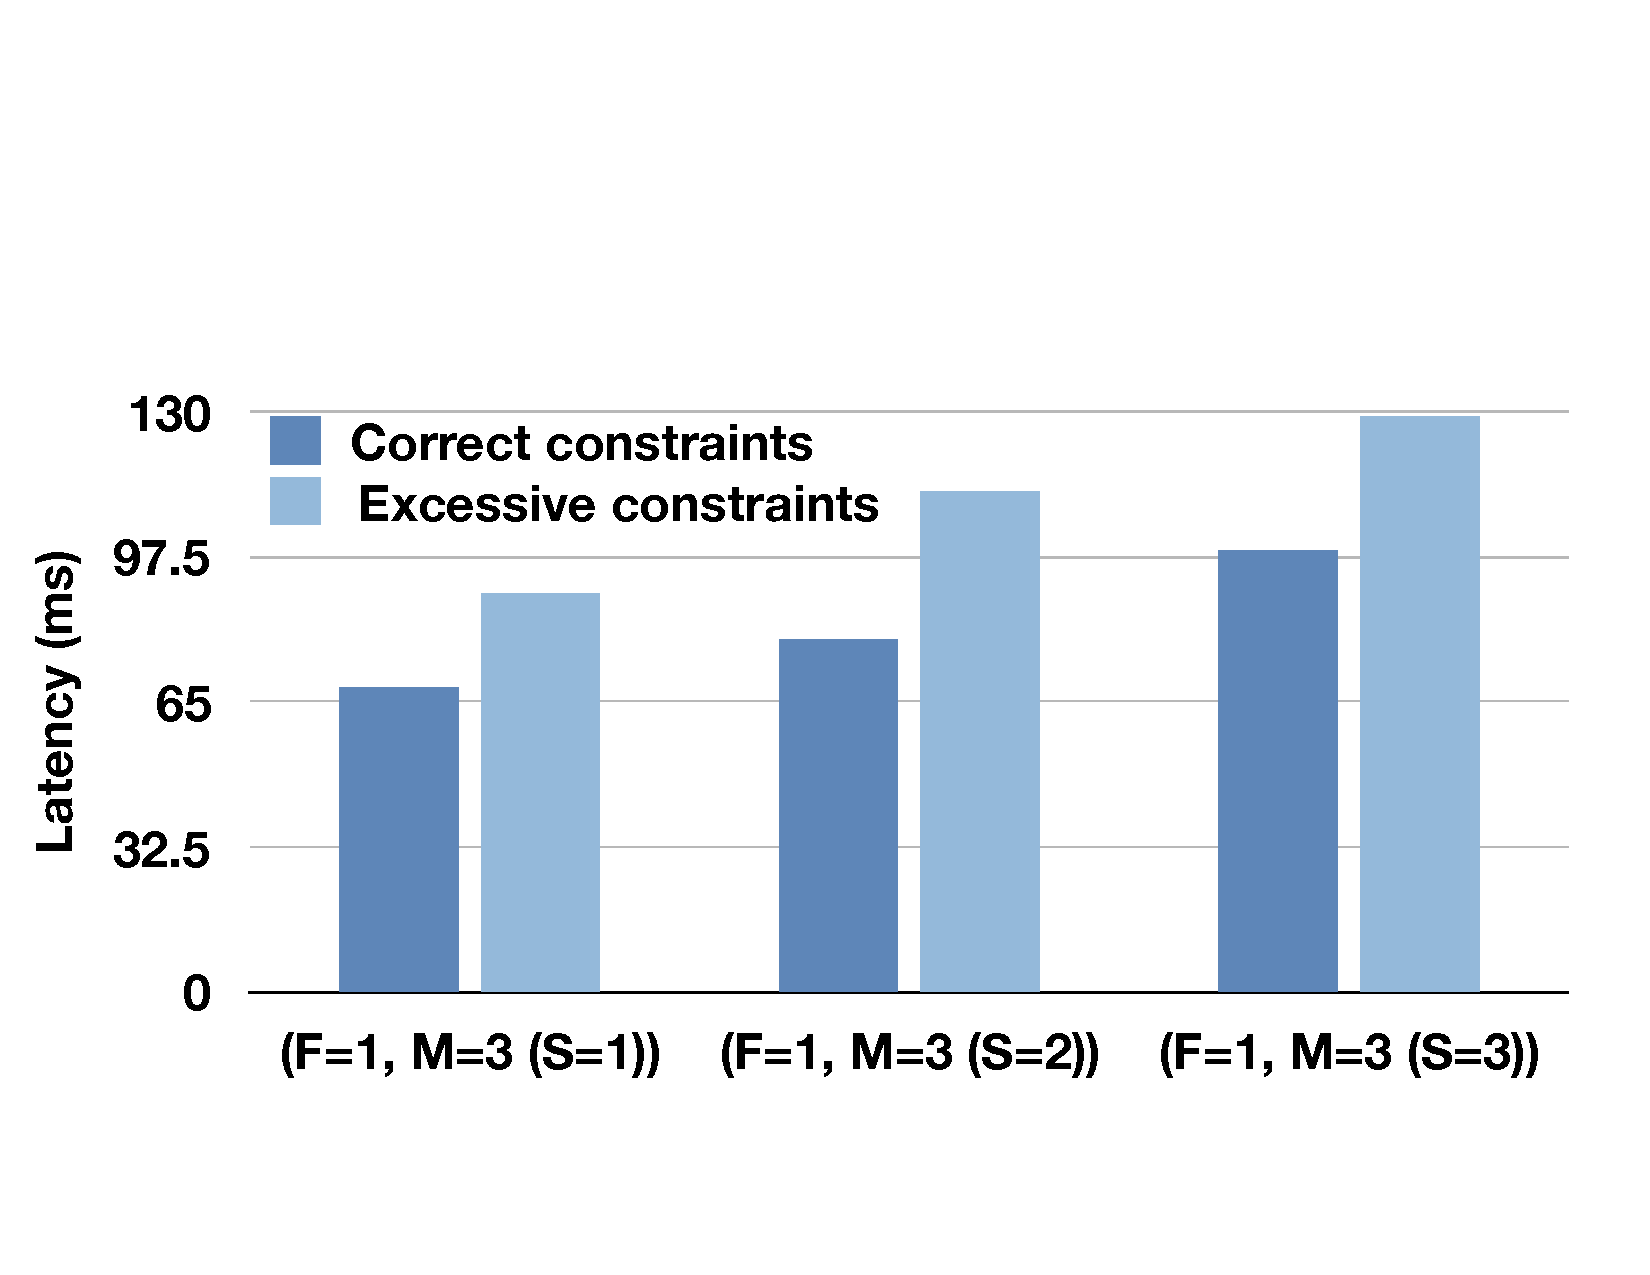
\includegraphics[width=\linewidth]{figures/ss-eval4.pdf}
      \caption{\label{fig:eval4} \small Three nodes in waypoints constraint.}
\end{subfigure}
\vspace{-2mm}
\caption{\small The latency with different waypoints constraints.}
%\vspace{-2mm}
\label{fig:eval34}
\end{figure}



%
%
%
%
%
%In this section, we will evaluate the proposed RSP design from two aspects: the execution time of pipeline design and the number of flow rules of the generated pipeline. All evaluations are run on an 3.5 GHz Intel i7 processor with 16 GB of RAM running Mac OSX 10.13.
%
%\subsection{Execution time}
%
%\para{Methodology}: Based on the analysis of the optimal pipeline design, we consider the following simple pipeline design algorithm: Given a DFG and $k$, recursively apply the source vertices selection $k-1$ times on the DFG to enumerates all the possible hardware pipelines. For the evaluation of both RSP and the unrolling approach, we randomly generate the DFG as the following: For the RSP, we change the number of software pipelines in the RSP (\ie, the number of iterations of the loop, $n$) and the number of vertices in the DFG of each pipeline (given the number of vertices, randomly generate the dataflow graph); For the unrolling approach, for each generated software pipeline in the RSP, we remove several vertices randomly. Then, we compare the execution time of RSP approach with the unrolling approach. Note that the complexity of enumerating all the possible pipelines equals to find the optimal pipeline as we do not consider the merging algorithm.
%
%%Then we evaluate the execution time of both RSP design and the unrolling approach. Specifically, for the evaluation of the RSP design, we change the number of software pipelines in the RSP and the number of vertices in the DFG of each pipeline (given the number of vertices, randomly generate the dataflow graph). To model the unrolling approach, for each pipeline in the repeated pipeline, we remove several vertices randomly. Then, we compare the execution time of repeated pipeline approach and the unrolling approach.
%
%\para{Result}: The result is shown in Figure~\ref{fig:eval1}. The horizontal axis specifies the number of iterations of the loop ($n$). The difference of Figure~\ref{fig:eval1-a} and Figure~\ref{fig:eval1-b} is the number of vertices ($m$) in the DFG of each software pipeline (for the unrolling approach, it means the number before removing vertices randomly) where $m = 10$ in Figure~\ref{fig:eval1-a} and $m = 20$ in Figure~\ref{fig:eval1-b}. And all the pipeline designs have the same $k$ as the limited number of flow tables where $k=10$. From the results, we can see that the RSP approach has smaller execution time compared (around 10 times when $n = 50$ and $m = 10$) with the unrolling approach when $k < n$. Note that when $n = 10$, both RSP and unrolling approach consider 10 software pipelines in the pipeline design, therefore, the execution time of both approaches is the same. And when $n = 100$, the execution time of unrolling is too large compared with the RSP approach.
%
%\begin{figure}[!htbp]
%%\vspace{-2mm}
%\centering
%\begin{subfigure}{0.47\linewidth}
%      \centering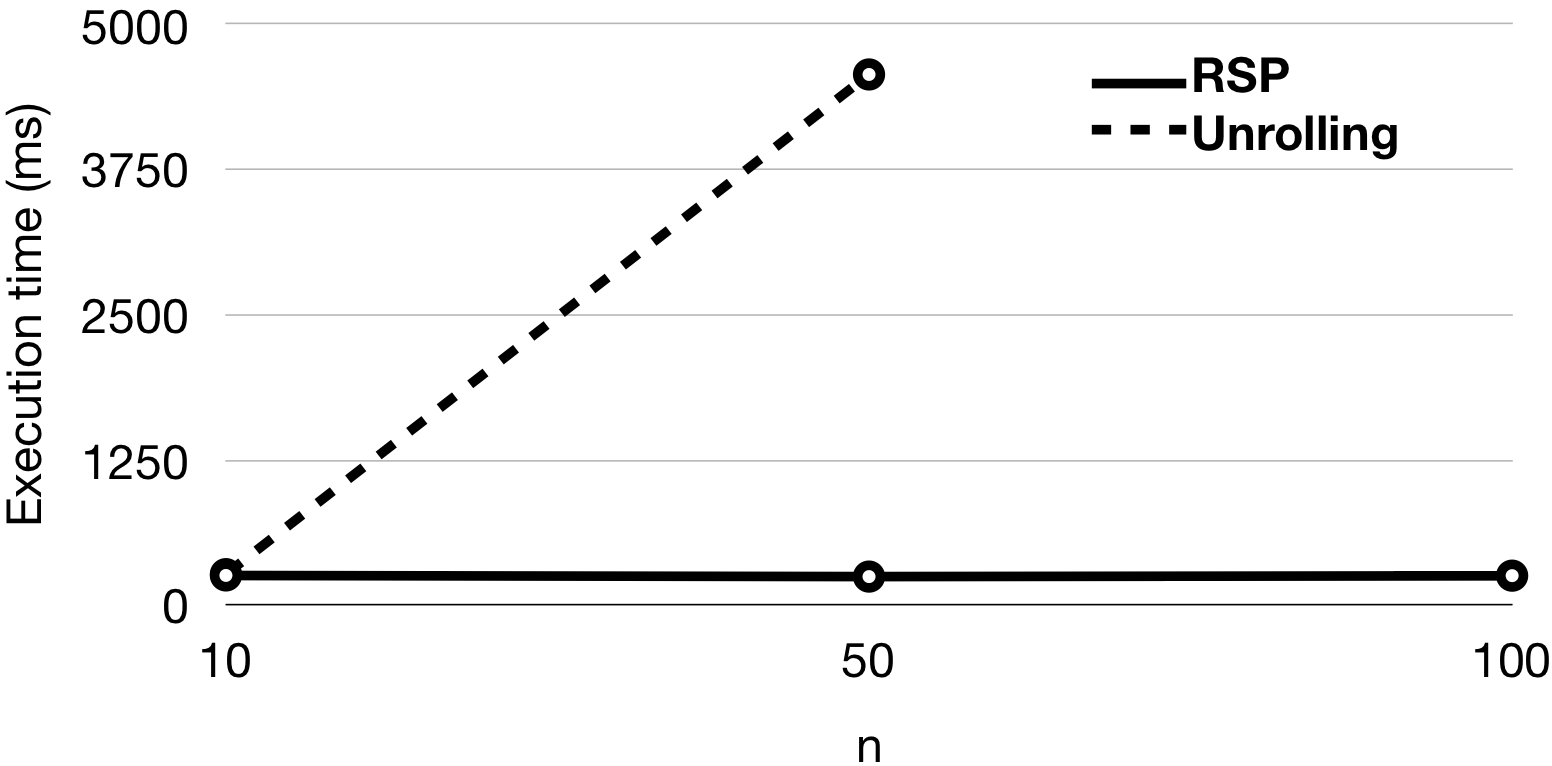
\includegraphics[width=\linewidth]{figures/lp-70.png}
%      \caption{\label{fig:eval1-a} \small $m$ = 10.}
%\end{subfigure}
%\hspace{0.03\linewidth}
%\begin{subfigure}{0.47\linewidth}
%      \centering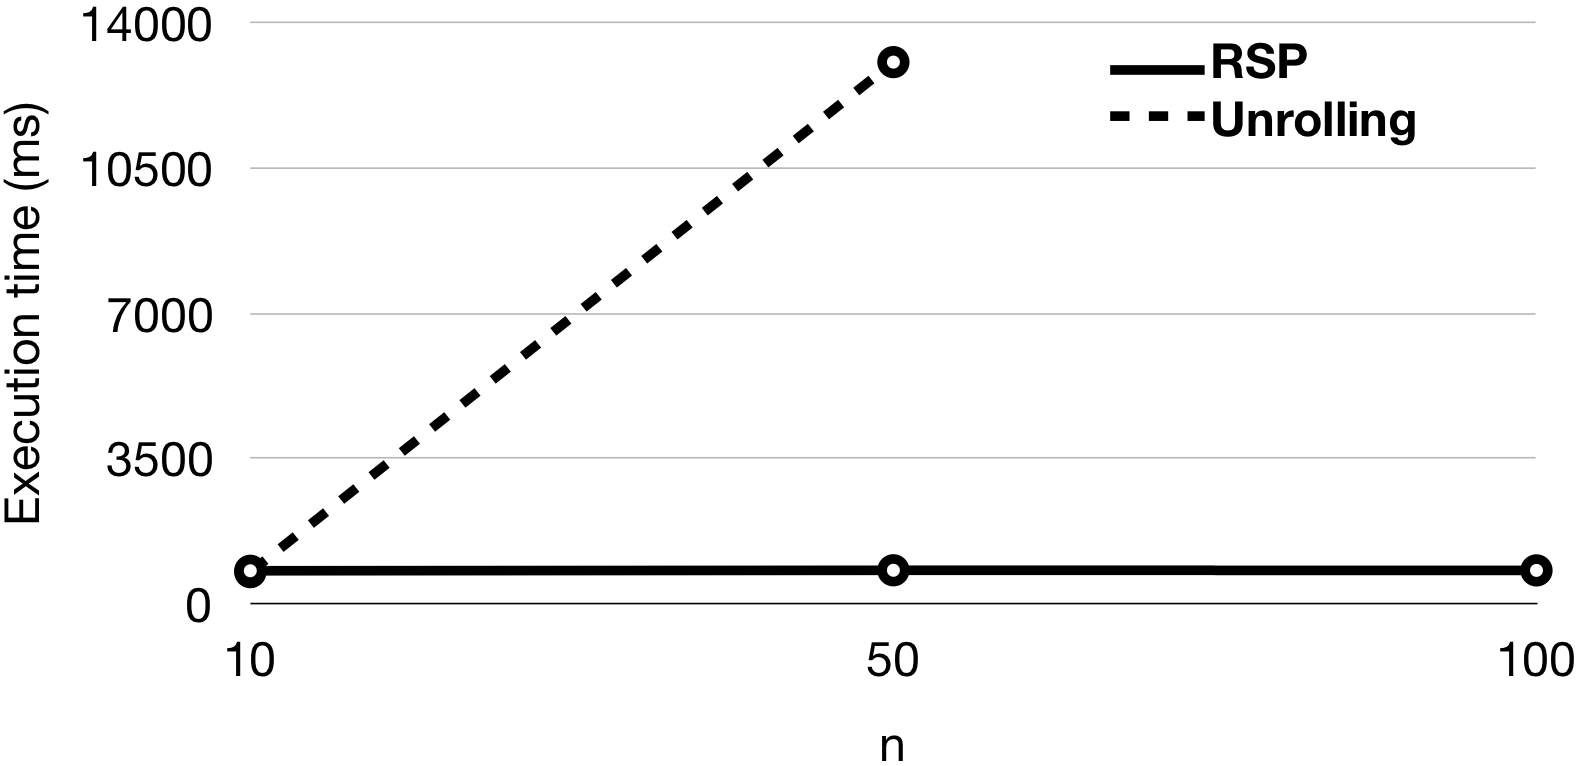
\includegraphics[width=\linewidth]{figures/lp-71.png}
%      \caption{\label{fig:eval1-b} \small $m$ = 20.}
%\end{subfigure}
%%\vspace{-2mm}
%%\caption{\footnotesize{The CDF of job latency local and remote jobs.}}
%\caption{\small The execution time of two approaches by changing the number of iterations ($n$) and the number of vertices ($m$).}
%%\vspace{-2mm}
%\label{fig:eval1}
%\end{figure}
%
%\subsection{Number of Flow Rules}
%
%\para{Methodology}: To compute the number of flow rules, we assign each variable (\ie, the vertex of DFG) the size of domain (\ie, the number of available values for the variable) randomly. Specifically, for the source vertices in the DFG of each software pipeline, we set the value from 100 to 200. And for the internal vertices in the DFG, we set the value from 10 to 20. This is because for the source vertices, they may represent packet fields which should have a larger range of values compared with internal variables in the program. Also, given a flow table, the computation of number of flow rules equals to the product of the size of domain of all the input variables. For example, a flow table consists of three input variables and their size of domain are 120, 10, 10 respectively, then the number of flow rules of the table is 12000. The definitions of $n$ and $m$ remain the same as the evaluation of execution time. We compare the number of flow rules of RSP design with the black-box approach (\ie, single table approach).
%
%\para{Result}: The result is shown in Table.~\ref{table:eval2}. As for the single table approach, the number of flow rules only depends on the first DFG of all software pipelines (which equals to the product of the size of domain of all the source vertices of the first DFG), so the values are the same for different $n$. From the result, we can find that the multi-table design can reduce the number of flow rules significantly compared with the single table approach. Also need to note that by the RSP approach, for each table, it may have a lot of unused flow rules. For example, the \codeword{while i in range(100)} statement can be viewed a flow table that matches \emph{i} and writes to \emph{i} with 100 flow rules (\ie, i = 0, 2, ..., 99), which has 99 unused flow rules when the table is the first table. Therefore, the number of flow rules can be reduced further by existing work which will not be discussed in this paper.
%
%\begin{table}[!htbp]
%\centering
%\begin{tabular}{|l|l|l|}
%\hline
%         & n =10, m = 10 & n = 50, m= 10 \\ \hline
%Single  & 3898434       & 3898434       \\ \hline
%RSP & 61856         & 224098        \\ \hline
%\end{tabular}
%\caption{\small The number of flow rules of the single table approach and the RSP approach.}
%\label{table:eval2}
%\end{table}
%


\section{Related Work}\label{sec:related-work}
\para{High level SDN Program Compilers:} Multiple systems that allow programmers to write SDN programs in high level languages and then compile such programs to flow table pipelines have been proposed over the last several years. Such systems are related to our work in that they examine the transformation of policy programs into switch flow tables. We group these systems into two categories: \textit{tier-less} and \textit{split-level}.

\textit{Tier-less} systems (\eg\ SNAP~\cite{SNAP}, FML~\cite{fml}, FlowLog~\cite{flowlog},  Maple~\cite{maple}), require programmers to specify forwarding behaviors as packet handling functions which are then used by the SDN controller to configure and update network state. Such systems pioneer our pipeline capacity theorem's notion of a \textit{program function} and are able to compile such functions to single pipelines. These systems, however, are unable to verify that submitted functions can be written to a given pipeline without physically carrying out the time consuming process of compilation, and cannot write programs to multi-pipeline networks.

\textit{Split-level} systems such as the Frentic family (\eg\ Frenetic~\cite{frenetic}, Pyretic~\cite{pyretic}) provide a two tiered programming model in which controller programs specify events of interest and then respond to these events when they occur by calculating new network policies. Again, such systems cannot verify that a given controller program's output can be written to the controller's switches' pipelines, although this paradigm falls outside of our pipeline capacity theorem's model as well.

\para{Pipeline specification languages:} There are some superficial similarities between pipeline specification languages (\eg\ P4~\cite{P4}, PISCES~\cite{PISCES}, Concurrent NetCore~\cite{ConcurrentNetCore}) and our pipeline capacity theorem, such as the analysis and guarantees that such languages provide about pipeline behavior. For example, Concurrent NetCore's type system ensures that any program used to populate a pipeline has certain properties, such as determinism, whilst PISCES's switch specification allows compilers to analyze pipelines and optimize their performance. We contend, however, that our capacity theorem attacks an entirely different space in pipeline analysis - guaranteeing pipeline properties or improving performance is qualitatively different to verifying whether compilation is possible.

%\para{Multi-switch network programming:} Our pipeline capacity algebra is related to other systems that facilitate multi-switch network programming, specifically DIFANE~\cite{DIFANE} and TableVisor~\cite{TableVisor}. These systems, however, focus on distributing a centrally specified flow table/flow table pipeline across a given network, whilst our algebra verifies that generic high level language programs can be written to it.

\para{Pipeline design:} Pipeline design schemes such as Jose et al.'s ``Compiling Packet Programs to Reconfigurable Switches''~\cite{Jose-et-al}, Sun et al.'s ``Software-Defined Flow Table Pipeline''~\cite{Sun-et-al}, FlowAdapter~\cite{FlowAdapter}, and Domino~\cite{Domino} are clearly related to our pipeline capacity theorem in that they examine pipeline layout design under hardware constraints. Jose et al., Sun et al., and FlowAdapter  however, focus on mapping logical lookup tables/flow table pipelines to physical tables whilst our pipeline capacity theorem focuses on generic programs, while Domino considers weaker hardware constraints (\eg\ limits on stateful operations at line-rate) than our work does.

衷心感谢导师 xxx 教授和物理系 xxx 副教授对本人的精心指导。他们的言传身教将使
我终生受益。

在美国麻省理工学院化学系进行九个月的合作研究期间,承蒙 xxx 教授热心指导与帮助,不
胜感激。感谢 xx 实验室主任 xx 教授,以及实验室全体老师和同学们的热情帮助和支
持!本课题承蒙国家自然科学基金资助,特此致谢。

感谢 \tongjithesis{},它的存在让我的论文写作轻松自在了许多,让我的论文格式规整漂亮了
许多。

\bibliographystyle{IEEEtran}
%\bibliographystyle{abbrv}
\bibliography{references}%[References]

%\bibliography{./references}
\appendix
\section{Proofs}
\label{sec:proofs}

\subsection{Proof of Pipeline Realization Theorem}

We now present proofs to verify our realization theorem. The structure of these proofs will be as follows. First, we define a mechanism to encode sufficient information about a given $M \in \mathcal{M}$ to fully execute a given $f$. Second, we show that a pipeline transmitting information internally using our encoding can realize an $f$ in $p$ given that $\kappa(p) \trianglerighteq \tau_G(f)$. Finally, we show that $\tau_G(f) > \tau(f)$, proving by extension that if $\kappa(p) \trianglerighteq \tau(f), f \rightrightharpoons p$. We omit a proof of Theorem 2 and the proofs of certain corollaries and lemmas due to space constraints. We will give these proofs in an extended report in an upcoming technical journal.

We base our summary on the vertices in the $G_f.vertexMinCut(M)$ of a $f$'s $G_f$. %We start defining notation around these vertices.

\begin{definition}
The {\em min cut vertices $\mu_f(M)$} are the vertices in an $f$'s $G_f$ cut by $G_f.vertexMinCut(M).$ 
\end{definition}

Let a given value of $\mu_f(M)$ be $v_i(\mu_f(M))$ and the domain of values of $\mu_f(M)$ be $dom(\mu_f(M))$. %We now prove the fundamental property of this set that allows us to use it as a representation:

\begin{lemma}
\label{lemma:M-to-mu}
Given a $G_f.vertexMinCut(M)$, we can calculate $f$ without knowing $v_i(M)$ given $v_i(\mu_f(M))$.
\end{lemma}

\begin{proof}
We can calculate any DFG $G$'s output given the values of all of its roots because every vertex in $G$ must be descended from a subset of these roots.

Consider the subgraph of $G_f$, $G_{f,M}$, generated by removing every vertex in $G_f$ that $\mu_f(M)$ separates from $D_f(M)$. By our definition of $G_f$, $G_f$'s output node is descended from $\forall\ m_i \in \mathcal{M}$, and thus it is always in $G_{f,M}$.

Each of $G_{f,M}$'s roots is either a $m_j \in \mathcal{M} - M$ or some vertex in $\mu_f(M)$. Therefore, given $v_i(\mathcal{M} - M)$ and $v_j(\mu_f(M))$, we can calculate $G_{f,M}$'s output, and therefore $G_f$'s output. By the definition of a DFG, $G_f$'s output is $f$'s output, and therefore we have shown that we can calculate $f$ given $v_j(\mu_f(M))$ in lieu of $v_j(M)$.
\end{proof}

Further, we have the bound of the number of equivalence classes of $M$.

\begin{lemma} The number of equivalence classes of $M$ is bounded by $dom(\mu_f(M))$.
%$|dom(M)/\sim_f| \leq |dom(\mu_f(M))\sim_f|$.
\label{lemma:domM-domMu}
\end{lemma}

\begin{proof}
Suppose, by way of contradiction, $\exists\ (f,\ M) : |dom(M)/\sim_f| > dom(\mu_f(M)$. Each $v_i(M)$ in one of $M$'s equivalence classes must generate a $v_i(\mu_f(M))$. By the pigeonhole principle, if $M$ has more equivalence classes than $\mu_f(M)$, two values of $M$ from different equivalence classes must generate the same value of $\mu_f(M)$. However, by Lemma 1, $\mu_f(M)$ contains sufficient information about $M$ to fix $f$'s outputs value, and thus these two bindings of $M$ must be in the same equivalence class, which is a contradiction.
\end{proof}


Then, we show that the $\mu_f(M)$ representation (\ie, min cut) is a bound on the number of equivalence classes of $M$.

\begin{proof}
By Lemma~\ref{lemma:domM-domMu}, $|dom(M)/\sim_f| \leq |dom(\mu_f(M))/\sim_f|$. Further, $|dom(\mu_f(M))\sim_f| < |dom(\mu_f(M))|$. Finally, $|dom(\mu_f(M))| < \prod_{\mu_{f_i} \in \mu_f(M)} dom(\mu_{f_i})$, which is the value of $G_f.vertexMinCut(M)$.
\end{proof}

While $\mu_f(M)$ acts as an effective representation of values of $M$ $v_i(M)$, we can compress it by introducing the concept of codewords, allowing us to maximize transmission through a pipeline.

\begin{definition} The {\em codewords $\chi_f(M)$} of inputs $M$ of a $f$ are a set of integers that correspond to the f-equivalence classes of $M$.
\end{definition}

Receiving a codeword $\in \chi_f(M)$ is equivalent to receiving a value for $M$ $v_i(M)$, since the codeword can be deterministically mapped back into a value from $v_i(M)$'s equivalence class. We now define the shorthand `\textit{compute the codewords of $M$}' which we will use in our proofs:

\begin{definition} If we can {\em compute the codewords $\chi_f(M)$} of $M$, $\forall\ v_i(M) \in dom(M)$ we can compute the codeword associated with the equivalence class of $v_i(M)$.
\end{definition}

Our codewords give us a bound on the transmission requirements of an $M$, given in Lemma 2.

\begin{lemma} 
\label{lemma:codewords}
A table $t_i$ only requires $log_2(\lceil |dom(\mu_f(M))|-1 \rceil)$ bits of information about $M$ to execute $f$ correctly.
\end{lemma}

\begin{proof}
We can encode the value of any $v_i(M) \in dom(M)$ as a codeword in $\chi_f(M)$ and still convey sufficient information to compute $f$. If $\mu_f(M)$ can take $|dom(\mu_f(M))|$ distinct values, we can assign each value a unique codeword from the set [$0$, $...$, $|dom(\mu_f(M))|-1$], which take at most $log_2(\lceil |dom(\mu_f(M))|-1 \rceil)$ bits to represent.
\end{proof}

\para{Proving the realization theorem:} Given our characterization of function transmission requirements, we can now embark on our proof of our realization theorem. First, we will give our key underlying lemma, lemma 3, from which our realization theorem follows naturally.

\begin{lemma} 
\label{lemma:core-lemma}
If $\forall\ t_i \in \rho = \langle t_1, ..., t_n \rangle$ have $maxRules(t_i) > \tau_G(f)(\bar{M}_\rho(t_i))[dom]$, and $2^{r(t_i)} > \tau_G(f)(\bar{M}_\rho(t_i))[ec]$, then $\forall t_i \in \rho = \langle t_1, ..., t_n \rangle$ can output $\chi_f(\bar{M}_\rho(t_i))$ to $r(t_i)$.
\end{lemma}

\begin{proof}
\noindent We prove Lemma~\ref{lemma:core-lemma} by induction. %Due to space constraints, we omit the base case.
\vspace{1mm}

\noindent \textit{Base case:} Assume $\rho$ only includes one table $t_m$. Then, we have $m_i \in \bar{M}_\rho(t_m) \Leftrightarrow m_i \in I(t_m)$. Now we construct a table by assigning each value in [$0$, $...$, $|dom(\mu_f(\bar{M}_\rho(t_m)))|-1$] to each match in $\bar{M}_\rho(t_m)$. Then, the table has that the number of rules equals $\tau_G(f)(\bar{M}_\rho(t_m))[dom]$ and the size of $r(t_m)$ equals $\tau_G(f)(\bar{M}_\rho(t_m))[ec]$. Therefore, if $maxRules(t_m) > \tau_G(f)(\bar{M}_\rho(t_m))[dom]$, and $2^{r(t_m)} > \tau_G(f)(\bar{M}_\rho(t_m))[ec]$, $t_m$ can output $\chi_f(\bar{M}_\rho(t_m))$ to $r(t_i)$.

\noindent \textit{Inductive step:} Assume Lemma~\ref{lemma:core-lemma} is true for $\langle t_1, ..., t_k \rangle$. We show Lemma~\ref{lemma:core-lemma} is true for $\langle t_1, ..., t_{k+1} \rangle$.
%\vspace{1mm}

We prove the inductive case in two stages. First, we show that if $maxRules(t_1) > \tau_G(f)(\bar{M}_\rho(t_1))[dom]$, $t_{1}$ can compute $\chi_f(\bar{M}_\rho(t_{1}))$. Second, we show that given that $t_{1}$ can compute $\chi_f(\bar{M}_\rho(t_{1}))$, if $2^{r(t_{1})} > \tau_G(f)(\bar{M}_\rho(t_{1}))[ec]$, $\chi_f(\bar{M}_\rho(t_{1}))$ can be output by $t_1$ to $r(t_{1})$.
%We prove the inductive step with the same two stages we used to prove the base case.
\vspace{1mm}

We start by proving stage 1. $m_i \in \bar{M}_\rho(t_{k+1}) \Leftrightarrow m_i \in I(t_{k+1}) \vee m_i \in \bar{M}_\rho(t_{i}) : r(t_i) \in I(t_{k+1})$. $r(t_i) \in I(t_{k+1}) \Leftrightarrow r(t_i) \in (r(t_1), ..., r(t_{k+1}))$.

By the inductive hypothesis, $r(t_i) \in (r(t_1), ..., r(t_{k+1})) \Rightarrow r(t_i)$ will contain $\chi_f(\bar{M}_\rho(t_{i}))$. Therefore, $t_{k+1}$ can read $\forall\ m_i \in \bar{M}_\rho(t_{k+1})$ from $m_i \in I(t_{k+1}) \vee r(t_i) \in I(t_{k+1})$.
\vspace{1mm}

Now, as in the base case, if a table $t_m$ is given $\forall\ m_i \in \bar{M}_\rho(t_{k+1})$, it can compute $\chi_f(\bar{M}_\rho(t_{k+1}))$ by matching on all $v_i(\bar{M}_\rho(t_{k+1})) \in dom(\bar{M}_\rho(t_{k+1}))$ if $maxRules(t_{m}) > dom(\bar{M}_\rho(t_{k+1}))$.
\vspace{1mm}

We now show how to transform $t_m$ into $t_{k+1}$ without increasing $t_m$'s rule number. $\forall\ m_i \in \bar{M}_\rho(t_{k+1})$:

\begin{itemize}
 \item If $m_i \in I(t_{k+1})$, we can leave $m_i$'s column in $t_m$ alone.

 \item If $m_i \notin I(t_{k+1}) \Rightarrow r(t_i) \in I(t_{k+1}) : r(t_i)$ contains $\chi_f(M_j) : m_i \in M_j$. Further, $M_j \subseteq \bar{M}_\rho(t_{k+1})$. Thus, each rule in $t_m$ generates precisely one codeword in $\chi_f(M_j)$. We therefore replace $t_m$'s match field header $m_i$ with $\chi_f(M_j)$, and that each of that header's values in $t_m$'s rules with that rule's codeword in $\chi_f(M_j)$.
\end{itemize}

This transformation does not increase rule number and results in a table that only matches on headers in $I(t_k)$. Thus we have proved stage 1.

%Thus we have shown $t_{k+1}$ can compute $\chi_f(\bar{M}_\rho(t_{k+1}))$ if $maxRules(t_{k+1}) > dom(\bar{M}_\rho(t_{k+1}))$, and $\tau_G(f)(\bar{M}_\rho(t_{k+1}))[dom] \leq dom(\bar{M}_\rho(t_{k+1}))$. 

We now proceed to proving stage 2. $\chi_f(M)$ only requires $\lceil log_2(|M/\sim_f|) \rceil$ bits to represent it. Therefore $2^{r(t_{k+1})} > |\bar{M}_\rho(t_{k+1})/\sim_f| \Rightarrow \chi_f(\bar{M}_\rho(t_{k+1}))$ can be placed in $r(t_{k+1})$. $\tau_G(f)(\bar{M}_\rho(t_{k+1}))[ec] \leq 2^{r(t_{k+1})}$.
\end{proof}

Given Lemma~\ref{lemma:core-lemma}, we are now equipped to prove the realization theorem.

\begin{proof}
Given an $f$ and $p$, we will prove that if $\kappa(p)\trianglerighteq tau(f)$, $f \rightrightharpoons p$. Consider a $\kappa_\rho(\rho) \in \kappa(p)$.

$\forall\ M \in \mathcal{M} : m_i \in M \rightarrow m_i \notin \bigcup_{t_i \in \rho} \bar{M}_\rho(t_i),\ \kappa_\rho(\rho)(M) = (1,\ 1)$. Therefore, if $\kappa_\rho(\rho) > \tau_G(f) \Rightarrow$ all $m_i$ not read by $\rho$ are treated as constants or not read at all by $f$, and thus $f$ is effectively a mapping from $\bigcup_{t_i \in \rho} \bar{M}_\rho(t_i) \rightarrow \mathcal{R}$. 

Further, given $\kappa_\rho(\rho) > \tau_G(f)$ $\forall\ t_i \in \rho,\ maxRules(t_i) > \tau_G(f)(\bar{M}_\rho(t_i))[dom]$, and $2^{r(t_i)} > \tau_G(f)(\bar{M}_\rho(t_i))[ec]$, and thus by Lemma~\ref{lemma:core-lemma} $t_n$ can calculate $\chi_f(\bar{M}_\rho(t_n))$.

Finally, consider that if a $t_i$ can calculate $\chi_f(M_i)$, and an $f$ is a mapping $dom(M_i) \rightarrow \mathcal{R}$, $t_i$ can compute $f$'s output $\forall\ v_j(M_i) \in dom(M_i)$ by mapping each codeword in $\chi_f(M_i)$ to the output of $f$ it corresponds to.

Since $t_n$ is $\rho$'s only output, $\bar{M}_\rho(t_n) = \bigcup_{t_i \in \rho} \bar{M}_\rho(t_i)$. Thus, $t_n$ can compute $f$'s output. Further, since $t_n$ is an egress table it can always pass this output back to the switch.

Therefore, if $\kappa_\rho(\rho) > \tau_G(f), f \rightrightharpoons \rho$. Since $\kappa_\rho(\rho) \in k(p)$ and $\rho \in p$, we have proved that if $\kappa(p)\trianglerighteq \tau_G(f)$, $f \rightrightharpoons p$.
\end{proof}

The last step required to prove our realization theorem is to show that $\tau_G(f) > \tau(f)$ and thus that $\kappa(p)\trianglerighteq \tau(f) \Rightarrow f \rightrightharpoons p$. The crux of this step is given in Lemma~\ref{lemma:domM-domMu}.

%As a corrollary, we have shown that $G_f.vertexMinCut(M)$ bounds $M$'s equivalence classes.

\begin{corrollary} The number of f-equivalence classes of any $M$ is bounded by $G_f.vertexMinCut(M).$
\label{lemma:eq-cl-approx}
\end{corrollary}

\begin{corrollary} The characteristic function $\tau_G(f)$ dominates the characteristic function $\tau(f)$.
\label{lemma:eq-cl-approx}
\end{corrollary}

We have therefore proven our realization theorem: that $\kappa(p)\trianglerighteq \tau_G(f) \Rightarrow f \rightrightharpoons p$.

\subsection{Proof of Extension of Pipeline Realization Theorem}

As our realization theorem, $\kappa(p)\trianglerighteq \tau_G(f) \Rightarrow f \rightrightharpoons p$, has been proved, now we give a proof for that if $p$ is a branchless pipeline, $p$'s table size is large, and each match field $m_i \in \mathcal{M}$ appears in exactly one of $p$'s tables, $f \rightrightharpoons p \Rightarrow \kappa(p) \trianglerighteq \tau_G(f)$.

We consider the contradiction that $f \rightrightharpoons p$ but there exists $M$ that $\kappa(p)(M)[ec] < \tau_G(f)(M)[ec]$ (Note that here we omit the domain size of $M$ as the $p$'s table size is large). As $f \rightrightharpoons p$ and $p$ is a branchless pipeline and each match field $m_i \in \mathcal{M}$ appears in exactly one of $p$'s tables, we can have $\kappa(p)(M)[ec] \ge \prod \kappa(p)(m_i)[ec]$ where $m_i \in M$. Then, we have $\kappa(p)(M)[ec] \ge \tau_G(f)(M)[ec]$ which has contradiction with $\kappa(p)(M)[ec] < \tau_G(f)(M)[ec]$. Therefore, we have the proof.


%\section{Pipeline capacity theorem}
\label{sec:pipeline-capacity-theorem}
We now present our pipeline capacity theorem. We develop our theorem in three sections.

We begin by parameterizing the amount of information a given function \textit{transmits} about its inputs to its outputs by introducing the notion of a function \textit{transmission vector set} ($tvs$) in Section~\ref{subsec:function-transmission}. We then proceed by parameterizing the amount of information a given pipeline \textit{can carry} about its inputs to its output by introducing the parallel notion of a pipeline \textit{capacity vector set} ($cvs$) in Section~\ref{subsec:pipeline-capacity}. Finally, we compare function $tvs$ with pipeline $cvs$ to develop a sufficient condition to test whether a function $f$ can be compiled into a pipeline $p$ in Section~\ref{subsec:capacity-theorem}. This test is our pipeline capacity theorem.

\subsection{Parameterizing function information transmission}
\label{subsec:function-transmission}

\para{Problem definition}

\para{Function information transmission:} We begin by offering the reader intuition into what the amount of information transmitted by a $f$ actually means. Consider the example function \texttt{onPkt} below:

\begin{verbatim}
def onPkt(Addr dstAddr, Port dstPort):
  if dstPort <= 1024:
    egress = stdHostTbl[dstPort]
  elif dstPort == 1025:
    egress = usrHostTbl[dstPort]
  else:
    return Drop();
  return Forward(egress);
\end{verbatim}

The domain of \texttt{onPkt}'s input \texttt{dstPort} is $2^{16}$, since the TCP protocol allows TCP sockets to take any port number between $0$ and $65535$. However, \texttt{onPkt} only depends very particularly on where \texttt{dstPort}'s value falls within this domain, specifically on whether \texttt{dstPort} is $\leq 1024$, $1025$, or $> 1025$. All other information about \texttt{dstPort} is irrelevant to \texttt{onPkt} - if we were to replace \texttt{dstPort} with the output of the encoder \texttt{encode(dstPort)}, which encodes \texttt{dstPort} with the code: $\{\leq 1024 \rightarrow 00, 1025 \rightarrow 01, >1025 \rightarrow 10\}$, \texttt{onPkt} could still be rewritten to run correctly. 

The existence of \texttt{encode(dstPort)} provides the following insight: if we had to transmit \texttt{onPkt}'s arguments to some black box function running \texttt{onPkt}, we could compress \texttt{dstPort} from 16 to 2 bits and still supply the black box with sufficient information to function.

\para{Equivalence classes:} We expand the proceeding idea into the notion of equivalence classes. Given an $f$ with inputs $M$, we say that two bindings $u$ and $v$ of some input $m_i \in M$ are equivalent if we could encode $m_i$ with an encoding that maps $u$ and $v$ to the same code-word, supply $f$ with this encoding instead of $m_i$, and still provide $f$ with enough information to run correctly. This is true if $f(m_i = u, M - m_i) == f(m_i = v, M - m_i)$ for any valid binding of $f$'s other inputs $M - m_i$. Extending this argument to sets of bindings $U$ and $V$ for sets of inputs $S \subseteq M$ gives us our definition of equivalence, below:

\vspace{1mm}
\noindent \textsc{Definition 1 - Equivalence:} Given an $f$ with inputs $M$, we say that two sets of bindings $U$ and $V$ are equivalent for some subset $S \subseteq M$ when $f(S = U, M - S) == f(S = V, M - S)$ for every valid binding of $M - S$.
\vspace{1mm}

Our definition of equivalency leads naturally to the definition of an equivalence class:

\vspace{1mm}
\noindent \textsc{Definition 2 - Equivalence class:} The set of all bindings of an $S \subseteq M$ which are mutually equivalent.
\vspace{1mm}

\para{Codewords:} Since an equivalence class's bindings are, by definition, equivalent, given a binding $b$ for an $S$ we can transmit a different binding from $b$'s equivalence class to an executor $e$ executing $f$ without changing $f$'s output. Such interchangability can be exploited to minimize $b$'s transmission bandwidth by assigning each of $S$'s equivalence classes a $codeword$, and transmitting $b$'s equivalence class's codeword in lieu of $b$, since $e$ can simply map $b$ back to some binding from $b$'s equivalence class to obtain enough information to execute $f$. We formalize our notion of codewords below:
\vspace{1mm}

\textsc{Definition 3 - Codewords:} A set of codes which correspond to each of an $S$'s equivalence classes.
\vspace{1mm}

Our notion of codewords allows us to find the minimum number of bits of information about an $S$ an executor requires to execute $f$, which we give as \textsc{Lemma 1}:
\vspace{1mm}

\noindent \textsc{Lemma 1:} If some $S$ has $k$ equivalence classes, an $e$ only requires $log_2(k-1)$ bits of information about $S$ to execute $f$ correctly.\vspace{1mm} 

\noindent \textit{Proof:} We can transmit any of $S$'s bindings $b$ to $e$ by transmitting $b$'s equivalence class's codeword. If $S$ has $k$ equivalence classes, we can assign its equivalence classes the codewords [$0$, $k-1$], which take at most $log_2(k-1)$ bits to transmit.
\vspace{1mm}

\para{Dataflow graphs:} Given \textsc{Lemma 1}, if we can determine an $S$'s equivalence classes, we can bound its transmission requirements. We can generate an $S$'s equivalence classes by transforming its $f$ into a dataflow graph.

\vspace{1mm}
\noindent \cleet{TODO: Describe DFG and f $\rightarrow$ dfg transformation.}

\para{Bounding equivalence class number:} Now that we have defined the notion of a dfg and shown how a dfg can be calculated from a $f$, we present our \textsc{Equivalence Class Bounding Theorem} (ECBT), which gives an upper bound on the number of equivalence classes an $S$ has.
\vspace{1mm}

\noindent \textsc{Equivalence Class Bounding Theorem:} An upper bound on $S$'s equivalence class number is given by the weight of the min-vertex-cut in $f$'s dfg $G$ separating $S$'s vertices $V_S$ from the set of vertices not solely descended from $S$, $D_{NS}$.
\vspace{1mm}

\noindent \textit{Proof:} We prove the ECBT using the following lemmas:
\vspace{1mm}

\noindent \textsc{Lemma 2:} Given a vertex cut disconnecting $D_{NS}$ from $V_S$ (that may cut $v \in V_S$), we can calculate $f$ without knowing $S$ if we know the bindings for the cut's vertices $C$.
\vspace{1mm}

\noindent \textit{Proof:}  We can calculate a dfg $G$'s output given bindings for G's roots because every vertex's variable in G must be descended from some subset of these roots. 

Consider the sub-graph of $G$, $G_s$ generated by removing every vertex separated from $D_{NS}$ by our vertex cut. Each of $G_s$'s roots is either a vertex corresponding to some $m_j \in M - S$ or $v \in C$. Therefore, given bindings for every vertex in $C$ and $m_j \in M - S$, we can calculate $G_s$'s output, and therefore $G$'s output. By the definition of a dfg $G$'s output is $f$'s output, and therefore we have shown that we can calculate $f$ given bindings for $C$ in lieu of bindings for $S$.

\vspace{1mm}
\noindent \textsc{Lemma 3:} If we can calculate $f$ by transmitting bindings for a set of variables $v \in V$ calculated using $S$ in lieu of bindings for $S$, $S$ has no more equivalence classes than $C$.
\vspace{1mm}

\noindent \textit{Proof:} Suppose, by way of contradiction, that a given $S$ had more equivalence classes than some $C$ calculated from it. Each of $S$'s equivalence classes' bindings must generate a binding from at least one of $C$'s equivalence classes. Therefore, by the pigeonhole principle, if $S$ has more equivalence classes than $C$, two bindings in different equivalence classes in $S$ must generate bindings from the same equivalence class in $C$. However, given that $f$'s output is agnostic to which binding in an equivalence class $C$ takes, the two bindings of $S$ must be in the same equivalence class which is a contradiction.
\vspace{1mm}

\noindent Given these lemmas, we prove ECBT as follows:
\vspace{1mm}

\noindent \textit{Proof:}
By \textsc{Lemma 2}, we can transmit a binding for the set of vertices in the cut $G.\textit{min-vertex-cut}(V_S, D_{NS})$ $C$ in lieu of a binding for $S$ to an executor and still calculate $f$. By, \textsc{Lemma 3}, $S$ can have no more vertices than $C$. We can put an upper bound on $C$'s number of equivalence classes by assuming that each of $C$'s bindings is a unique equivalence class. Since $C$ has $\sum_{v \in V}(|v.domain|)$ possible bindings, $S$ has at most $\sum_{v \in V}(|v.domain|)$ equivalence classes, which is value of $G.\textit{min-vertex-cut}(V_S, D_{NS})$.

The vertex cuts described by our ECBT can be used simultaneously, allowing an e to calculate $f$'s output without knowing $M$'s binding provided that it knows the bindings for the vertices from a set of vertex cuts that sever every $m_i \in M$ at least once. We formalize this property as \textsc{Lemma 4:}
\vspace{1mm}

\noindent \textsc{Lemma 4:} Given a set of vertex cuts $SC = (C_1, ..., C_n)$ each disconnecting $D_{NSi}$ from $V_{Si}$ for some $S$, if $\forall\ m_i \in M$ are included in at least one $S$, we can calculate $f$'s output if know the binding of every variable in $SC$'s cuts.
\vspace{1mm}

\noindent \textsc{Proof:} Consider the subgraph of $G$, $G_s$ generated by removing  every vertex separated from $D_{NSi}$ by $\forall\ C_i \in SC$. Each of $G_s$'s roots must either be a root of $G$ or a vertex from some cut, since any new roots formed in $G_s$ by removing each $C_i$'s ancestors must be vertices in $C_i$. Given that $\forall\ m_i \in M$  are separated from some $D_{NSi}$  by at least one $C_i$, no $m_i \in M$ can appear in $G_S$  that isn't part of a cut, and therefore  each of $G_s$'s roots must come from one of our cuts.

Given that we can calculate a dfg $G$'s output if we know that dfg's roots,  we can calculate $G_s$'s and therefore $G$'s and $f$'s outputs if we know bindings for every vertex in $SC$'s cuts.

\para{Transmission vectors:} To review, we can calculate an $f$'s transmission requirements for an $S$ by our ECBT and generate a test with them for whether an $e$ can execute $f$ by \textsc{Lemma 4}. We now formalize these transmission requirements using novel data structure that we term a $transmission vector$ (tv), which we define as follows:
\vspace{1mm}

\noindent \textsc{Transmission vector:} A transmission vector is a vector with a field $tv[S]\ \forall\ S \subseteq M$, such that if an $e$ receives $tv[S]$ bits about each $S$ in a set that collectively contains $\forall\ m_i \in M$, $e$ can compute $f$.
\vspace{1mm}

We calculate the value of each $tv[S]$ in a $tv$ as using our Function Transmission Theorem (FTT), which we give below:

\noindent \textsc{Function Transmission Theorem:} $tv[S] = \lceil log_2(k-1) \rceil$, where $k$ is the upper bound on a $f$'s equivalence classes given by the ECBT.
\vspace{1mm}

\noindent \textit{Proof:} By our ECBT, we have shown that $k$ is an upper bound  on an $S$'s equivalence classes. By \textsc{Lemma 1}, we have shown that we can transmit sufficient information about an $S$ with $k$ equivalence classes for an $e$ to execute $f$ using codewords with no more than $\lceil log_2(k-1) \rceil$ bits.

Finally, given that $S$'s $k$ equivalence classes correspond to  bindings of variables given by $S$'s min-vertex-cut, by \textsc{Lemma 4} if we transmit a set of such bindings for a set of $S$ which contain collectively contains $\forall\ m_i \in M$, $e$ can compute $f$.


%\noindent \textsc{Function Transmission Theorem:} An executor can execute $f$  if it receives $log_2(k_i)$ bits of information about every member of set of subsets of $M$: $SS = (S_1, ..., S_n)$, where each $S_i \in SS$ has $k_i$ equivalence classes and $\forall\ m_i \in M$ are contained in at least one $S_i$.
%%\vspace{2mm}




%\para{Codeword calculation:} sd
%%\vspace{2mm}

%\noindent \textsc{Lemma 3:} An $e$ can calculate a $S \subseteq M$'s binding's codeword if it receives codewords for a set of subsets of $M$ $PS = (P_1, ..., P_n)$, such that $\forall\ m_i \in S$ appear in at least one $Pi$.
%\vspace{2mm}

%\noindent \textit{Proof:} Suppose that $e$ has access to a set of maps from each $S \subseteq M$'s bindings to that $S$'s equivalence class's codewords (we discuss how such maps can be generated in Section III).

%$e$ can use these maps to map each $P_i$'s codeword to its equivalence class's  default binding and find values $\forall\ m_i \in S$ from at least one of these bindings, which can be mapped to $S$'s codeword. If an $m_i$ that appears in more than one $P_i$'s binding takes a different value in each binding, $e$ can chose arbitarily from these values because they come from equivalence classes of the same binding and are thus equivalent.
%\vspace{1.75mm}

%\noindent \textsc{Lemma 4:} If an $e$ has received sufficient information to calculate $M$'s codeword $e$, it can also simply execute $f$.
%\vspace{1.75mm}

%\noindent \textit{Proof:} If $e$ can calculate $M$'s codeword, $e$ can map it to a full set of $M$'s bindings which $e$ can use to execute $f$.

%\para{Transmission vectors:}

%\vspace{5mm}
%Our definition of an equivalence class, in turn, gives us a upper bound on the bits of information about an $S \subseteq M$ an executor requires to execute $f$, given as \textsc{Lemma 1}:

%\vspace{1.75mm}
%\noindent \textsc{Lemma 1:} If an $S \subseteq M$ has $k$ equivalence classes, we only need to transmit $log_2(k-1)$ bits of information about $S$ to an executor for it to execute $f$ correctly.
%\vspace{1.75mm}

%\noindent \textit{Proof:} We can encode any of $S$'s bindings by mapping each of $S$'s equivalence classes to an integer codeword $c$ between $0$ and $k-1$, and then transmitting the $c$ associated with its binding's equivalence class.

%Since $f$'s output is agnostic to which binding in an equivalence class $S$ takes, our executor can simply map $c$ back to any binding in its equivalence class and execute normally. If $c$ is at most $k-1$, transmitting it requires $log_2(k-1)$ bits.

%\para{Function transmission theorem:} We extend \textsc{Lemma 1} into our \textsc{Function Transmission Theorem}, which gives a sufficient condition to determine if an executor has received enough information about $M$ to execute $f$.
%%\vspace{1.75mm}

%\noindent \textsc{Function Transmission Theorem:} An executor can execute $f$  if it receives $log_2(k_i)$ bits of information about every member of set of subsets of $M$: $SS = (S_1, ..., S_n)$, where each $S_i \in SS$ has $k_i$ equivalence classes and $\forall\ m_i \in M$ are contained in at least one $S_i$.
%%\vspace{1.75mm}

%\noindent \textit{Proof:} If an executor receives an $SS$ in which $\forall\ m_i \in M$ appear at least once, this executor can recreate $M$'s binding since it can retrieve any $m_i \in M$'s value from at least one $S_i$.

%If we use \textsc{Lemma 1}'s encoding schema to transmit $SS$, transmitting any given $S_i$ only requires $log_2(k_i)$ bits. Under this schema, different $S_i$'s are permitted to provide different values for a given $m_i$, since an executor can map an $S_i$'s codeword $c$ to any binding in $c$'s  equivalence class, but by the definition of equivalence all of $m_i$'s values must come from the same equivalence class and thus the executor can select arbitrarily from any alternatives.

%\para{Transmission vectors:} We develop our \textsc{Function Transmission Theorem} into a novel data structure, the transmission vector (tv), which bounds $f$'s transmission requirements.
%%\vspace{1.75mm}

%\noindent \textsc{Definition 3 - Transmission vector:} A transmission vector (tv) is a vector with a field $tv[S] = log_2(k_i)\ \forall\ S \in M$ where $S_i$ has $k_i$ equivalence classes.
%\vspace{1.75mm}

%By the \textsc{Function Transmission Theorem}, an executor can execute an $f$ if it receives $tv[S_i]$ bits of data about each $S_i \subseteq M$ and $\forall\ m_i \in M$ are contained in at least one $S_i$.
%\vspace{1.75mm}

%\noindent \textit{Compressing transmission vectors:} By our definition of an $f$'s tv, a na\"{i}vely constructed tv contains $2^{|M|}$ fields0 since it contains a field for every $S \in M$. This na\"{i}ve approach, however, suffers from the disadvantage that practical routing $f$s may have large $M$ as modern SDN controllers increasingly route on multiple packet headers which may span multiple internet stack layers, blowing up their tv size.

%We avoid such exponential tv size increase by recognizing that a subset of $M$, $S = (m_i, ..., m_j)$'s inputs will rarely have fewer equivalence classes as a set than when separate, and thus we can omit and reconstruct any $tv[S]$ where $tv[S] = tv[m_i] + ... + tv[m_j]$.


%We develop \textsc{Lemma 1} into a novel data structure which we term a transmission vector $tv$, which defines an upper bound on the bits of data about a given $f$'s M an executor needs  to run $f$ correctly. 

%\noindent \textsc{Lemma 2:} An executor that receives $tv[m_i]$ bits of information about each $m_i \in M$ can execute $f$ correctly.
%\vspace{1.75mm}

%\noindent \textit{Proof:} By \textsc{Lemma 1} an executor only needs $log_2(k_i)$ bits of information about each $m_i$ to run correctly, and $tv[m_i] = log_2(k_i)$.
%\vspace{1.75mm}

%We can improve our $tv$'s upper bound on the bits of data required to execute an $f$ by adding fields for particular $S = (m_i, ..., m_j) \subseteq M$ such that $tv[S] = log_2(k)$ where $S$ has $k$ equivalence classes when $tv[S] < tv[m_i] + ... + tv[m_j]$. These fields can be leveraged if given opportunity to do precomputation before transmission.

%Such an $S$ occurs when $m_i, ..., m_j$ are correlated or when their reads are isolated from the rest of the reads in $f$. For example, in \texttt{onPkt}, \texttt{srcAddr} and \texttt{srcPort} are only read by the boolean function \texttt{isVerified}, and thus $tv[\texttt{srcAddr},\ \texttt{srcPort}] = 1$ bit (\texttt{isVerified}'s output), almost certainly less than $tv[\texttt{srcAddr}]$ + $tv[\texttt{dstAddr}]$.



%\noindent \textit{Proof:} Consider encoding $S$ by mapping each of its equivalence classes to some integer code word $c$, and transmitting that code word to our executor. $S$ only has $k$ equivalence classes, so transmitting $c$ only requires $log_2(k)$ bits. Since $f$ is agnostic to which binding in an equivalence class $S$ has, our executor can simply map $c$ back into any binding in $c$'s equivalence class and execute normally.

%\para{Function input encoding:} We use our notion of equivalence classes (ec) to develop an encoding schema that reduces the number of bits of information about $M$ an executor requires to execute $f$. This encoding schema, at a high level, has three major steps, which we present below:

%%\vspace{1.75mm}
%\begin{itemize}
%  \item First, we find the ec of a set of subsets of $M$ $(S_1, ..., S_n)$ ($SS$) where each $m_i$ in $M$ appears in at least one $S_i$, and then assign each $S_i$'s ec a unique integer as a codeword.
%
%  \item Second, given a binding for $M$, we find $S_i$'s ec under that binding, and transmit its codeword to our executor.
%
%  \item Finally, our executor reconstructs the transmitted binding by mapping each $S_i$'s codeword back to some binding for $S_i$ from that codeword's ec, and then picks values for each $m_i$ in $M$ arbitrarily from the reconstructed $S_i$.
%\end{itemize}
%%\vspace{1.75mm}

%\noindent \textit{Proof of correctness:} We now prove that our encoding schema provides the executor with enough information about $M$ to run $f$ correctly.
%%\vspace{1.75mm}

%\noindent \textit{Encoding transmission requirements:} Our encoding sch%ema's correctness allows us to bound the number of bits of information an executor requires about $M$ to execute $f$ as follows: 
%%\vspace{1.75mm}

%\noindent \textsc{Lemma 1:} If each $S_i$ in $SS$ has $k_i$ ec, we need to transmit $\sum_{i=1}^{n} log_2(k_i - 1)$ bits to transmit $SS$.
%%\vspace{1.75mm}

%\noindent \textit{Proof:} If each $S_i$ in $SS$ has $k_i$ ec, we can encode each $S_i$'s ec using an integer from $0$ to $k_i - 1$ as a codeword, which requires $log_2(k_i - 1)$ bits to transmit. Transmitting codewords $\forall\ S_i \in (S_1, ..., S_n)$ therefore requires $\sum_{i=1}^{n} log_2(k_i - 1)$ bits. 

%Equivalence classes have a useful property: they comprise a minimal set of  an $S \subseteq M$'s states an executor must distinguish to execute $f$. We formalize this property as \textsc{Lemma 1}:

%%\vspace{1.75mm}
%\noindent \textsc{Lemma 1:} An $S \subseteq M$'s equivalence classes defines a minimum set of states of $S$ an executor must distinguish between to execute $f$.
%%\vspace{1.75mm}

%\noindent \textsc{Proof:} Suppose that a given executor $e$ could distinguish fewer states of $S$ than $S$ has equivalence classes and still correctly execute $f$. Then, by the pigeonhole principle, $S$ must have two  equivalence classes that $e$ cannot distinguish, and therefore that $e$ must map to the same output. But, by the definition of an equivalence class, $f$ always outputs different results  for different equivalence classes, a contradiction.
%%\vspace{1.75mm}

%\para{Equivalence class representation:} Given a binding $b$ for an $S$, we can transmit a default binding  from $b$'s equivalence class, instead of $b$ to an executor $e$ executing $f$ without changing its output, since $f$ is agnostic to the binding in an equivalence class $S$ takes. More generally, to minimize transmission, we can assign each of $S$'s equivalence classes an integer, which we refer to as its $codeword$, and transmit $b$'s equivalence class's codeword to $e$ instead of $b$ without changing $e$'s output, since $e$ can map $b$'s codeword back to a default binding from $b$'s equivalence class and execute as before. We formalize our definition of codewords below:

%\textsc{Definition 3 - Codewords:} A $S$'s codewords are a set of integers that correspond to each of $S$'s equivalence classes.

%%\vspace{1.75mm}
%\noindent \textsc{Lemma 1:} If an $S$ has $k$ equivalence classes, an executor $e$  requires a minimium of $log_2(k-1)$ bits of information about $S$ to execute $f$ correctly. 
%%\vspace{1.75mm}

%LEM 1: we need only transmit $log_2(k)$ bits of information about $S$ to an $e$ executing $f$ to supply it with sufficient information to run correctly.

%\noindent \textit{Proof:}  By \textsc{Lemma 1}, an $S$'s equivalence classes comprise the minimum set of states $e$ must distinguish to execute $f$. The most compact way to transmit these states is to assign each a codeword from the set [$0$, $k-1$], which takes at most $log_2(k-1)$ bits to transmit.
%%\vspace{1.75mm}


\subsection{Parameterizing pipeline capacity}
\label{subsec:pipeline-capacity}


\para{Problem definition}

\para{Pipeline table capacity:} We begin examining pipeline capacity by considering the capacity of a single table $t_i$. We start by observing that we can view a $t_i$ as an executor that can execute any $f$ whose input domain is not too large by matching on each binding in $f$'s domain and outputting $f$'s value for that binding. This observation is formalized as \textsc{Lemma 2}:
\vspace{2mm}

\noindent \textsc{Lemma 2:} A pipeline table $t_i$ can execute any $f$ whose input domain size is less than the maximum number of rules $t_i$ can hold and only takes a subset of $t_i$'s match fields as inputs.
\vspace{2mm}

%\noindent \textit{Proof:} If an $f$'s domain size is smaller than the maximum number of rules a $t_i$ can hold, we can always execute  $f$ in that $t_i$ by populating $t_i$ with rules that match on each binding in $f$'s domain and output $f$'s value for that binding.

If $t_i$ is one of $p$'s output tables, it can can pass $f$'s output directly to $p$'s switch. If $t_i$ isn't, however, it must transmit information about $f$'s output for subsequent tables to act on. Specifically, $t_i$ can transmit information to subsequent tables $t_j \in p$ in two ways: by writing registers for $t_j$ to read, or by executing different pipeline branches with different $t_j$ depending on $f$'s output.

% , and such transmission may be limited by $p$'s architecture.

Each of these transmission mechanisms is limited: a $t_i$ with a $k$ bit output register can only transmit $2^k$ output values to its successors, whilst a $t_i$ that executes one of $k$ branches depending on $f$'s output can only transmit $k$ values. We, again, formalize this observation in \textsc{Lemma 3}:
\vspace{2mm}

\noindent \textsc{Lemma 3:} A $t_i \in p$ can transmit $log_2(t_i.$\branches$) + t_i.$\registerbits\ bits of information to subsequent $t_j \in p$,  where  $t_i.$\branches\ is the number of branches rooted at $t_i$, and $t_i.$\registerbits\ is $t_i$'s output registers' total bit length.
\vspace{2mm}

In practice, we find that of \textsc{Lemma 3}'s two transmission mechanisms, the capacity of branch encoding is dominated by the capacity of registers and therefore can be neglected. To support this assertion, we consider the standard pipeline architectures provided by two industry switches: OF-DPA and PicOS. Each architecture had less than 6 branches, which were only provided to handle different routing concerns (\eg\ single-cast vs multicast), whilst each contained 32 bit registers. Such limited opportunity for branch encoding in practical pipelines allows us to neglect it and still provide a tight lower bound on the information a table can transmit.

\para{Pipeline path dfgs:} Now that we have developed a mechanism to enumerate a given $p$'s paths, we describe how we convert each of these paths $r_p$ into a dfg $G$.

Before converting $r_p$ into a $G$, we transform $r_p$ into a path $r_s$ which computes exactly the same set of functions as $r_p$ by applying our \textsc{Table Split Transformation}.

\vspace{2mm}
\textsc{Table Split Transformation:} For each table $t_p \in r_p$, if $t_p$ has multiple outputs (registers or pipeline outputs) we split $t$ into a set of tables$T_s$ that write each of $t_p$'s outputs separately and share $t_p$'s inputs, which $r_s$ visits in arbitrary order.
\vspace{2mm}

To see that splitting a $t_p$ preserves the set of $f$ that it can execute, observe that  we can represent any given $t_p$'s contents in $t_s \in T_s$ by adding each of $t_p$'s rules whose outputs include a given $t_s$'s output to that $t_s$ and vice versa, and that we can traverse $T_s$ in arbitrary order because every $t_s$ shares $t_p$'s inputs, eliminating read-write conflicts.

Given our transformation of each $r_p \in p$, we now describe how we convert each transformed path $r_s$ into a pipeline dfg. We begin by describing our dfg, below:

\vspace{2mm}
\noindent \textsc{Pipeline dfg:} A pipeline dfg is a connected dag $G = (V, E)$ with exactly one leaf in which each $v \in V$ either represents a pipeline input, a register and its $t \in r_s$, or a pipeline output and its $t \in r_s$, distinguished by $v$'s field $v.type$ taking the values $M$, $R$, and $O$ respectively, where:
\begin{itemize}

 \item Pipeline input verticies ($v.type = M$) have a $v.name$ field which stores the pipeline input that $v$ represents. Iff a $v \in V$ is a pipeline input, it is a root of $G$.

 \item Register verticies ($v.type = R$) have fields $v.name$, $v.size$, and $v.S$, which store the register's name, its bit length, and the input verticies $v$ is descended from.

 \item Pipeline output verticies ($v.type = O$) have the field $v.S$, like register verticies, and are $G$'s only leaf.

\end{itemize}

\noindent Each edge $e$ in $G$ denotes that $e$'s target $v$'s table takes $e$'s source $v$'s pipeline input or register as an input.
\vspace{2mm}

\noindent \textit{Pipeline dfg generation:} To generate a pipeline dfg $G$ from a $r_s$, we simply step through $\forall\ t \in r_s$ in packet traversal order, adding $M$ verticies to $G$ for each unseen pipeline input $\in t$'s inputs, and a $R$ or $O$ vertex to $G$ for each $t$'s output, and edges between each $t$'s vertex and the verticies $t$ reads.

After generating $G$, we enumerate each $M$ vertex $v_m$'s descendents $d \in D$, and add $v_m.name$ to $d.S$.

\para{Capacity vectors:} We develop our observations about which $f$ a $t_i$ can execute and the information a $t_i$ can transmit into a test to determine if a $p$ can execute an $f$. We begin by considering $p$ whose table size is large, and then examine $p$ with limited size tables.

In the case that $\forall\ t_i \in p$ can have an arbitrary number of rules, by \textsc{Lemma 2} each $t_i$ can execute $f$ with arbitrary domain size. Execution in such a $p$ is still limited, however, by the information it can transmit about $m_i \in M_p$ to each $t_i$. 

\noindent \textsc{Capacity vector:} A capacity vector is a vector with fields $cv[ti.S]\ \forall\ t_i \in \rho$ whose value is the number of bits of information $t_i$ can output to $t_i.r$.
\vspace{2mm}

\noindent \textsc{The Pipeline Capacity Theorem:} Given a $p$ with inputs $M_p$ and cvs $cvs$ and a $f$ with inputs $M_f$ and tv $tv$, if both:
\begin{itemize}
  \item $M_f \subseteq M_p$ 
  \item $\exists\ cv \in cvs$ such that $cv[S] > tv[S]\ \forall\ S \in cv$
\end{itemize}
$\exists$ a set of contents of $p$ that can compute $f$.
\vspace{2mm}

\noindent \textit{Proof:} We prove the PCT with the following lemmas:

\noindent \textsc{Lemma x:} If $\forall\ t_i \in \rho$ from $t_1$ to $t_n$, $t_i.r.bits < tv[t_i.S]$, then each $t_i$ can output a codeword for $t_i.S$'s binding into $t_i.r$.
\vspace{2mm}

\noindent \textit{Proof:} We prove \textsc{Lemma x} by induction as follows:
\vspace{2mm}

\noindent \textit{Base case:} We will prove that if $t_1.r.bits < tv[t_1.S]$, then $t_1$ can output a codeword for $t_1.S$'s binding into $t_1.r$.

By \textsc{Lemma x}, $t_1$ can compute the codeword for the variables in $C_1$ and place it into $t_1.r$ if $t_1.inputs$'s dominate $C_1$. \cleet{Finish this}
\vspace{2mm}

\noindent \textit{Induction case:} By the induction hypothesis we assume that if $\forall\ t_i$ from $t_1$ to $t_k$, $t_i.r.bits < tv[t_i.S]$, then each $t_i$ can output a codeword for $t_i.S$'s binding into $t_i.r$. We show that if $t_{k+1}.r.bits < tv[t_{k+1}.S]$, $t_{k+1}$ can output a codeword for $t_{k+1}.S$ into $t_{k+1}.r$.

Computing $t_{k+1}.S$'s codeword is a three step process:
\begin{itemize}
  \item First, $t_{k+1}$ must compute values of the variables in $t_{k+1}.S$'s vertex cut $C_{k+1}$.

  \item Second, $t_{k+1}$ must map these values to their codeword.

  \item Third, $t_{k+1}$ must place this codeword in its register.
\end{itemize}

We show that $t_{k+1}$ can always accomplish steps 1 and 2 if $\forall\ t_i$ from $t_1$ to $t_k$, $t_i.r.bits < tv[t_i.S]$, and can accomplish step 3 if $t_{k+1}.r.bits < tv[t_{k+1}.S]$, proving the induction hypothesis.


By \textsc{Lemma x}, if an $e$ can calculate $C_{k+1}$ using $t_{k+1}.inputs$, $t_{k+1}$ can calculate $C_{k+1}$. Such an $e$ can calculate any vertex in a dfg given the values of that dfg's roots. Therefore, such an $e$ can calculate $C_{k+1}$  given the values of a set of verticies that dominate $C_{k+1}$ in $G$, since such verticies can form the roots of a subgraph of $G$ whose leaves are $C_{k+1}$.

We now prove that $t_{k+1}.inputs$ does dominate $C_{k+1}$. Given that $C_{k+1}$, by definition, is solely descended from $t_{k+1}.S$, to prove such domination it sufficies to show that every path from some $m_i \in t_{k+1}.S$ to $C_{k+1}$ includes some $v \in t_{k+1}.inputs$.

If $m_i \in t_{k+1}.S$, $t_{k+1}$ must either match directly on $m_i$ or $\exists$ some parent of $t_{k+1}$, $t_p$, such that $m_i \in t_p.S$.

If $t_{k+1}$ matches on $m_i$, then $m_i \in t_{k+1}.inputs$ and trivially every path from $m_i$ to $C_{k+1}$ includes some $v \in t_{k+1}.inputs$.


If $m_i \in$ some $t_p.S$, given that $t_p \in (t_1, ..., t_k)$, then by the induction hypothesis $t_p.r$ contains a codeword for the values of verticies which comprise a severing cut $C_p$ between $t_p.S$ and  all verticies in $G$ not solely descended from $t_p.S$, $D_{NSp}$.

If some $v \in C_{k+1}$ is not solely descended from $t_p.S$, $v \in D_{NSp}$ and by the definition of a severing cut ever path from $m_i$ to $v$ must include a vertex in $C_p$.

Otherwise, this $v \in C_{k+1}$ must lie on the minimium cut separating $t_p.S$ from $D_{NSp}$, which meands that $v \in C_p$ and again every path from $m_i$ to $v$ must include a vertex in $C_p$.

Given that $C_p \in t_i.inputs$, we have therefore shown that always $t_i.inputs$ dominates $C_{k+1}$. Therefore, an $e$, and by extension $t_{k+1}$, can always compute $C_{k+1}$.

Given that $t_{k+1}$ can always accomplish step 1, it can always accomplish step 2 by trivially outputing the codeword associated with $C_{k+1}$'s bindings rather than $C_{k+1}$ itself.

Trivially, this codeword can be placed in $t_i.r$, accomplishing step 3, if $t_{k+1}.r.bits < tv[t_{k+1}.S]$, and thus we have proved the induction hypothesis.
\vspace{2mm}

\noindent \textsc{Lemma Y:} If a $\rho$'s $t_n$ can output a codeword for $t_n.S$'s binding, $t_n$ can output $f$'s output.
\vspace{2mm}

\noindent \textit{Proof:} Given that a pipeline dfg is a connected graph with one leaf, $t_n.r$, $t_n.S$ must simply equal $M$. Any $e$ that knows $M$'s binding can execute $f$, and therefore by \textsc{Lemma x} if $t_n$ can compute a codeword for $M$'s binding, $t_n$ can compute $f$'s output.
\vspace{2mm}

\noindent Given these lemmas, we prove x as follows.
\vspace{2mm}

\noindent \textit{Proof:} By \textsc{Lemma x}, if $\forall\ t_i \in \rho$ from $t_1$ to $t_n$, $t_i.r.bits < tv[t_i.S]$, then each $t_i$ can output a codeword for $t_i.S$'s binding into $t_i.r$.

%In Section~\ref{subsec:function-transmission}, we showed that we could measure the amount of information that a given $f$ transmits about any subset of its inputs to its output using the notion of a $tvs$. In this section, we will measure the amount of information that a given $p$ transmits about any subset of its inputs to its output by introducing the notion of a $cvs$.%

%\para{Problem definition:} We define the problem of measuring the amount of information a given $p$ can carry about its inputs to its output as the pipeline capacity problem (PCP): given a pipeline $p$ with inputs $m_i$ in $M$, how much information can $p$ carry about a given subset of its inputs $S \in M$ to its outputs $e \in E$.%
%\vspace{2mm}
%\noindent \cleet{TODO: How do we go from here to capacity vector?}
%\vspace{2mm}

%\noindent \cleet{This assumes pipeline is a tree - need to add capacity vector set info.}

%\vspace{2mm}
%\noindent \textsc{Definition 4: Capacity Vector:} A capacity vector (cv) is a vector $cv[t_i.S] = t_i.$\registerbits\ $\forall\ t_i$ in a reduced register tree $r_r$ in a $p$.
%\vspace{2mm}

%Consider, for example, the $p$ \examplep\ below:

%\begin{verbatim}
%pExample: (NOTE: REDO THIS NICELY)
%t1:          t2:          t3:          t4:
%  m1 m2 | r1   m3 r1 | r2   m4 r1 | r3   r2 r3 | eg
%  ----------   ---------    ---------    ----------
%        |            |            |            |
%\end{verbatim}

%If \examplep's register $r_1$ is only 8 bits long, $t_1$, which writes $r_1$, can only transmit 8 bits of information about ($m_1$, $m_2$) to the rest of \examplep. If an $f$'s $tv[m_1, m_2] > 8$ bits, $t_1$ cannot transmit enough information about ($m_1$, $m_2$) to $t_2$ - $t_4$ to execute the remainder of $f$, and thus \examplep\ cannot execute $f$.

%\para{Understanding pipeline capacity:} As before, we begin by providing the reader with intuition into what the amount of information carried by a pipeline means.

%For $p$'s output to use information about a given pipeline input $m$, $p$ must transmit information about $m$ to one of its outputs. $p$ can transmit such information using one of three mechanisms.

%\textit{Table match fields:} $p$'s tables can transmit information about $m$ their output by either matching on $m$ or a register that contains information about $m$.

%\textit{Registers:} $p$ can transmit information about $m$ between tables if an initial table writes information about $m$ to a register for subsequent tables to read.

%\textit{Network encoding:} $p$ can implicitly transmit information about $m$ between tables by executing different branches depending on $m$'s value.

%Now that we have identified the mechanisms a given $p$ can use to transmit information, we parameterize the amount of information transmitted by each mechanism by introduce the notion of transmission capacity, defined below:

%\vspace{2mm}
%\textsc{Definition 3 - Transmission capacity:} A pipeline's transmission mechanism $t$'s capacity is equal to the number of equivalence classes of some subset of $t$'s inputs that $t$ can transmit.
%\vspace{2mm}

%We now use this definition to parameterize the capacity of each of the information transmission mechanisms defined above.

%\textit{Table match fields:} A table with $k$ rules can transmit $k$ equivalence classes by assigning each of its $k$ rules to a different equivalence class.

%\textit{Registers:} A $k$ bit register can transmit $2^k$ equivalence classes by using each of its $2^k$ values to represent a different equivalence class.

%\textit{Network encoding:} A $k$-way branch can transmit $k$ equivalence classes by executing a different branch for each equivalence class.

%In practice, we find that of the three mechanisms above, the capacity of network encoding is dominated by the capacity of match fields and registers. To support this assertion, we investigated the standard pipeline architectures provided by two industry switches, OF-DPA and PicOS. Each pipeline architecture had no more than 5 branches whilst allowing up to $2^32$ rules per table and $32$ bit registers. On average, therefore, a practical $p$'s network encoding capacity is 8 orders of magnitude smaller than the capacity of its registers or match fields, allowing us to safely neglect it.

%Given our measurement of match field and register transmission capacity, we now give a way to measure the transmission capacity of a $p$. We will begin by assuming that the size of $p$'s tables is large and thus that a pipeline's capacity is determined by the amount of information that its registers can carry between tables before extending our capacity measurement to limited size tables in Section III. 

%\noindent \textsc{Lemma 4:} An intermediate pipeline table $t_i$ can output $t_i.\#branches \times t_i.\#outputBits$ bits of information about its inputs $M_t$.
%\vspace{2mm}

%\noindent \textsc{Lemma 5:} A leaf pipeline table $t_{leaf}$ can output an arbitrary bits of information about its inputs $M_t$.
%\vspace{2mm}



%\subsection{Pipeline capacity theorem}
%\label{subsec:capacity-theorem}
%We now use our concepts of function $tv$ and pipeline $cvs$ to give our pipeline capacity theorem.

%\textsc{The pipeline capacity theorem:} Given a $f$ and $p$ with inputs $M_f$ and $M_p$ and tv/cvs $tv$/$cvs$ respectively, $\exists$ a set of contents with which we can populate $p$ that can compute $f$ if $M_f \subseteq M_p$ and $\exists\ cv \in cvs$ such that $cv[S] > tv[S]\ \forall\ S \in M_f$.

%\textit{Proof:} By the definition of a tv, a black box executor provided with $tv[S]$ bits of information about every $S \subseteq M_f$ can calculate $f$. The unlimited rule lookup table at the end of each path through $p$ is such an executor. By the definition of a cv, $\exists$ a set of contents $c$ which can provide this executor with $cv[S]$ bits of information about every $S \subseteq M_f$ where $cv[S] > tv[S]$, and thus a set of contents which can compute $f$.

%\para{Pipeline capacity theorem}

%\para{Execution path pipeline capacity theorem}

% that's all folks
\end{document}


